% !TEX options=--shell-escape

\documentclass[11pt, reqno]{amsbook}

%!TEX root = main.tex


\usepackage{amsmath,amsthm,amsfonts,amssymb,amsxtra}
\usepackage{tikz}
\usepackage{endnotes}
\usepackage[english]{babel}
\usepackage{minted}
\usepackage{enumitem}
\usepackage{hyperref}
%\usepackage{makeidx}
%\usepackage{float,wrapfig}
%\usepackage{appendix}
%\makeindex

\allowdisplaybreaks[4]
\setlist[itemize]{nosep, noitemsep}
\numberwithin{figure}{chapter}

% Misc
\def\sympy{\texttt{sympy}}
\def\scipy{\texttt{scipy}}

% Points, objects
\def\x{\boldsymbol{x}}
\def\y{\boldsymbol{y}}
\def\z{\boldsymbol{z}}
\def\e{\boldsymbol{e}}
\def\xstar{\boldsymbol{x}^{\star}}
\def\field#1{\mathbb{#1}}
\def\ball#1{\field{B}^{#1}} 
\def\sphere#1{\field{S}^{#1}}
\def\open#1{\overset{\mathrm{o}}{#1}}

% Functions
\def\supp{\operatorname{supp}}
\def\sign{\operatorname{sign}}
\def\ceil#1{\lceil{#1}\rceil} 
\def\floor#1{\lfloor{#1}\rfloor}
\def\epi{\operatorname{epi}} 
\DeclareMathOperator*{\argmin}{arg\,min}

% Functionals, norms
\def\abs#1{\lvert #1 \rvert} 
\def\norm#1{\lVert #1 \rVert}
\def\dist{\operatorname{d}}
\def\gradient#1{\mathop{\nabla\! {#1}}}
\def\Hess#1{\mathop{\mathrm{Hess}{#1}}}
\def\sequence#1#2{({#1}_{#2})_{{#2}\in\field{N}}}
\def\bigsequence#1#2{\big({#1}_{#2}\big)_{{#2}\in\field{N}}}
\def\bilinear#1{\mathcal{B}_{\boldsymbol{#1}}}
\def\quadratic#1{\mathcal{Q}_{\boldsymbol{#1}}}
\def\transpose#1{{#1}^\intercal}
\def\L2{L_2(\field{R}^2)} 
\def\Lpnorm#1#2#3{\norm{#1}_{L_{#2}({#3})}}
\def\lpnorm#1#2#3{\norm{#1}_{\ell_{#2}({#3})}}
\def\seminorm#1#2{\abs{#1}_{#2}}
\def\OpNorm#1#2#3{\norm{#1}_{{#2} \to {#3}}}
\def\error#1#2#3{\boldsymbol{E}({#1},{#2})_{#3}} 

% \def\BesselJ#1{\mathop{\mathcal{J}_{#1}}}
%\def\LinearSpace#1{\mathop{span}\left\{ {#1} \right\}}
% \def\Wnorm#1#2#3#4{\norm{#1}_{W^{#2,#3}({#4})}}
% \def\Hsnorm#1#2#3{{\norm{#1}_{W^{#2,2}({#3})}^\star}}
% \def\Besovnorm#1#2#3#4#5{\norm{#1}_{B_{#2}^{#3}(L_{#4}({#5}))}}
% \def\Lip#1#2#3{\mathrm{Lip}_{#1}\big({#2},{#3}\big)}
% \def\Lipnorm#1#2#3{\abs{#1}_{\mathrm{Lip}({#2},{#3})}}
%\def\CcurvC#1#2#3{\gamma_{{#1}{#2}{#3}}}
%\def\FCcurvC#1#2#3{\widehat{\gamma}_{{#1}{#2}{#3}}}
%\def\CcurvS#1#2#3{\boldsymbol{\Gamma}_{{#1}{#2}{#3}}}
%\def\Ccurv{\CcurvC{\alpha}{\beta}{\theta}}
%\def\Scurv{\CcurvS{\alpha}{\beta}{\theta}}
%\def\BCcurv{\CcurvC{\alpha}{\boldsymbol{0}}{\boldsymbol{1}}}
%\def\BScurv{\CcurvS{\alpha}{\boldsymbol{0}}{\boldsymbol{1}}}
%\def\DerivBScurv#1#2#3{\tfrac{\partial^{#1} \BScurv}{\partial{#2}}{#3}}
%\def\FCcurv{\FCcurvC{\alpha}{\beta}{\theta}}
%\def\FBCcurv{\FCcurvC{\alpha}{\boldsymbol{0}}{\boldsymbol{1}}}
%\def\SDcurvC#1#2#3{\Phi_{{#1}{#2}{#3}}}
%\def\SDcurv{\SDcurvC{n}{\beta}{k}}
%\def\DcurvC#1#2#3{\phi_{{#1}{#2}{#3}}}
%\def\FDcurvC#1#2#3{\widehat{\phi}_{{#1}{#2}{#3}}}
%\def\Dcurv{\DcurvC{n}{\boldsymbol{z}}{k}}
%\def\FDcurv{\FDcurvC{n}{\boldsymbol{z}}{k}}
%\def\CCT{\mathcal{T}}
%\def\FFF#1{\boldsymbol{\mathcal{I}}_{#1}}
%\def\comment#1{&&\big( \text{#1} \big)}
%\def\forcemath#1{${#1}$}
%\def\IntegralWindowV#1#2{\boldsymbol{\mathcal{V}}_{#1}\big( {#2} \big)}
%\def\IntegralWindowW#1{\boldsymbol{\mu}_{#1}(W)}
%\newcommand{\CrossOver}[2]{\genfrac{[}{]}{0pt}{1}{#1}{#2}}


%\def\listofnotations{\input symbols.tex \clearpage}
%\def\addnotation#1#2#3{\noindent{\parbox{1in}{\hfil{#1}}:}\quad{{{#2} \dotfill {#3}}}\\}

\renewcommand{\theenumi}{(\alph{enumi})} 
\renewcommand{\labelenumi}{\theenumi}

\theoremstyle{plain} 
\newtheorem{theorem}{Theorem}[chapter]
\newtheorem{proposition}{Proposition}[chapter]
\newtheorem{lemma}{Lemma}[chapter]
\newtheorem{corollary}{Corollary}[theorem]
\newtheorem{corollaryP}{Corollary}[proposition]

\theoremstyle{definition} 
\newtheorem*{definition}{Definition}
\newtheorem{problem}{Problem}[chapter]

\theoremstyle{remark} 
\newtheorem{remark}{Remark}[chapter]
\newtheorem{example}{Example}[chapter]


\begin{document}
% frontmatter
\frontmatter
\title[Non-Linear Optimization]{Course notes for MATH 524: Non-Linear Optimization}
\author[F.J.~Blanco-Silva]{Francisco Blanco-Silva}
\address{Department of Mathematics\\ 
University of South Carolina}
\email{blanco@math.sc.edu}
\urladdr{people.math.sc.edu/blanco}
\subjclass[2010]{49M, 65K, 90C}
\thanks{This version of the notes was completed on \today}
\maketitle
\tableofcontents
\listoffigures
% \listoftables

% mainmatter
\mainmatter

%%%%% chapter 1
\chapter{Review of Optimization from Vector Calculus}
\label{chapter:intro}
%!TEX root = main.tex

\chapter{Review of Optimization from Vector Calculus}\label{chapter:intro}

The starting point of these notes is the concept of \emph{optimization} as developed in MATH 241 (see e.g.~\cite[Chapter~14]{finney2001thomas})

\begin{definition}\label{def:gradient}
If $f(x,y)$ is differentiable in an open region containing the point $(x_0,y_0)$, we define the \emph{gradient vector} of $f(x,y)$ at $(x_0, y_0)$ as the vector 
\begin{equation*}
\gradient{f}(x_0, y_0) = \bigg[ \frac{\partial f(x_0, y_0)}{\partial x}, \frac{\partial f(x_0, y_0)}{\partial y} \bigg].
\end{equation*}
Given any vector $\boldsymbol{v} = [v_1, v_2]$ with $\norm{\boldsymbol{v}} = \big( v_1^2+v_2^2\big)^{1/2}=1$ (what we call a \emph{unit vector} or a \emph{direction}), we define the \emph{directional derivative} of $f$ in the direction $\boldsymbol{v}$ at $(x_0, y_0)$ by
\begin{equation*}
D_{\boldsymbol{v}}f(x_0, y_0) = \langle \gradient{f}(x_0, y_0), \boldsymbol{v} \rangle = v_1 \frac{\partial f(x_0,y_0)}{\partial x} + v_2 \frac{\partial f(x_0,y_0)}{\partial y}.
\end{equation*}
\end{definition}

\begin{remark}
The gradient has many interesting properties.  Assume $f(x,y)$ is a differentiable function.
\begin{description}
\item[Fastest Increase] At any point $(x,y)$, the function $f$ increases most rapidly in the direction of the gradient vector $\boldsymbol{v} = \gradient{f}(x,y)$.  The derivative in that direction is $D_{\boldsymbol{v}}f(x,y) = \norm{\gradient{f}(x,y)}$.
\item[Fastest Decrease] At any point $(x,y)$, the function $f$ decreases most rapidly in the direction $\boldsymbol{v} = -\gradient{f}(x,y)$.  The derivative in that direction is $D_{\boldsymbol{v}}f(x,y) = -\norm{\gradient{f}(x,y)}$.
\item[Zero Change] Any direction $\boldsymbol{v}$ perpendicular to a non-zero gradient is a direction of \emph{zero change} in $f$ at $(x,y)$: $D_{\boldsymbol{v}}f(x,y) = 0$.
\item[Tangents to Level Curves] At every point $(x,y)$ in the domain of $f$, the gradient $\gradient{f}(x,y)$ is perpendicular to the level curve through $(x,y)$. 
\end{description}
\end{remark}

\begin{definition}\label{def:localminimum}
Let $D\subseteq \field{R}^2$ be a region on the plane containing the point $(x_0, y_0)$.  We say that the real-valued function $f\colon D \to \field{R}$ has a \emph{local minimum} at $(x_0,y_0)$ if $f(x_0,y_0) \leq f(x,y)$ for all domain points $(x,y)$ in an open disk centered at $(x_0,y_0)$.  In that case, we also say that $f(x_0,y_0)$ is a \emph{local minimum value} of $f$ in $D$.
\end{definition}

Emphasis was made to find conditions on the function $f$ to guarantee existence and characterization of minima:

\begin{theorem}\label{theorem:localminimum}
Let $D \subseteq \field{R}^2$ and let $f \colon D \to \field{R}$ be a function for which first partial derivatives $\frac{\partial f}{\partial x}$ and $\frac{\partial f}{\partial y}$ exist in $D$.  If $(x_0,y_0) \in D$ is a local minimum of $f$, then $\gradient{f}(x_0,y_0)=0$.
\end{theorem}

The local minima of these functions are among the zeros of the equation $\gradient{f}(x,y)=0$, the so-called \emph{critical points} of $f$. More formally:

\begin{definition}\label{def:criticalpoint}
An interior point of the domain of a function $f(x,y)$ where both directional derivatives are zero, or where at least one of the directional derivatives do not exist, is a \emph{critical point} of $f$.
\end{definition}

We employed the \emph{Second Derivative Test for Local Extreme Values} to characterize some minima:
\begin{theorem}\label{theorem:2DTforLEV}
Suppose that $f\colon \field{R}^2 \to \field{R}$ and its first and second partial derivatives are continuous throughout a disk centered at the point $(x_0,y_0)$, and that $\gradient{f}(x_0,y_0)=0$. If the two following conditions are satisfied, then $f(x_0,y_0)$ is a local minimum value:
\begin{align}
\frac{\partial^2 f (x_0,y_0)}{\partial x^2} &> 0 \\
\det \underbrace{\begin{bmatrix} 
\dfrac{\partial^2 f (x_0,y_0)}{\partial x^2} & \dfrac{\partial^2 f (x_0,y_0)}{\partial x \partial y} \\ & \\
\dfrac{\partial^2 f (x_0,y_0) }{\partial y \partial x} & \dfrac{\partial^2 f (x_0,y_0)}{\partial y^2}
\end{bmatrix}}_{\Hess{f}(x_0,y_0)} &> 0
\end{align}
\end{theorem}

\begin{remark}
The restriction of this result to univariate functions is even simpler: Suppose $f''$ is continuous on an open interval that contains $x_0$.  If $f'(x_0)=0$ and $f''(x_0)>0$, then $f$ has a local minimum at $x_0$. 
\end{remark}

\begin{example}[Rosenbrock Functions]\label{example:Rosenbrock}
Given strictly positive parameters $a,b > 0$, consider the Rosenbrock function 
\begin{equation*} 
\mathcal{R}_{a,b}(x, y) = (a-x)^2 + b(y-x^2)^2.
\end{equation*}
It is easy to see that Rosenbrock functions are polynomials (prove it!).  The domain is therefore the whole plane. Figure \ref{figure:Rosenbrock} illustrates a contour plot with several level lines of $\mathcal{R}_{1,1}$ on the domain $D = [-2,2] \times [-1,3]$, as well as its graph.

\begin{figure}[ht!]
\begin{tabular}{cc}
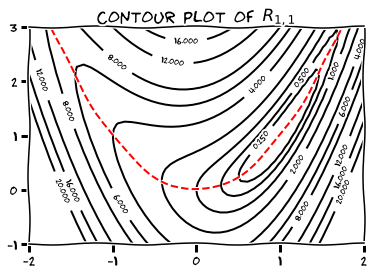
\includegraphics[width=0.5\linewidth]{rosenbrockContour} &
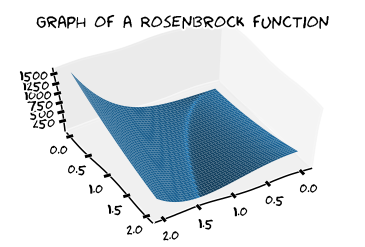
\includegraphics[width=0.5\linewidth]{rosenbrockGraph}
\end{tabular}
\caption{Details of the graph of $\mathcal{R}_{1,1}$}
\label{figure:Rosenbrock}
\end{figure}
It is also easy to verify that the image is the interval $[0,\infty)$.  Indeed, note first that $\mathcal{R}_{a,b}(x,y) \geq 0$ for all $(x,y) \in \field{R}^2$.  Zero is attained: $\mathcal{R}_{a,b} (a,a^2) = 0$.  Note also that $\mathcal{R}_{a,b}(0,y) = a^2 + by^2$ is a polynomial of degree 2, therefore unbounded.

Let's locate all local minima:
\begin{itemize}
	\item The gradient and Hessian are given respectively by
	\begin{equation*}
	\gradient{\mathcal{R}_{a,b}}(x,y) = \big[ 2(x-a) +4bx(x^2-y) , b(y-x^2) \big] \\
	\end{equation*}
	\begin{equation*}
	\Hess{\mathcal{R}_{a,b}}(x,y) = \begin{bmatrix}
	12bx^2-4by+2 & -4bx \\
	-4bx & 2b
	\end{bmatrix}
	\end{equation*}
	\item The search for critical points $\gradient{\mathcal{R}_{a,b}} = \boldsymbol{0}$ gives only the point $(a,a^2)$.
	\item $\frac{\partial^2 \mathcal{R}_{a,b}}{\partial x^2}(a,a^2) = 8ba^2+2 > 0$.
	\item The Hessian at that point has positive determinant:
	\begin{equation*}
	\det \Hess{\mathcal{R}_{a,b}}(a,a^2) = \det \begin{bmatrix}
	8ba^2+2 & -4ab \\
	-4ab & 2b
	\end{bmatrix} = 4b > 0
	\end{equation*}
\end{itemize}
There is only one local minimum at $(a,a^2)$, which happens also to be a global minimum.
\end{example}

The second step was the notion of \emph{global (or absolute) minima}: points $(x_0,y_0)$ that satisfy $f(x_0,y_0) \leq f(x,y)$ for any point $(x,y)$ in the domain of $f$.  We always started with the easier setting, in which we placed restrictions on the domain of our functions:

\begin{theorem}\label{theorem:MaxMinCompact}
A continuous real-valued function always attains its minimum value on a \emph{compact} set $K$. If the function is also differentiable in the \emph{interior} of $K$, to search for global minima we perform the following steps:
\begin{description}
	\item[Interior Candidates] List the critical points of $f$ located in the interior of $K$.
	\item[Boundary Candidates] List the points in the boundary of $K$ where $f$ may have minimum values.
	\item [Evaluation/Selection] Evaluate $f$ at all candidates and select the one(s) with the smallest value.
\end{description}
\end{theorem}

\begin{example}
A flat circular plate has the shape of the region 
\begin{equation*}
x^2+y^2 \leq 1.
\end{equation*} 
The plate, including the boundary, is heated so that the temperature at the point $(x,y)$ is given by $f(x,y) =100(x^2 +2 y^2 - x)$ in Celsius degrees.  Find the temperature at the coldest point of the plate.

We start by searching for critical points.  The equation $\gradient{f}(x,y) = 0$ gives $x=\tfrac{1}{2}$, $y=0$. The point $(\tfrac{1}{2}, 0)$ is clearly inside of the plate.  This is our first candidate.

The border of the plate can be parameterized by $\varphi(t) = (\cos t, \sin t)$ for $t \in [0,2\pi)$.  The search for minima in the boundary of the plate can then be coded as an optimization problem for the function $h(t) = (f \circ \varphi) (t) = 100(\cos^2 t + 2\sin^2 t - \cos t)$ on the interval $[0,2\pi)$.  Note that $h'(t) = 0$ for $t \in \{ 0, \tfrac{2}{3}\pi \}$ in $[0,2\pi)$.  We thus have two more candidates: 
\begin{equation*}
\varphi(0) = (1,0) \qquad \varphi(\tfrac{2}{3}\pi)= \big( -\tfrac{1}{2}, \tfrac{1}{2}\sqrt{3} \big)
\end{equation*}
Evaluation of the function at all candidates gives us the solution to this problem: 
\begin{equation*}
f( \tfrac{1}{2}, 0 ) = -25^\circ\mathrm{C}.
\end{equation*}
\end{example}

On a second setting, we remove the restriction of boundedness of the function.  In this case, global minima will only be guaranteed for very special functions.

\begin{example}\label{example:CoerciveFunctions}
Any polynomial $p_n(x) = a_n x^n + a_{n-1} x^{n-1} + \dotsb + a_0$ with even degree $n \geq 2$ and positive leading coefficient satisfies 
$\lim_{\abs{x}\to \infty} p_n(x) = +\infty$.  
To see this, we may write
\begin{equation*}
a_n x^n + a_{n-1} x^{n-1} + \dotsb + a_0 = a_n x^n \big( 1 + \tfrac{a_{n-1}}{a_n x} + \dotsb + \tfrac{a_0}{a_n x^n} \big)
\end{equation*}
The behavior of each of the factors as the absolute value of $x$ goes to infinity leads to our claim.
\begin{align*}
\lim_{\abs{x} \to \infty} a_n x^n &= +\infty, \\
\lim_{\abs{x} \to \infty} \big( 1 + \tfrac{a_{n-1}}{a_n x} + \dotsb + \tfrac{a_0}{a_n x^n} \big) &= 1.
\end{align*}
It is clear that a polynomial of this kind must attain a minimum somewhere in its domain. The critical points will lead to them.
\end{example}

\begin{example}
Find the global minima of the function $f(x)= \log (x^4-2x^2+2)$ in $\field{R}$.  

Note first that the domain of $f$ is the whole real line, since $x^4-2x^2+2 = (x^2-1)^2+1 \geq 1$ for all $x\ \in \field{R}$.  Note also that we can write $f(x) = (g \circ h)(x)$ with $g(x) = \log(x)$ and $h(x)=x^4-2x^2+1$.  Since $g$ is one-to-one and increasing, we can focus on $h$ to obtain the requested solution.  For instance, $\lim_{\abs{x}\to\infty}f(x) = +\infty$, since $\lim_{\abs{x}\to\infty} h(x) = +\infty$. This guarantees the existence of global minima.  To look for it, $h$ again points to the possible locations by solving for its critical points: $h'(x)=0$.  We have then that $f$ attains its minima at $x=\pm 1$.
\begin{figure}[ht!]
\begin{center}
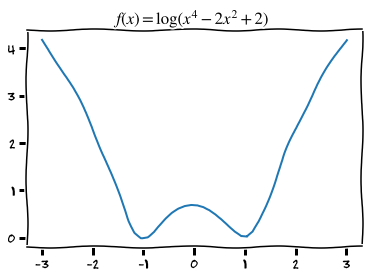
\includegraphics[width=0.5\linewidth]{coercivelog.png}
\end{center}
\caption{Global minima in unbounded domains}
\label{figure:coercivelog}
\end{figure}
\end{example}

We learned other useful characterizations for extrema, when the domain could be expressed as solutions of equations:

\begin{theorem}[Orthogonal Gradient]\label{theorem:OrthogonalGradient}
Suppose $f(x,y)$ is differentiable in a region whose interior contains a smooth curve $C\colon \boldsymbol{r}(t) = \big( x(t), y(t) \big)$.  If $P_0$ is a point on $C$ where $f$ has a local extremum relative to its values on $C$, then $\gradient{f}$ is orthogonal to $C$ at $P_0$.
\end{theorem}

This result leads to the \emph{Method of Lagrange Multipliers}

\begin{theorem}[Lagrange Multipliers on one constraint]\label{theorem:LM1C}
Suppose that $f(x,y)$ and $g(x,y)$ are differentiable and $\gradient{g} \neq 0$ when $g(x,y,z)=0$.  To find the local extrema of $f$ subject to the constraint $g(x,y)=0$ (if these exist), find the values of $x,y$ and $\lambda$ that simultaneously satisfy the equations
\begin{equation*}
\gradient{f} = \lambda \gradient{g}, \text{ and }g(x,y)=0
\end{equation*}
\end{theorem}

\begin{example}
Find the minimum value of the expression $3x+4y$ for values of $x$ and $y$ on the circle $x^2+y^2=1$.

We start by modeling this problem to adapt the technique of Lagrange multipliers:
\begin{align*}
f(x,y) &= \underbrace{3x+4y}_{\text{target}} & g(x,y)&=\underbrace{x^2+y^2-1}_{\text{constraint}}
\end{align*}
Look for the values of $x,y$ and $\lambda$ that satisfy the equations $\gradient{f} = \lambda\gradient{g}$, $g(x,y)=0$
\begin{align*}
3 &= 2\lambda x, & 4 &= 2\lambda y & 1 &= x^2+y^2 \\
\intertext{Equivalently, $\lambda \neq 0$ and $x,y$ satisfy}
x &= \frac{3}{2\lambda}, & y &= \frac{2}{\lambda}, &1 &= \frac{9}{4\lambda^2}+\frac{4}{\lambda^2}
\end{align*}
These equations lead to $\lambda = \pm \frac{5}{2}$, and there are only two possible candidates for minimum. Evaluation of $f$ on those gives that the minimum is at the point $\big(-\frac{3}{5}, -\frac{4}{5} \big)$.
\end{example}

This method can be extended to more than two dimensions, and more than one constraint.  For instance:
\begin{theorem}[Lagrange Multipliers on two constraints]\label{theorem:LM2C}
Suppose that $f(x,y,z)$, $g_1(x,y,z)$, $g_2(x,y,z)$ are differentiable with $\gradient{g_1}$ not parallel to $\gradient{g_2}$.  To find the local extrema of $f$ subject to the constraint $g_1(x,y,z)=g_2(x,y,z)=0$ (if these exist), find the values of $x,y, \lambda$ and $\mu$ that simultaneously satisfy the equations
\begin{align*}
\gradient{f} &= \lambda \gradient{g_1}+\mu\gradient{g_2}, &g_1(x,y,z)&=0, &g_2(x,y,z)&=0
\end{align*}
\end{theorem}

\begin{example}
The cylinder $x^2+y^2=1$ intersects the plane $x+y+z=1$ in an ellipse.  Find the points on the ellipse that lie closest to the origin.

We again model this as a Lagrange multipliers problem:
\begin{align*}
f(x,y,z) &= \overbrace{x^2+y^2+z^2}^{\text{target}}, \\ 
g_1(x,y,z)&= \underbrace{x^2+y^2-1}_{\text{constraint}}, & g_2(x,y,z) &= \underbrace{x+y+z-1}_{\text{constraint}}.
\end{align*}
The gradient equation $\gradient{f} = \lambda \gradient{g_1} + \mu \gradient{g_2}$ gives
\begin{align*}
2x &= 2\lambda x + \mu, &2y &= 2\lambda y+\mu, &2z &= \mu
\end{align*}
These equations are satisfied simultaneously only in two scenarios:
\begin{enumerate}
	\item $\lambda=1$ and $z=0$
	\item $\lambda \neq 1$ and $x=y=z/(1-\lambda)$
\end{enumerate} 
Resolving each case we find four candidates: 
\begin{equation*}
(1,0,0), \quad(0,1,0), \quad (\sqrt{2}/2, \sqrt{2}/2, 1- \sqrt{2}), \quad(-\sqrt{2}/2, -\sqrt{2}/2, 1+\sqrt{2}).
\end{equation*}  
The first two are our solution.
\end{example}

\section*{The Theory of Optimization}

The purpose of these notes is the development of a theory to deal with optimization in a more general setting.
\begin{itemize}
	\item We start in an Euclidean $d$--dimensional space with the usual topology based on the distance 
	\begin{equation*}
	\dist(\x,\y)=\norm{\x-\y} = \langle \x-\y, \x-\y \rangle^{1/2} = \sqrt{\sum_{k=1}^d (x_k-y_k)^2 }.
	\end{equation*}
	For instance, the \emph{open ball} of radius $r>0$ centered at a point $\xstar$ is the set $B_r(\xstar) = \{ \x \in \field{R}^d : \norm{\x-\xstar}< r \}.$
	\item Given a real-valued function $f\colon D \to \field{R}$ on a domain $D \subseteq \field{R}^d$, we define the concept of \emph{extrema} and \emph{extreme Values}:
	\begin{definition}\label{def:extrema}
	Given a real-valued function $f\colon D \to \field{R}$ on a domain $D \subseteq \mathbb{R}^d$, we say that a point $\xstar \in D$ is a:
	\begin{description}
		\item [global minimum] $f(\xstar) \leq f(\x)$ for all $\x \in D$.
		\item [global maximum] $f(\xstar) \geq f(\x)$ for all $\x \in D$.
		\item [strict global minimum] $f(\xstar) < f(\x)$ for all $\x \in D \setminus \{ \xstar \}$.
		\item [strict global maximum] $f(\xstar) > f(\x)$ for all $\x \in D \setminus \{ \xstar \}$.
		\item [local minimum] There exists $\delta>0$ so that  $f(\xstar) \leq f(\x)$ for all $\x \in B_\delta(\xstar)\cap D$.
		\item [local maximum] There exists $\delta>0$ so that  $f(\xstar) \geq f(\x)$ for all $\x \in B_\delta(\xstar)\cap D$.
		\item [strict local minimum] There exists $\delta>0$ so that  $f(\xstar) < f(\x)$ for all $\x \in B_\delta(\xstar)\cap D$, $\x \neq \xstar$.
		\item [strict local maximum] There exists $\delta>0$ so that  $f(\xstar) > f(\x)$ for all $\x \in B_\delta(\xstar)\cap D$, $\x \neq \xstar$.
	\end{description}
	\end{definition}	
\end{itemize}
In this setting, the objective of \emph{optimization} is the search for extrema in the following two scenarios:
\begin{description}
	\item [Unconstrained Optimization] if $D$ is an open set (usually the whole space $\field{R}^d$)
	\item [Constrained Optimization] if $D$ can be described as a set of \emph{constraints}: $\x \in D$ if there exist $m,n \in \field{N}$ and functions $g_k\colon \field{R}^d \to \field{R}$ ($1\leq k \leq m$), $h_j\colon \field{R}^d \to \field{R}$ ($1\leq j \leq n$) so that
	\begin{align*}
	g_k(\x) &\leq  0 \quad (1\leq k \leq m) \\
	h_j(\x) &= 0     \quad (1\leq j \leq n)
	\end{align*}
\end{description}
For each of these problems, we follow a similar program:
\begin{description}
	\item[Existence of extrema] Establish results that guarantee the existence of extrema depending on the properties of $D$ and $f$. 
	\item[Characterization of extrema] Establish results that describe conditions for points $\x \in D$ to be extrema of $f$.  
	\item[Tracking extrema] Design robust numerical algorithms that find the extrema for scientific computing purposes.
\end{description}
The development of existence and characterization results for unconstrained optimization will be covered in chapter \ref{chapter:UnconstrainedExistenceCharacterization}.  The design of algorithms to track extrema in the unconstrained setting will be covered in chapter \ref{chapter:UnconstrainedNumerical}.  Chapter \ref{chapter:ConstrainedExistenceCharacterization} is devoted to existence and characterization results for constrained optimization, and Chapter \ref{chapter:ConstrainedNumerical} for the design of algorithms in that setting.










%!TEX root = main.tex

\section*{Exercises}
\begin{problem}[Advanced]
State and prove similar statements as in Definition \ref{def:localminimum}, Theorems \ref{theorem:localminimum}, \ref{theorem:2DTforLEV} and \ref{theorem:MaxMinCompact}, but for \emph{local} and \emph{global maxima}.
\end{problem}

\begin{problem}[Basic]
Find and sketch the domain of the following functions.
\begin{enumerate}
	\item $f(x,y) = \sqrt{y-x-2}$
	\item $f(x,y) = \log \big( x^2+y^2-4 \big)$
	\item $f(x,y) = \frac{(x-1)(y+2)}{(y-x)(y-x^3)}$
	\item $f(x,y) = \log (xy+x-y-1)$
\end{enumerate}
\end{problem}

\begin{problem}[Basic]
Find and sketch the level lines $f(x,y)=c$ on the same set of coordinate axes for the given values of $c$.
\begin{enumerate}
	\item $f(x,y) = x+y-1$, $c \in \{ -3, -2, -1, 0, 1, 2, 3\}$.
	\item $f(x,y) = x^2+y^2$, $c \in \{ 0, 1, 4, 9, 16, 25 \}$.
	\item $f(x,y) = xy$, $c \in \{ -9, -4, -1, 0, 1, 4, 9 \}$
\end{enumerate}
\end{problem}

\begin{problem}[CAS]\label{problem:countours}
Use a Computer Algebra System of your choice to produce contour plots of the given functions on the given domains.
\begin{enumerate}
	\item $f(x,y) = (\cos x)(\cos y) e^{-\sqrt{x^2+y^2}/4}$ on $[-2\pi, 2\pi]\times [-2\pi, 2\pi]$.
	\item $g(x,y) = \dfrac{xy(x^2-y^2)}{x^2+y^2}$ on $[-1,1] \times [-1,1]$
	\item $h(x,y) = y^2 - y^4 -x^2$ on $[-1,1]\times[-1,1]$
	\item $k(x,y) = e^{-y}\cos x$ on $[-2\pi, 2\pi]\times[-2,0]$
\end{enumerate}
\begin{figure}[ht!]
\begin{tabular}{cc}
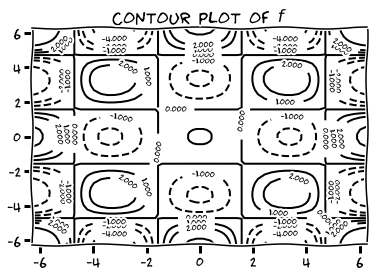
\includegraphics[width=0.5\linewidth]{images/contourf.png} &
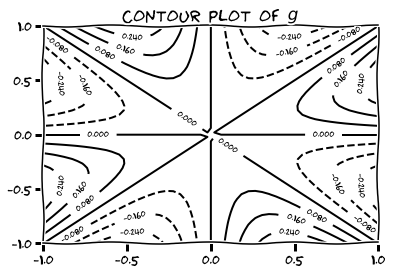
\includegraphics[width=0.5\linewidth]{images/contourg.png} \\
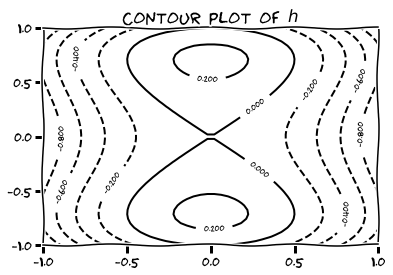
\includegraphics[width=0.5\linewidth]{images/contourh.png} &
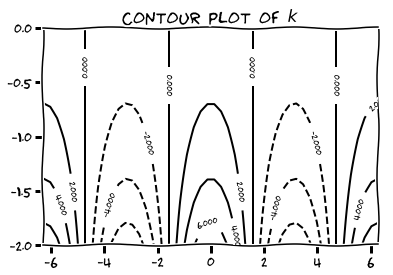
\includegraphics[width=0.5\linewidth]{images/contourk.png} 
\end{tabular}
\caption{Contour plots for problem \ref{problem:countours}}
\end{figure}
\end{problem}

\begin{problem}[Basic]
Sketch the curve $f(x,y)=c$ together with $\gradient{f}$ and the tangent line at the given point.  Write an equation for the tangent line.
\begin{enumerate}
	\item $f(x,y)=x^2+y^2$, $c=4$, $(\sqrt{2}, \sqrt{2})$.
	\item $f(x,y)=x^2-y$, $c=1$, $(\sqrt{2}, 1)$.
	\item $f(x,y)=xy$, $c=-1$, $(2, -2)$.
	\item $f(x,y)=x^2-xy+y^2$, $c=7$, $(-1,2)$.
\end{enumerate}
\end{problem}

\begin{problem}[Basic]
For the function
\begin{equation*}
f(x,y) = \frac{x-y}{x+y},
\end{equation*}
at the point $P_0 = (-1/2, 3/2)$, find the directions $\boldsymbol{v}$ and the directional derivatives $D_{\boldsymbol{v}}f(P_0)$ for which
\begin{enumerate}
	\item $D_{\boldsymbol{v}}f(P_0)$ is largest.
	\item $D_{\boldsymbol{v}}f(P_0)$ is smallest.
	\item $D_{\boldsymbol{v}}f(P_0) = 0$.
	\item $D_{\boldsymbol{v}}f(P_0) = 1$.
	\item $D_{\boldsymbol{v}}f(P_0) = -2$.
\end{enumerate}
\end{problem}

\begin{problem}[Intermediate]
The derivative of $f(x,y)$ at $(1,2)$ in the direction $\frac{\sqrt{2}}{2}[1,1]$ is $2\sqrt{2}$ and in the direction $[0,-1]$ is $-3$.  What is the derivative of $f$ in the direction $\frac{\sqrt{5}}{5}[-1,-2]$?
\end{problem}

\begin{problem}[Intermediate]
Find the absolute maxima and minima of the function $f(x,y) = (4x-x^2)\cos y$ on the rectangular plate $1\leq x \leq 3, -\frac{\pi}{4} \leq y \leq \frac{\pi}{4}$.
\end{problem}

\begin{problem}[Basic]
Find two numbers $a \leq b$ such that 
\begin{equation*}
\int_a^b (24-2x-x^2)^{1/3}\, dx
\end{equation*}
has its largest value.
\end{problem}

\begin{problem}[Basic] % example 2, p.858 in Thomas' Calculus
Find the points of the hyperbolic cylinder $x^2-z^2-1=0$ in $\field{R}^3$ that are closest to the origin.
\end{problem}

\begin{problem}[Intermediate]
Find the extreme values of the function $f(x,y,z)=xy+z^2$ on the circle in which the plane $y-x=0$ intersects the sphere $x^2+y^2+z^2=4$.
\end{problem}

\begin{problem}[CAS]
Write a routine (in your favorite CAS) that uses \emph{symbolic computation} to find the minimum of a real-valued function $f \colon \field{R} \to \field{R}$ over 
\begin{enumerate}
	\item a closed interval $[a,b]$
	\item An interval of the form $[a,\infty)$, or $(-\infty, b]$
\end{enumerate}
The routine should accept as input:
\begin{itemize}
	\item the expression of the function $f$,
	\item the endpoints $a,b$.
\end{itemize}
\end{problem}

%%%%% chapter 2
\chapter[Unconstrained Optimization]{Existence and Characterization of Extrema for Unconstrained Optimization}
\label{chapter:UnconstrainedExistenceCharacterization}
%!TEX root = main.tex

\chapter[Unconstrained Optimization]{Existence and Characterization of Extrema for Unconstrained Optimization}\label{chapter:UnconstrainedExistenceCharacterization}

In this chapter we will study different properties of functions and domains that guarantee existence of extrema for unconstrained optimization. Once we have them, we explore characterization of those points.  We start with a reminder of the definition of continuous and differentiable functions, and then we proceed to introduce other functions with advantageous properties for optimization purposes.

\section{Anatomy of a function}

\subsection{Continuity and Differentiability}

\begin{definition}\label{def:continuous}\index{Function!continuous}
We say that a function $\boldsymbol{f} \colon \field{R}^{d_1} \to \field{R}^{d_2}$ is continuous at a point $\xstar \in \field{R}^{d_1}$ if for all $\varepsilon > 0$ there exists $\delta > 0$ so that for all $\x \in \field{R}^{d_1}$ satisfying $\norm{\x-\xstar}_{d_1}<\delta$, it is $\norm{ f(\x) - f(\xstar) }_{d_2} < \varepsilon$.  
\end{definition}

\begin{example}
Let $f\colon \field{R}^2 \to \field{R}$ be given by
\begin{equation*}
f(x,y) = \begin{cases}
\frac{2xy}{x^2+y^2}, &(x,y) \neq (0,0) \\
0, &(x,y)=(0,0)
\end{cases}
\end{equation*}
This function is trivially continuous at any point $(x,y)\neq(0,0)$.  However, it fails to be continuous at the origin.  Notice how we obtain different values as we approach $(0,0)$ through different generic lines $y=mx$ with $m \in \field{R}$:
\begin{equation*}
\lim_{x\to 0} f(x,mx) = \lim_{x \to 0} \frac{2mx^2}{(1+m^2)x^2} = \frac{2m}{1+m^2}.
\end{equation*}
\end{example}

\begin{definition}\label{def:linearMap}\index{Linear map}\index{Linear transformation|see {Linear map}}\index{kernel}\index{image}
A function $\boldsymbol{T} \colon \field{R}^{d_1} \to \field{R}^{d_2}$ is said to be a \emph{linear map} (or a \emph{linear transformation}) if it satisfies 
\begin{equation*}
\boldsymbol{T}(\x+\lambda\y) = \boldsymbol{T}(\x) + \lambda \boldsymbol{T}(\y) \text{ for all }\x, \y \in \field{R}^{d_1}, \lambda \in \field{R}.
\end{equation*}  
The \emph{kernel} and \emph{image} of a linear map are respectively given by
\begin{align*}
\ker T & = \{ \x \in \field{R}^{d_1} : T(\x) = \boldsymbol{0} \}, \\
\operatorname{im} T &= \{ \y \in \field{R}^{d_2} : \text{ there exists }\x \in \field{R}^{d_1} \text{ so that }\y = T(\x) \}.
\end{align*}
\end{definition}

\begin{remark}
For each real-valued linear map $T \colon \field{R}^d \to \field{R}$ there exists $\boldsymbol{a} \in \field{R}^d$ so that $T(\x) = \langle \boldsymbol{a} , \x \rangle$ for all $\x \in \field{R}^d$.

The kernel of a linear map in this case has a very simple expression:
\begin{equation*}
\ker T = \ker \langle \boldsymbol{a}, \cdot \rangle = \{ (x_1, x_2, \dotsc, x_d) \in \field{R}^d : a_1 x_1 + a_2 x_2 + \dotsb + a_d x_d = 0 \}
\end{equation*}

The graph of a real-valued linear function can be identified with a hyperplane in $\field{R}^{d+1}$ :
\begin{align*}
\operatorname{Graph} T &= \{ (\x,y) \in \field{R}^{d+1} : y = T(\x) \} \\
&= \{ (x_1, x_2, \dotsc, x_d, y) \in \field{R}^{d+1} : a_1x_1 + a_2 x_2 + \dotsb + a_dx_d = y \} \\
& = \ker \langle [a_1, a_2, \dotsc, a_d, -1], \cdot \rangle
\end{align*}
\end{remark}

\begin{remark}
For each linear map $\boldsymbol{T} \colon \field{R}^{d_1} \to \field{R}^{d_2}$ there exists a matrix $\boldsymbol{A}$ of size $d_1 \times d_2$ so that $\transpose{\boldsymbol{T}(\x)} = \boldsymbol{A} \cdot \transpose{\x}$.
\begin{equation*}
\begin{cases} 
y_1 &= a_{11} x_1 + \dotsb + a_{1d_1} x_{d_1} \\ 
y_2 &= a_{21} x_1 + \dotsb + a_{2d_1} x_{d_1} \\
    &\vdots \\
y_{d_2} &= a_{d_2 1} x_1 + \dotsb + a_{d_1 d_2} x_{d_1}
\end{cases}
\end{equation*}
\end{remark}

\begin{definition}\label{def:differentiable}\index{Function!differentiable}
A function $\boldsymbol{f} \colon \field{R}^{d_1} \to \field{R}^{d_2}$ is said to be \emph{differentiable} at $\xstar$ if there exists a \emph{linear map} $\boldsymbol{J} \colon \field{R}^{d_1} \to \field{R}^{d_2}$ so that 
\begin{equation*}
\lim_{\boldsymbol{h} \to \boldsymbol{0}} \frac{\norm{\boldsymbol{f}(\xstar+\boldsymbol{h})-\boldsymbol{f}(\xstar)-\boldsymbol{J}(\boldsymbol{h})}_{d_2}}{\norm{\boldsymbol{h}}_{d_1}} = 0
\end{equation*}
\end{definition}

 
\begin{example}\label{example:derivatives}
Consider a real-valued function $f\colon \field{R} \to \field{R}$ of a real variable. To prove differentiability at a point $x^\star$, we need a linear map: $J(h)=ah$ for some $a\in \field{R}$. Notice how in that case, 
\begin{equation*}
\frac{\abs{f(x^\star+h)-f(x^\star)-J(h)}}{\abs{h}} = \left\lvert \frac{f(x^\star+h)-f(x^\star)}{h} - a \right\lvert;
\end{equation*}
therefore, we could pick $a = \lim_{h\to 0} h^{-1}\big( f(x^\star+h) - f(x^\star) \big)$---this is the definition of derivative we learned in Calculus: $a=f'(x^\star)$.
\end{example}

\begin{remark}\index{Matrix!Jacobian}\index{Jacobian}\index{Derivative!partial}\index{Derivative!directional}
If a function $\boldsymbol{f} \colon \field{R}^{d_1} \to \field{R}^{d_2}$ is differentiable at $\xstar$, then all of the partial derivatives exist at $\xstar$, in which case the linear map $\boldsymbol{J}$ is given by the \emph{Jacobian matrix}
\begin{equation*}
\boldsymbol{J}(\x) = \begin{bmatrix} 
\frac{\partial f_1}{\partial x_1} & \frac{\partial f_1}{\partial x_2} & \dotsb & \frac{\partial f_1}{\partial x_{d_1}} \\
\frac{\partial f_2}{\partial x_1} & \frac{\partial f_2}{\partial x_2} & \dotsb & \frac{\partial f_2}{\partial x_{d_1}} \\
\vdots & \vdots & \ddots & \vdots \\
\frac{\partial f_{d_2}}{\partial x_1} & \frac{\partial f_{d_2}}{\partial x_2} & \dotsb & \frac{\partial f_{d_2}}{\partial x_{d_1}} \\
\end{bmatrix} \cdot \begin{bmatrix}
x_1 \\ x_2 \\ \vdots \\ x_{d_1} 
\end{bmatrix}
\end{equation*}
The converse is not true in general: the existence of partial derivatives (or even all of the directional derivatives) is not guarantee that a function is differentiable at a point.  For instance, the function $f \colon \field{R}^2 \to \field{R}$ given by
\begin{equation*}
f(x,y) = \begin{cases} 
y^3/(x^2+y^2) &\text{if }(x,y) \neq (0,0) \\
0 &\text{if }(x,y) = (0,0) \end{cases}
\end{equation*}
is not differentiable at $(0,0)$, although all partial derivatives and all directional derivatives exist at that point.
\end{remark}


\separator 

A \emph{friendly} version of the differentiability of real-valued functions comes with the next result (see, e.g.~\cite[p.818]{finney2001thomas})
\begin{theorem}\label{theorem:partialgivesDerivative}
If the partial derivatives $\frac{\partial f}{\partial x_1}, \dotsc, \frac{\partial f}{\partial x_d}$ of a real-valued function $f \colon \field{R}^d \to \field{R}$ are continuous on an open region $G \subseteq \field{R}^d$, then $f$ is differentiable at every point of $G$.
\end{theorem}

\begin{example}\label{example:gradient}
Let $f\colon \field{R}^d \to \field{R}$.  To prove that $f$ is differentiable at a point $\xstar \in \field{R}^d$ we need a linear map $J(h) = \langle \boldsymbol{a}, h \rangle$ for some $\boldsymbol{a} \in \field{R}^d$.  Under the conditions of Theorem \ref{theorem:partialgivesDerivative} we may use
\begin{equation*}
\boldsymbol{a} = \gradient{f}(\xstar)= \bigg[ \frac{\partial f (\xstar)}{\partial x_1}, \dotsc, \frac{\partial f (\xstar)}{\partial x_d} \bigg],
\end{equation*}
if we are able to prove that all partial derivatives are continuous in an open set containing $\xstar$.
\end{example}

\separator 

It is a simple task to prove that all differentiable functions are continuous.  Is it true that all continuous functions are differentiable?

\begin{example}[Weierstrass Function]\label{example:WeierstrassFunction}\index{Function!Weierstrass}
For any positive real numbers $a, b$ satisfying $0<a<1<b$ and $ab \geq 1$, consider the Weierstrass function $\mathcal{W}_{a,b} \colon \field{R} \to \field{R}$ given by 
\begin{equation*}
\mathcal{W}_{a,b}(x) = \sum_{n=0}^\infty a^n \cos(b^n \pi x)
\end{equation*}
This function is continuous everywhere, yet \emph{nowehere} differentiable! (see Figure~\ref{figure:WeierstrassFunction}). For a proof, see e.g.~\cite{hardy1916weierstrass}
\begin{figure}[ht!]
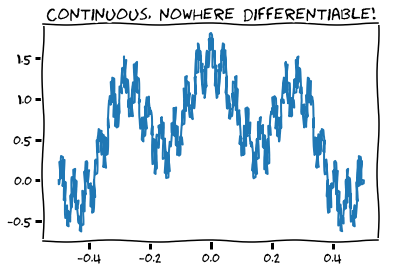
\includegraphics[width=0.6\linewidth]{images/weierstrass.png}
\caption{Detail of the graph of $\mathcal{W}_{0.5, 7}$}
\label{figure:WeierstrassFunction}
\end{figure}
\end{example}

\separator

A few more useful results about higher order derivatives follow:

\begin{theorem}[Clairaut]\label{theorem:MixedDerivatives}\index{Theorem!Clairaut}
If $f\colon \field{R}^d \to \field{R}$ and its partial derivatives of orders 1 and 2, $\frac{\partial f}{\partial x_k}$, $\frac{\partial^2 f}{\partial x_k \partial x_j}$, ($1\leq k,j \leq d$) are defined throughout an open region containing the point $\xstar$, and are all continuous at $\xstar$, then 
\begin{equation*}
\frac{\partial^2 f(\xstar)}{\partial x_k \partial x_j} = \frac{\partial^2 f(\xstar)}{\partial x_j \partial x_k}, \quad (1\leq k,j \leq d). 
\end{equation*}
\end{theorem}

\begin{definition}[Hessian]\label{def:Hessian}\index{Hessian}
Given a twice-differentiable function $f\colon \field{R}^d \to \field{R}$, we define the \emph{Hessian} of $f$ at $\x$ to be the following matrix of second partial derivatives:
\begin{equation*}
\Hess{f}(\x) = \begin{bmatrix}
\frac{\strut\partial^2 f (\x)}{\strut\partial x_1^2} & \frac{\strut\partial^2 f (\x)}{\strut\partial x_1 \partial x_2} &\dotsb &\frac{\strut\partial^2 f (\x)}{\strut\partial x_1 \partial x_d} \\
&&&\\
\frac{\strut\partial^2 f (\x)}{\strut\partial x_2 \partial x_1} & \frac{\strut\partial^2 f (\x)}{\strut\partial x_2^2} &\dotsb &\frac{\strut\partial^2 f (\x)}{\strut\partial x_2 \partial x_d} \\
&&& \\
\vdots & \vdots &\ddots &\vdots \\
&&& \\
\frac{\strut\partial^2 f (\x)}{\strut\partial x_d \partial x_1} & \frac{\strut\partial^2 f (\x)}{\strut\partial x_d \partial x_2} &\dotsb &\frac{\strut\partial^2 f (\x)}{\strut\partial x_d^2}
\end{bmatrix}
\end{equation*}
\end{definition}

\separator

Functions that satisfy the conditions of Theorem \ref{theorem:MixedDerivatives} have symmetric Hessians.  We shall need some properties in regard to symmetric matrices.

\begin{definition}\index{Matrix!Symmetric}\index{Quadratic Form}\index{Matrix!Symmetric!Positive Definite}\index{Matrix!Symmetric!Positive Semidefinite}\index{Matrix!Symmetric!Negative Definite}\index{Matrix!Symmetric!Negative Semidefinite}\index{Matrix!Symmetric!Indefinite}
Given a symmetric matrix $\boldsymbol{A}$, we define its associated \emph{quadratic form} as the function $\quadratic{A}\colon \field{R}^d \to \field{R}$ given by
\begin{equation*}
\quadratic{A}(\x) = \x \boldsymbol{A} \transpose{\x} = \begin{bmatrix} x_1 \dotsb x_d \end{bmatrix} \begin{bmatrix} a_{11} &\dotsb &a_{1d} \\ \vdots & \ddots & \vdots \\ a_{1d} &\dotsb &a_{dd} \end{bmatrix} \begin{bmatrix} x_1 \\ \vdots \\ x_d \end{bmatrix}
\end{equation*}
We say that a symmetric matrix is:
\begin{description}
\item[positive definite] if $\quadratic{A}(\x) > 0$ for all $\x \in \field{R}^d \setminus \{ \boldsymbol{0} \}$.
\item[positive semidefinite] if $\quadratic{A}(\x)\geq 0$ for all $\x \in \field{R}^d$.
\item[negative definite] if $\quadratic{A}(\x) < 0$ for all $\x \in \field{R}^d \setminus \{ \boldsymbol{0} \}$.
\item[negative semidefinite] if $\quadratic{A}(\x) \leq 0$ for all $\x \in \field{R}^d$.
\item[indefinite] if there exist $\x, \y \in \field{R}^d$ so that $\quadratic{A}(\x) \quadratic{A}(\y) < 0$. 
\end{description}
\end{definition}

\begin{example}\label{example:quadraticFromMatrix}
Let $\boldsymbol{A}$ be the $3\times 3$--symmetric matrix
\begin{equation*}
\boldsymbol{A} = \begin{bmatrix} 2 & -1 & 2 \\ -1 & 3 & 0 \\ 2 & 0 & 5 \end{bmatrix}
\end{equation*}
The associated quadratic form is given by
\begin{align*}
\quadratic{A}(x,y,z) &= \begin{bmatrix} x & y & z \end{bmatrix} \begin{bmatrix} 2 & -1 & 2 \\ -1 & 3 & 0 \\ 2 & 0 & 5 \end{bmatrix} \begin{bmatrix} x \\ y \\ z \end{bmatrix} \\
&= \begin{bmatrix} x & y & z \end{bmatrix} \begin{bmatrix} 2x -y +2z \\ -x+3y \\ 2x+5z \end{bmatrix} \\
&= x(2x-y+2z) + y(-x+3y) + z(2x+5z) \\
&= 2x^2 +3y^2 + 5z^2 -2xy +4xz
\end{align*}
\end{example}

\separator 

To easily classify symmetric matrices, we usually employ any of the following two criteria:

\begin{theorem}[Principal Minor Criteria]\label{theorem:PrincipalMinors}\index{Theorem!Principal Minor Criteria}
Given a general square matrix $\boldsymbol{A}$, we define for each $1\leq \ell \leq d$, $\Delta_\ell$ (the $\ell$th \emph{principal minor} of $\boldsymbol{A}$) to be the determinant of the upper left-hand corner $\ell \times \ell$--submatrix of $\boldsymbol{A}$.  
\begin{center}
\begin{tikzpicture}
\draw (0,0) node{%
$\begin{bmatrix}
a_{11} & a_{12} & a_{13} & \dotsb & a_{1n} \\
a_{21} & a_{22} & a_{23} & \dotsb & a_{2n} \\
a_{31} & a_{32} & a_{33} & \dotsb & a_{3n} \\
\vdots & \vdots & \vdots & \ddots & \vdots \\
a_{n1} & a_{n2} & a_{n3} & \dotsb & a_{nn} 
\end{bmatrix}$};
\draw[dashed] (-2, 0.73) -- (-1.35, 0.73) -- (-1.35, 1.2) node[above]{$\Delta_1$};
\draw[dashed] (-2, 0.27) -- (-0.5, 0.27) -- (-0.5, 1.2) node[above]{$\Delta_2$};
\draw[dashed] (-2, -0.15) -- (0.4, -0.15) -- (0.4, 1.2) node[above]{$\Delta_3$};
\end{tikzpicture}
\end{center}
A symmetric matrix $\boldsymbol{A}$ is:
\begin{itemize}
\item Positive definite if and only if $\Delta_\ell > 0$ for all $1\leq \ell \leq d$.
\item Negative definite if and only if $(-1)^\ell \Delta_\ell>0$ for all $1\leq \ell \leq d$.
\end{itemize}
\end{theorem}

\begin{example}
The matrix $\boldsymbol{A}$ in Example \ref{example:quadraticFromMatrix} is positive definite:
\begin{align*}
\Delta_1 &= 2 > 0 \\
\Delta_2 &= \det \begin{bmatrix} 2 & -1 \\ -1 & 3 \end{bmatrix} = 5 > 0 \\
\Delta_3 &= \det \boldsymbol{A} = 2 \det \begin{bmatrix} -1 & 3 \\ 2 & 0 \end{bmatrix} + 5 \det \begin{bmatrix} 2 & -1 \\ -1 & 3 \end{bmatrix} = 13 >0
\end{align*}
\end{example}

\begin{theorem}[Eigenvalue Criteria]\label{theorem:eigenvalues}\index{Characteristic Polynomial}\index{Eigenvalue}\index{Theorem!Eigenvalue Criteria}
Given a general square $d \times d$ matrix $\boldsymbol{A}$, consider the function $p_{\boldsymbol{A}} \colon \field{C} \to \field{C}$ given by $p_{\boldsymbol{A}}(\lambda) = \det\big(\boldsymbol{A} - \lambda \boldsymbol{I}_d \big)$.  This is a polynomial of (at most) degree $d$ in $\lambda$.  We call it the \emph{characteristic polynomial} of $\boldsymbol{A}$.  The roots (in $\field{C}$) of the characteristic polynomial are called the \emph{eigenvalues} of $\boldsymbol{A}$.  Symmetric matrices enjoy the following properties:
\begin{enumerate}
	\item The eigenvalues of a symmetric matrix are all real.
	\item If $\lambda \in \field{R}$ is a root  of multiplicity $n$ of the characteristic polynomial of a (non-trivial) symmetric matrix, then there exist $n$ linearly independent vectors $\{ \x_1, \x_2, \dotsc, \x_n \}$ satisfying $\boldsymbol{A} \x_k = \lambda \x_k$ ($1\leq k \leq n$).
	\item If $\lambda_1 \neq \lambda_2$ are different roots of the characteristic polynomial of a symmetric matrix, and $\x_1, \x_2 \in \field{R}^d$ satisfy $\boldsymbol{A} \x_k = \lambda_k \x_k$ ($k=1,2$), then $\langle \x_1, \x_2 \rangle = 0$.
	\item A symmetric matrix is positive definite (resp.~negative definite) if and only if all its eigenvalues are positive (resp.~negative).
	\item A symmetric matrix is positive semidefinite (resp.~negative semidefinite) if and only if all its eigenvalues are non-negative (resp.~non-positive)
	\item A symmetric matrix is indefinite if there exist two eigenvalues $\lambda_1 \neq \lambda_2$ with different sign.
\end{enumerate}
\end{theorem}

\begin{example}
Let's compute the eigenvalues of matrix $\boldsymbol{A}$ in Example \ref{example:quadraticFromMatrix}:
\begin{align*}
\det (\boldsymbol{A} - \lambda \boldsymbol{I}) &= \det \begin{bmatrix}
2-\lambda & -1 & 2 \\ -1 & 3-\lambda & 0 \\ 2 & 0 & 5-\lambda \end{bmatrix} \\
& = 2 \det\begin{bmatrix} -1 & 2 \\ 3-\lambda & 0 \end{bmatrix} + 5 \det \begin{bmatrix} 2-\lambda & -1 \\ -1 & 3-\lambda \end{bmatrix} \\
&= -4(3-\lambda) + 5 \big( (2-\lambda)(3-\lambda) -1 \big) \\
& = -\lambda^3 + 10\lambda^2 - 30\lambda + 25 \\
& = (\lambda - 5) (-\lambda^2 + 5\lambda - 5).
\end{align*}
Notice that this polynomial has three real roots: $\lambda_1 = 5$, $\lambda_2 = \tfrac{5+\sqrt{5}}{2} \approx 3.618$, and $\lambda_3 = \tfrac{5-\sqrt{5}}{2} \approx 1.381966$, all of them positive (as we expected).
\end{example}

\subsection{Coercive Functions}
Other set of functions that play an important role in optimization are the kind of functions we explored in Example \ref{example:CoerciveFunctions}.

\begin{definition}[Coercive functions]\label{def:coerciveFunctions}\index{Function!coercive}
A continuous real-valued function $f$ is said to be \emph{coercive} if for all $M>0$ there exists $R=R(M)>0$ so that $f(\x)\geq M$ if $\norm{\x}\geq R$.
\end{definition}

\begin{remark}
This is equivalent to the limit condition  
\begin{equation*}
\lim_{\norm{\x}\to \infty} f(\x) = +\infty.
\end{equation*}
\end{remark}

\begin{example}\label{example:CoerciveFunctionsGeneral}
We saw in Example \ref{example:CoerciveFunctions} how even-degree polynomials with positive leading coefficients are coercive, and how this helped guarantee the existence of a minimum.

We must be careful assessing coerciveness of polynomials in higher dimension. Consider for example $p_2(x,y) = x^2 - 2xy + y^2$.  Note how $p_2(x,x)=0$ for any $x \in \field{R}$, which proves $p_2$ is not coercive.

To see that the polynomial $p_4(x, y) = x^4 + y^4 - 4xy$ is coercive, we start by factoring the leading terms:
\begin{equation*}
x^4 + y^4 - 4xy = \big( x^4 + y^4 \big) \bigg( 1 - \frac{4xy}{x^4 + y^4} \bigg)
\end{equation*}
Assume $r>1$ is large, and that $x^2+y^2 = r^2$.  We have then
\begin{align*}
x^4 + y^4 &\geq \frac{r^4}{2} \qquad\text{(Why?)} \\
% Do x=rcos(theta) y=rsin(theta) and note x^4+y^4=r^4(cos^(theta)+sin^4(theta))
 \abs{x y} &\leq \frac{r^2}{2} \qquad\text{(Why?)}
% Same x,y, to see that xy = r^2cos(theta)sin(theta) = r^2 sin(2theta)/2
\end{align*}
therefore, 
\begin{align*}
\frac{4xy}{x^4 + y^4} &\leq \frac{4}{r^2} \\
1 - \frac{4xy}{x^4 + y^4} &\geq 1 - \frac{4}{r^2} \\
\big( x^4 + y^4 \big) \bigg( 1 - \frac{4 x y}{x^4 + y^4} \bigg) &\geq \frac{r^2(r^2-4)}{2}
\end{align*} 
We can then conclude that given $M>0$, if $x^2+y^2 \geq  2+\sqrt{4+2M}$, then $p_4(x,y) \geq M$.  This proves $p_4$ is coercive.
\end{example}

\subsection{Convex Functions}

There is one more kind of functions we should explore.

\begin{definition}[Convex Sets]\label{def:convexSets}\index{Convex!set}
A subset $C \subseteq \field{R}^d$ is said to be \emph{convex} if for every $\x, \y \in C$, and every $\lambda \in [0,1]$, the point $\lambda \y + (1-\lambda) \x$ is also in $C$.
\end{definition}

\separator 

The following result is an interesting characterization of convex sets that allows us to actually construct any convex set from a family of points.
\begin{theorem}
Let $C\subseteq \field{R}^d$ be a convex set and let $\{ \x_1, \x_2, \dotsc, \x_n \} \subset C$ be a family of points in $C$.  The convex combinations $\lambda_1 \x_1 + \lambda_2 \x_2 + \dotsb + \lambda_n \x_n$ are also in $C$, provided $\lambda_k\geq 0$ for all $1\leq k \leq n$ and $\lambda_1 + \lambda_2 + \dotsb + \lambda_n = 1$.
\end{theorem}

\begin{figure}[ht!]
\begin{tabular}{cc}
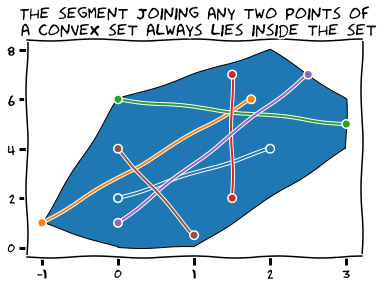
\includegraphics[width=0.48\linewidth]{images/convexSet1.png} &
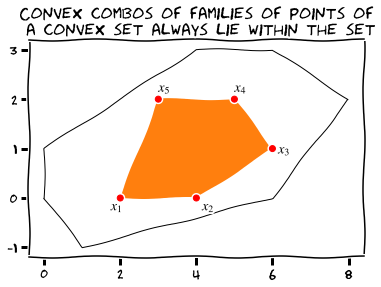
\includegraphics[width=0.48\linewidth]{images/convexSet2.png}
\end{tabular}
\caption{Convex sets.}
\label{figure:convexSet}
\end{figure}

\begin{definition}[Convex Functions]\label{def:ConvexFunctions}\index{Function!convex}\index{Convex!function}\index{Function!strictly convex}
Given a convex set $C \subseteq \field{R}^d$, we say that a real-valued function $f \colon C \to \field{R}$ is \emph{convex} if 
\begin{equation*}
f\big(\lambda \y + (1-\lambda)\x \big) \leq \lambda f(\y) + (1-\lambda) f(\x)
\end{equation*}
If instead we have $f\big(\lambda \x + (1-\lambda)f(\y)\big) < \lambda f(\x) + (1-\lambda) f(\y)$ for $0<\lambda<1$, we say that the function is \emph{strictly convex}.  A function $f$ is said to be \emph{concave} (resp.~\emph{strictly concave}) if $-f$ is convex (resp.~strictly convex).
\end{definition}

\begin{remark}\index{Epigraph}
There is an alternative definition of convex functions using the concept of \emph{epigraph} of a function.  Given a convex function $f\colon C \to \field{R}$ on a convex set $C$, the epigraph of $f$ is a set $\epi(f) \subset \field{R}^{d+1}$ defined by
\begin{equation*}
\epi(f) = \{ (\x,y) \in \field{R}^{d+1} : \x \in C, y \in \field{R}, f(\x) \leq y \}.
\end{equation*}
The function $f$ is convex if and only if its epigraph is a convex set.
\end{remark}

\separator

Convex functions have many pleasant properties:
\begin{theorem}\label{theorem:ConvexIsContinuous}
Convex functions are continuous.
\end{theorem}

\begin{theorem}
Let $f\colon C \to \field{R}$ be a real-valued convex function defined on a convex set $C \subseteq \field{R}^d$.  If $\lambda_1, \dotsc, \lambda_n$ are nonnegative numbers satisfying $\lambda_1 + \dotsb + \lambda_n = 1$ and $\x_1, \dotsc, x_n$ are $n$ different points in $C$, then
\begin{equation*}
f\big( \lambda_1 \x_1 + \dotsb + \lambda_n x_n \big) \leq \lambda_1 f(\x_1) + \dotsb + \lambda_n f(\x_n).
\end{equation*}
\end{theorem}

\begin{theorem}\label{theorem:convexAboveTangentHyperplane}
If $f\colon C \to \field{R}$ is a function on a convex set $C \subseteq \field{R}^d$ with continuous first partial derivatives on $C$, then
\begin{enumerate}
	\item $f$ is convex if and only if for all $\x, \y \in C$,
	\begin{equation*}
	f(\x) + \langle \gradient{f}(\x), \y - \x \rangle \leq f(\y).
	\end{equation*}
	\item $f$ is strictly convex if for all $\x \neq \y \in C$,
	\begin{equation*}
	f(\x) + \langle \gradient{f}(\x), \y - \x \rangle < f(\y).
	\end{equation*}
\end{enumerate}
\end{theorem}

\begin{remark}
Theorem \ref{theorem:convexAboveTangentHyperplane} implies that the graph of any (strictly) convex function always lies over the tangent hyperplane at any point of the graph.
\begin{figure}[ht!]
\begin{tabular}{cc}
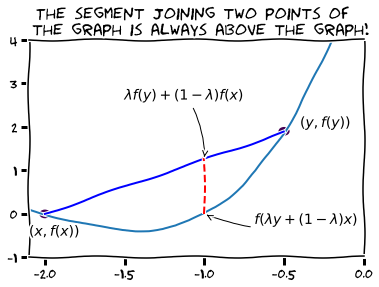
\includegraphics[width=0.5\linewidth]{images/convexFunction1.png} &
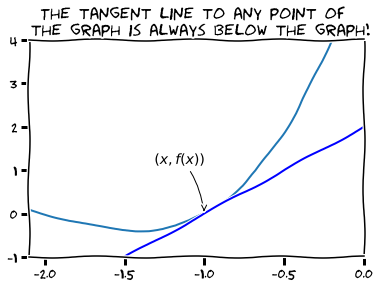
\includegraphics[width=0.5\linewidth]{images/convexFunction2.png}
\end{tabular}
\caption{Convex Functions.}
\label{figure:convexFunction}
\end{figure}
\end{remark}

Two more useful characterization of convex functions.
\begin{theorem}\label{theorem:Hess4Convex}
Suppose that $f\colon C \to \field{R}$ is a function with second partial derivatives on an open convex set $C \subseteq \field{R}^d$.  If the Hessian is positive semidefinite (resp.~positive definite) on $C$, then $f$ is convex (resp.~strictly convex).
\end{theorem}

\begin{theorem}\label{theorem:convexFunctionConvos}
Let $C \subseteq \field{R}^d$ be a convex set.
\begin{enumerate}
	\item \label{theorem:convexFunctionConvo1} If $f_k \colon C \to \field{R}$ are convex functions for $1\leq k \leq n$, then so is the sum $f \colon C \to \field{R}$:
	\begin{equation*}
	f(\x) = \sum_{k=1}^n f_k(\x).
	\end{equation*}  
	If at least one of them is strictly convex, then so is $f$.
	\item \label{theorem:convexFunctionConvo2} If $f \colon C \to \field{R}$ is convex (resp.~strictly convex) on $C$, then so is $\lambda f$ for any $\lambda > 0$.
	\item \label{theorem:convexFunctionConvo3} If $f \colon C \to \field{R}$ is convex (resp.~strictly convex) on $C$, and $g\colon f(C) \to \field{R}$ is an increasing convex function (resp.~strictly increasing convex), then so is $g\circ f$.
	\item \label{theorem:convexFunctionConvo4} If $f,g\colon C \to \field{R}$ are convex functions on $C$, then so is $\max\{ f,g \}$.
\end{enumerate}
\end{theorem}

\begin{example}
Consider the function $f(x,y,z)$ defined on $\field{R}^3$ by
\begin{equation*}
f(x,y,z) = 2x^2+y^2+z^2+2yz.
\end{equation*}
Notice that for all $(x,y,z) \in \field{R}^3$,
\begin{align*}
\Hess{f}(x,y,z) &= \begin{bmatrix} 4 & 0 & 0 \\ 0 & 2 & 2 \\ 0 & 2 & 2 \end{bmatrix}, & \Delta_1 &= 4 > 0, &\Delta_2 &=8 > 0, &\Delta_3 &=0.
\end{align*}
By virtue of Theorem \ref{theorem:Hess4Convex}, we infer that the function $f$ is convex, but not strictly convex.
\end{example}

\begin{example}
To prove that $f(x,y,z) = e^{x^2+y^2+z^2}$ is convex, rather than computing the Hessian and address if it is positive (semi)definite, it is easier to realize that we can write $f = g\circ h$ with 
\begin{align*}
&g \colon \field{R} \to \field{R} && h \colon \field{R}^3 \to \field{R} \\
& g(x) = e^x && h(x,y,z)=x^2+y^2+z^2
\end{align*}
The function $g$ is trivially strictly increasing and convex (since $g'(x) = g''(x) = e^x > 0$ for all $x \in \field{R}$).  The function $h$ is strictly convex, since (by Theorem \ref{theorem:Hess4Convex})
\begin{align*}
\Hess{h}(x,y,z) &= \begin{bmatrix} 2 & 0 & 0 \\ 0 & 2 & 0 \\ 0 & 0 & 2 \end{bmatrix}, &\Delta_1 &=2 >0, &\Delta_2 &=4 >0, &\Delta_3 &=8 > 0.
\end{align*}
By virtue of \ref{theorem:convexFunctionConvo3} in Theorem \ref{theorem:convexFunctionConvos}, we infer that $f$ is strictly convex.
\end{example}

\begin{example}
Set $C = \{ (x,y) \in \field{R}^2 : x>0, y>0 \}$.  Consider the function $f\colon C \to \field{R}$ given by
\begin{equation*}
f(x,y) = x^2 -4xy+5y^2 - \log (xy)
\end{equation*}
Notice we may write $f = g+h$ with $g,h \colon C \to \field{R}$ given respectively by $g(x,y) = x^2 -4xy+5y^2$ and $h(x,y) = -\log(xy)$.  Note also that both functions are strictly convex, since for all $(x,y) \in C$:
\begin{align*}
\Hess{g}(x,y) &= \begin{bmatrix} 2 & -4 \\ -4 & 10 \end{bmatrix}, &\Delta_1 &= 2 >0, & \Delta_2 &=4 >0, \\
\Hess{h}(x,y) &= \begin{bmatrix} x^{-2} & 0 \\ 0 & y^{-2} \end{bmatrix}, &\Delta_1 &= x^{-2} >0, &\Delta_2 &=(xy)^{-2} >0. 
\end{align*}
By virtue of part \ref{theorem:convexFunctionConvo1} in Theorem \ref{theorem:convexFunctionConvos}, we infer that $f$ is strictly convex.
\end{example}

We are now ready to explore existence and characterization of extrema in a wide variety of situations.

\section{Existence results}
\subsection{Continuous functions on compact domains}
The existence of global extrema is guaranteed for continuous functions over compact sets thanks to the following two basic results:

\begin{theorem}[Bounded Value Theorem]\label{theorem:BVT}\index{Theorem!Bounded Value}
The image $f(K)$ of a continuous real-valued function $f \colon \field{R}^d \to \field{R}$ on a compact set $K$ is bounded: there exists $M>0$ so that $\abs{ f(\x) } \leq M$ for all $\x \in K$.
\end{theorem}

\begin{theorem}[Extreme Value Theorem]\label{theorem:EVT}\index{Theorem!Extreme Value}
A continuous real-valued function $f \colon K \to \field{R}$ on a compact set $K \subset \field{R}^d$ takes on minimal and maximal values on $K$.
\end{theorem}

\subsection{Continuous functions on unbounded domains}
Extra restrictions must be applied to the behavior of $f$ in this case, if we want to guarantee the existence of extrema. 

\begin{theorem}\label{theorem:CoerciveFunctions}\index{Function!coercive}
Coercive functions always have a global minimum.
\end{theorem}
\begin{proof}
Since $f$ is coercive, there exists $r>0$ so that $f(\x) > f(\boldsymbol{0})$ for all $\x$ satisfying $\norm{\x}>r$.  On the other hand, consider the closed ball $K_r = \{ \x \in \field{R}^2 : \norm{\x} \leq r \}$.  The continuity of $f$ guarantees a global minimum $\xstar \in K_r$ with $f(\xstar) \leq f(\boldsymbol{0})$.  It is then $f(\xstar) \leq f(\x)$ for all $\x \in \field{R}^d$ trivially.
\end{proof}

\section{Characterization results}

Differentiability is key to guarantee characterization of extrema.  Critical points lead the way:

\begin{theorem}[First order necessary optimality condition for minimization]\label{theorem:criticalGivesMinima}
Suppose $f\colon \field{R}^d \to \field{R}$ is differentiable at $\xstar$.  If $\xstar$ is a local minimum, then $\gradient{f}(\xstar)=0$.
\end{theorem}

To be able to classify extrema of a properly differentiable function, we take into account the behavior of the function around $f(\x)$ with respect to the tangent hyperplane at the point $\big(\x, f(\x)\big)$.  Second derivatives make this process very easy.

\begin{theorem}\label{theorem:coerciveMinima}
Suppose $f \colon \field{R}^d \to \field{R}$ is coercive and continuously differentiable at a point $\xstar$.  If $\xstar$ is a global minimum, then $\gradient{f}(\xstar)= \boldsymbol{0}$.
\end{theorem}

\begin{theorem}[Second order necessary optimality condition for minimization]\label{theorem:necessaryMinima}
Suppose that $f\colon \field{R}^d \to \field{R}$ is twice continuously differentiable at $\xstar$.  
\begin{itemize}
\item If $\xstar$ is a local minimum, then $\gradient{f}(\xstar)=0$ and $\Hess{f}(\xstar)$ is \emph{positive semidefinite}.
\item If $\xstar$ is a strict local minimum, then $\gradient{f}(\xstar)=0$ and $\Hess{f}(\xstar)$ is \emph{positive definite}.
\end{itemize}
\end{theorem}

\begin{theorem}[Second order sufficient optimality conditions for minimization]\label{theorem:sufficientMinima}
Suppose $f\colon D \subseteq \field{R}^d \to \field{R}$ is twice continuously differentiable at a point $\xstar$ in the interior of $D$ and $\gradient{f}(\xstar)=0$.  Then $\xstar$ is a:
\begin{description}
	\item[Local Minimum] if $\Hess{f}(\xstar)$ is \emph{positive semidefinite}.
	\item[Strict Local Minimum] if $\Hess{f}(\xstar)$ is \emph{positive definite}.
\end{description}
If $D=\field{R}^d$ and $\xstar \in \field{R}^d$ satisfies $\gradient{f}(\xstar)=0$, then $\xstar$ is a:
\begin{description}
	\item[Global Minimum] if $\Hess{f}(\x)$ is \emph{positive semidefinite} for all $\x \in \field{R}^d$.
	\item[Strict Global Minimum] if $\Hess{f}(\x)$ is \emph{positive definite} for all $\x \in \field{R}^d$.
\end{description}
\end{theorem}

\begin{theorem}\label{theorem:ConvexMinima}\index{Function!convex}\index{Function!strictly convex}
Any local minimum of a convex function $f\colon C \to \field{R}$ on a convex set $C \subseteq \field{R}^d$ is also a global minimum.  If $f$ is a strictly convex function, then any local minimum is the unique strict global minimum.
\end{theorem}

\begin{theorem}\label{theorem:ConvexCritical}\index{Function!convex}
Suppose $f\colon C \to \field{R}$ is a convex function with continuous first partial derivatives on a convex set $C \subseteq \field{R}^d$.  Then, any critical point of $f$ in $C$ is a global minimum of $f$.
\end{theorem}

\section*{Examples}

\begin{example}
Find a global minimum in $\field{R}^3$ (if it exists) for the function 
\begin{equation*}
f(x,y,z)=e^{x-y} + e^{y-x} + e^{x^2}+z^2.
\end{equation*}
This function has continuous partial derivatives of any order in $\field{R}^3$. Its continuity does not guarantee existence of a global minimum initially since the domain is not compact, but we may try our luck with its critical points.  Note $\gradient{f}(x,y,z) = \big[ e^{x-y} - e^{y-x} + 2xe^{x^2}, -e^{x-y}+e^{y-x}, 2x \big]$.  The only critical point is then $(0,0,0)$ (Why?). The Hessian at that point is positive definite:
\begin{align*}
&&\Hess{f}(0,0,0) &= \begin{bmatrix} 4 & -2 & 0 \\ -2 & 2 & 0 \\ 0 & 0 & 2 \end{bmatrix}, &
\Delta_1 &= 4 > 0, & \Delta_2 &= 4 >0, &\Delta_3 &= 8 > 0.
\end{align*}
By Theorem \ref{theorem:sufficientMinima}, $f(0,0,0)=3$ is a priori a strict local global minimum value.  To prove that this point is actually a strict global minimum, notice that 
\begin{equation*}
\Hess{f}(x,y,z)= \begin{bmatrix} 
e^{x-y}+e^{y-x}+4x^2e^{x^2}+2e^{x^2} & -e^{x-y}-e^{y-x} & 0 \\
-e^{x-y}-e^{y-x} & e^{x-y}+e^{y-x} & 0 \\
0 & 0 & 2 
\end{bmatrix}
\end{equation*}
The first principal minor is trivially positive: $\Delta_1 = e^{x-y}+e^{y-x}+4x^2e^{x^2}+2e^{x^2}$, since it is a sum of three positive terms and on non-negative term.  The second principal minor is also positive:
\begin{align*}
\Delta_2 &= \det \begin{bmatrix} e^{x-y}+e^{y-x}+4x^2e^{x^2}+2e^{x^2} & -e^{x-y}-e^{y-x} \\ -e^{x-y}-e^{y-x} & e^{x-y}+e^{y-x} \end{bmatrix} \\
&= (e^{x-y}+e^{y-x})^2 + (e^{x-y}+e^{y-x})(4x^2e^{x^2}+2e^{x^2}) - (e^{x-y}+e^{y-x})^2 \\
&= (e^{x-y}+e^{y-x})(4x^2e^{x^2}+2e^{x^2}) > 0 
\end{align*}
The third principal minor is positive too: $\Delta_3 = 2\Delta_2 > 0$.  We have just proved that $\Hess{f}(x,y,z)$ is positive definite for all $(x,y,z) \in \field{R}^3$, and thus $(0,0,0)$ is a strict global minimum.
\end{example}

\begin{example}
Find global minima in $\field{R}^2$ (if they exist) for the function
\begin{equation*}
f(x,y) = e^{x-y} + e^{y-x}.
\end{equation*}
This function also has continuous partial derivatives of any order, but no extrema is guaranteed a priori.  Notice that all points $(x, y)$ satisfying $y = x$ are critical.  For such points, the corresponding Hessians and principal minors are given by
\begin{align*}
\Hess{f}(x,x) &= \begin{bmatrix} 2 & -2 \\ -2 & 2 \end{bmatrix}, & \Delta_1 &= 2 >0, & \Delta_2 &= 0;
\end{align*}
therefore, $\Hess{f}(x,x)$ is positive semidefinite for each critical point.  By Theorem \ref{theorem:sufficientMinima}, $f(x,x) = 2$ is a local minimum for all $x \in \field{R}$.  To prove they are global minima, notice that for each $(x,y) \in \field{R}^2$:
\begin{align*}
\Hess{f}(x,y) &= \begin{bmatrix} e^{x-y}+e^{y-x} & -e^{x-y}-e^{y-x} \\ -e^{x-y} - e^{y-x} & e^{x-y}+e^{y-x} \end{bmatrix}, \\
\Delta_1 &= e^{x-y}+e^{y-x} > 0, \quad \Delta_2 =0.
\end{align*}
The Hessian is positive semidefinite for all points, hence proving that any point in the line $y=x$ is a global minimum of $f$.
\end{example}

\begin{example}
Find local and global minima in $\field{R}^2$ (if they exist) for the function 
\begin{equation*}
f(x,y) = x^3-12xy+8y^3.
\end{equation*}
This is a polynomial of degree 3, so we have continuous partial derivatives of any order.  It is easy to see that this function has no global minima: 
\begin{equation*}
\lim_{x\to -\infty} f(x,0) = \lim_{x\to -\infty} x^3 = -\infty.
\end{equation*}
Let's search instead for local minima.  From the equation $\gradient{f}(x,y)=\boldsymbol{0}$ we obtain two critical points: $(0,0)$ and $(2,1)$.  The corresponding Hessians and their eigenvalues are:
\begin{align*}
\Hess{f}(0,0) &= \begin{bmatrix} 0 & -12 \\ -12 & 0 \end{bmatrix}, &\lambda_1 &=-12<0, \quad \lambda_2 =12>0 ,\\
\Hess{f}(2,1) &= \begin{bmatrix} 12 & -12 \\ -12 & 48 \end{bmatrix}, &\lambda_1 &= 30-6\sqrt{13}>0, \quad \lambda_2 = 30 + 6\sqrt{30}>0 .
\end{align*}
By Theorem \ref{theorem:sufficientMinima}, we have that $f(2,1)=-8$ is a local minimum, but $f(0,0)=0$ is not.
\end{example}

\begin{example}
Find local and global minima in $\field{R}^2$ (if they exist) for the function
\begin{equation*}
f(x,y) = x^4-4xy+y^4.
\end{equation*}
This is a polynomial of degree 4, so we do have continuous partial derivatives of any order.  There are three critical points: $(0,0)$, $(-1,-1)$ and $(1,1)$.  The latter two are both strict local minima (by virtue of Theorem \ref{theorem:sufficientMinima}).
\begin{align*}
\Hess{f}(-1,-1) = \Hess{f}(1,1) &= \begin{bmatrix} 12 & -4 \\ -4 & 12 \end{bmatrix}, &\Delta_1 &= 12 > 0, & \Delta_2 &= 128 > 0.
\end{align*}
We proved in Example \ref{example:CoerciveFunctionsGeneral} that $f$ is coercive.  By Theorems \ref{theorem:CoerciveFunctions} and \ref{theorem:coerciveMinima} we have that $f(-1,-1)=f(1,1)=-2$ must be strict global minimum values.
\end{example}

\begin{example}
Find local and global minima in $\field{R}^2$ (if they exist) for the function
\begin{equation*}
f(x,y) = 2x^2+y^2 + \frac{1}{2x^2+y^2}.
\end{equation*}
The simplest way is to realize that $f$ is a convex function on $\field{R}^2$.  We prove this by re-writing $f=g\circ h$ as a composition of $g(x) = x+1/x$ on $(0,\infty)$ with $h(x,y) = 2x^2+y^2$ on $\field{R}^2$.  Note that both functions are strictly convex (Why?).

The only critical point of $g$ in $(0,\infty)$ lies at $x=1$.  By Theorem \ref{theorem:ConvexCritical}, $g(1)=2$ must be a strict global minimum value of $g$.  That being the case, any point $(x,y)$ satisfying $h(x,y)=1$ is a global minimum of $f$.  These are all the points on the ellipse $2x^2+y^2=1$. 
\end{example}
%!TEX root = notes.tex

% Continuous and Differentiable functions.  Symmetric matrices

\section*{Exercises}
\begin{problem}[Basic]
Consider the function
\begin{equation*}
f(x,y) = \dfrac{x+y}{2+\cos x}
\end{equation*}
At what points $(x,y) \in \field{R}^2$ is this function continuous?
\end{problem}

\begin{problem}[Intermediate]
Give an example of a $2 \times 2$ symmetric matrix of each kind below:
\begin{enumerate}
	\item positive definite, 
	\item positive semidefinite, 
	\item negative definite, 
	\item negative semidefinite,
	\item indefinite.
\end{enumerate}
\end{problem}

\begin{problem}[Basic]\cite[p.31, \#2]{peressini1988mathematics}
Classify the following matrices according to whether they are positive or negative definite or semidefinite or indefinite:
\begin{align*}
\mathrm{(a)} & \begin{bmatrix} 1 & 0 & 0 \\ 0 & 3 & 0 \\ 0 & 0 & 5 \end{bmatrix}  &
\mathrm{(b)} & \begin{bmatrix} -1 & 0 & 0 \\ 0 & -3 & 0 \\ 0 & 0 & -2 \end{bmatrix} &
\mathrm{(c)} & \begin{bmatrix} 7 & 0 & 0 \\ 0 & -8 & 0 \\ 0 & 0 & 5 \end{bmatrix}  \\
\mathrm{(d)} & \begin{bmatrix} 3 & 1 & 2 \\ 1 & 5 & 3 \\ 2 & 3 & 7 \end{bmatrix}  &
\mathrm{(e)} & \begin{bmatrix} -4 & 0 & 1 \\ 0 & -3 & 2 \\ 1 & 2 & -5 \end{bmatrix}  &
\mathrm{(f)} & \begin{bmatrix} 2 & -4 & 0 \\ -4 & 8 & 0 \\ 0 & 0 & -3 \end{bmatrix} 
\end{align*}
\end{problem}

\begin{problem}[Basic]\cite[p.31, \#3]{peressini1988mathematics}
Write the quadratic form $\quadratic{A}(\x)$ associated with each of the following matrices $\boldsymbol{A}$:
\begin{align*}
\mathrm{(a)} & \begin{bmatrix} -1 & 2 \\ 2 & 3 \end{bmatrix} &
\mathrm{(b)} & \begin{bmatrix} 1 & -1 & 0 \\ -1 & -2 & 2 \\ 0 & 2 & 3 \end{bmatrix} \\
\mathrm{(c)} & \begin{bmatrix} 2 & -3 \\ -3 & 0 \end{bmatrix} &
\mathrm{(d)} & \begin{bmatrix} -3 & 1 & 2 \\ 1 & 2 & -1 \\ 2 & -1 & 4 \end{bmatrix} \\
\end{align*}
\end{problem}

\begin{problem}[Basic]\cite[p.32, \#4]{peressini1988mathematics}
Write each of the quadratic forms below in the form $\x \boldsymbol{A} \transpose{\x}$ for an appropriate symmetric matrix $\boldsymbol{A}$:
\begin{enumerate}
\item $3x^2-xy+2y^2$.
\item $x^2+2y^2-3z^2+2xy-4xz+6yz$.
\item $2x^2-4z^2+xy-yz$.
\end{enumerate}
\end{problem}

% Coercive Functions

\begin{problem}[Intermediate]
Identify which of the following real-valued functions are coercive.  Explain the reason.
\begin{enumerate}
	\item $f(x,y) = \sqrt{x^2+y^2}$.
	\item $f(x,y) = x^2 + 9y^2 - 6xy$.
	\item $f(x,y) = x^4 - 3xy +y^4$.
	\item Rosenbrock functions $\mathcal{R}_{a,b}$.
\end{enumerate}
\end{problem}

\begin{problem}[Advanced]\cite[p.36, \#32]{peressini1988mathematics}
Find an example of a continuous, real-valued, non-coercive function $f\colon \field{R}^2 \to \field{R}$ that satisfies, for all $t \in \field{R}$,
\begin{equation*}
\lim_{x \to \infty} f(x, tx) = \lim_{y \to \infty} f(ty, y) = \infty.
\end{equation*}
\end{problem}

% Convex functions

\begin{problem}[Basic]\cite[p.77, \#1,2,7]{peressini1988mathematics}
Determine whether the given functions are convex, concave, strictly convex or strictly concave on the specified domains:
\begin{enumerate}
	\item $f(x) = \log(x)$ on $(0,\infty)$.
	\item $f(x) = e^{-x}$ on $\field{R}$.
	\item $f(x) = \abs{x}$ on $[-1,1]$.
	\item $f(x) = \abs{x^3}$ on $\field{R}$.
	\item $f(x,y) = 5x^2+2xy+y^2-x+2x+3$ on $\field{R}^2$.
	\item $f(x,y) = x^2/2+3y^2/2+\sqrt{3}xy$ on $\field{R}^2$.
	\item $f(x,y) = 4e^{3x-y}+5e^{x^2+y^2}$ on $\field{R}^2$.
	\item $f(x,y,z) = x^{1/2} + y^{1/3} + z^{1/5}$ on $C = \{ (x,y,z) : x>0, y>0, z>0 \}$.
\end{enumerate}
\end{problem}

\begin{problem}[Intermediate]\cite[p.79 \#11]{peressini1988mathematics}
Sketch the epigraph of the following functions
\begin{enumerate}
	\item $f(x) = e^x$.
	\item $f(x,y)=x^2+y^2$.
\end{enumerate}
\end{problem}

% Existence

\begin{problem}[Intermediate]
For the following optimization problems, state whether existence of a solution is guaranteed:
\begin{enumerate}
	\item $f(x) = (1+x)/x$ over $[1,\infty)$
	\item $f(x) = 1/x$ over $[1,2)$
	\item The following piecewise function over $[1,2]$
	\begin{equation*}
	f(x) = \begin{cases}
	1/x, &1\leq x<2 \\
	1,   &x=2
	\end{cases}
	\end{equation*}
\end{enumerate}
\end{problem}

% Characterization

\begin{problem}[Advanced]
State and prove equivalent results to Theorems \ref{theorem:criticalGivesMinima}, \ref{theorem:necessaryMinima} and \ref{theorem:sufficientMinima} to describe necessary and sufficient conditions for the characterization of \emph{maxima}.
\end{problem}

\begin{problem}[Basic]\cite[p.32, \#7]{peressini1988mathematics}
Use the \emph{Principal Minor Criteria} (Theorem \ref{theorem:PrincipalMinors}) to determine---if possible---the nature of the critical points of the following functions:
\begin{enumerate}
	\item $f(x,y) = x^3+y^3-3x-12y+20$.
	\item $f(x,y,z) = 3x^2+2y^2+2z^2+2xy+2yz+2xz$.
	\item $f(x,y,z) = x^2+y^2+z^2-4xy$.
	\item $f(x,y) = x^4+y^4-x^2-y^2+1$.
	\item $f(x,y) = 12x^3+36xy-2y^3+9y^2-72x+60y+5$.
\end{enumerate}
\end{problem}

% \begin{problem}\cite[p.35 \#26]{peressini1988mathematics}
% Show that the function 
% \begin{equation*}
% f(x,y,z) = e^{x^2+y^2+z^2}-x^4-y^6-z^6
% \end{equation*} 
% has a global minimum on $\field{R}^3$.
% \end{problem}

\begin{problem}[Intermediate]\cite[p.36 \#33]{peressini1988mathematics}
Consider the function
\begin{equation*}
f(x,y) = x^3 + e^{3y} -3xe^y.
\end{equation*}
Show that $f$ has exactly one critical point, and that this point is a local minimum but not a global minimum.
\end{problem}

\begin{problem}[Basic]
Let $f(x,y) = -\log(1-x-y)-\log x -\log y$.
\begin{enumerate}
	\item Find the domain $D$ of $f$.
	\item Prove that $D$ is a convex set.
	\item Prove that $f$ is strictly convex on $D$.
	\item Find the strict global minimum.
\end{enumerate}
\end{problem}

\begin{problem}[Basic]\cite[p.81 \#27]{peressini1988mathematics}
Find local and global minima in $\field{R}^3$ (if they exist) for the function 
\begin{equation*}
f(x,y) = e^{x+z-y}+e^{y-x-z}
\end{equation*}
\end{problem}



%%%%% chapter 3
\chapter{Numerical Approximation for Unconstrained Optimization}\label{chapter:UnconstrainedNumerical}
%!TEX root = notes.tex

\chapter{Numerical Approximation for Unconstrained Optimization}\label{chapter:nonlinearoptimization}
Although technically any characterization result finds the exact value of the extrema of a function, computationally this is hardly feasible (specially for functions of very high dimension).  See the following session based on problem \ref{problem:tricky} for an example, where we try to find the critical points of the function $f(x,y,z)=e^{x^2+y^2+z^2}-x^4-y^y-z^6$ symbolically in Python with the \texttt{sympy} libraries:

% framesep=2mm,
% baselinestretch=1.2,
\begin{minted}[frame=single, fontsize=\footnotesize, linenos ]{python}
# Importing necessary symbols/libraries/functions
from sympy.abc import x,y,z
from sympy import Matrix, solve, exp
from sympy.tensor.array import derive_by_array

# Description of f, computation of its gradient and Hessian
f = exp(x**2 + y**2 + z**2) - x**4 -y**6 - z**6
gradient = derive_by_array(f, [x,y,z])
hessian  = Matrix([derive_by_array(gradient, a) for a in [x,y,z]])
\end{minted}
While the correct expressions for $\gradient{f}$ and $\Hess{f}$ are quickly computed, trying to find critical points results in an error:
\begin{minted}[frame=single,fontsize=\footnotesize, linenos, firstnumber=10,mathescape]{python}
# Search of critical points by solving $\gradient{f}=0$
solve(gradient)
\end{minted}

\begin{minted}[frame=lines,fontsize=\footnotesize]{python}
NotImplementedError: could not solve 
4*x**2*sqrt(-log(exp(x**2)/(2*x**2))) - 6*(-log(exp(x**2)/(2*x**2)))**(5/2)
\end{minted}

Too complex a task to be performed symbolically, although the obvious answer is $(0,0,0)$.  A better way to approach this is by trying to approximate this minimum using the structure of the graph of $f$.  In these notes we are going to explore several strategies to accomplish this task, based on the concept of \emph{iterative methods for finding zeros of real-valued functions}.

\begin{example}[The Newton-Raphson method]
In order to find a many correct decimal places of $\sqrt{2}$, we allow a computer to find better and better approximations of the solution of the equation $f(x)=x^2-2$.  We start with a decent guess, say $x_0=3$.  We construct a sequence $\{ x_n \}_{n\in\field{N}}$ that converges to $\sqrt{2}$ as follows:
\begin{enumerate}
\item Find the tangent line to the graph of $f$ at $x_0$, 
\begin{equation*}
y-f(x_0)=f'(x_0)(x-x_0)
\end{equation*}
\item Provided this line is not horizontal ($f'(x_0)\neq 0$), report the intersection of this line with the $x$--axis.  Call this intersection $x_1$
\begin{equation*}
x_1=x_0-\frac{f(x_0)}{f'(x_0)}
\end{equation*}
\item Repeat this process, to get the sequence 
\begin{equation*}
x_{n+1} = x_n- \frac{f(x_n)}{f'(x_n)}
\end{equation*}
\end{enumerate}
\begin{figure}[ht!]
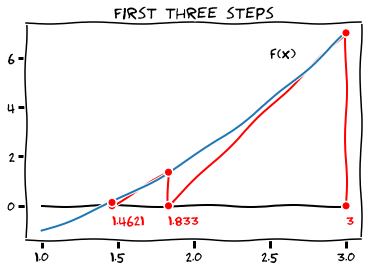
\includegraphics[width=0.65\linewidth]{newton1.png}
\caption{Newton-Raphson iterative method}
\label{figure:Newton-Raphson}
\end{figure}
Note the result of applying this process a few times:

\begin{table}[ht!]
\begin{tabular}{|c|c|r|} \hline 
$n$ & $x_n$ & $f(x_n)$ \\ \hline \hline 
$0$ & $3.000000000000000$ & $7.0000E+00$ \\ \hline 
$1$ & $1.833333333333333$ & $1.3611E+00$ \\ \hline 
$2$ & $1.462121212121212$ & $1.3780E-01$ \\ \hline 
$3$ & $1.414998429894803$ & $2.2206E-03$ \\ \hline 
$4$ & $1.414213780047198$ & $6.1568E-07$ \\ \hline 
$5$ & $1.414213562373112$ & $4.7518E-14$ \\ \hline 
$6$ & $1.414213562373095$ & $-4.4409E-16$ \\ \hline 
$7$ & $1.414213562373095$ & $4.4409E-16$ \\ \hline 
\end{tabular}
\caption{Convergence to $\sqrt{2}$ with 15-digit accuracy in 6 steps}
\label{table:Newton-Raphson}
\end{table}
\end{example}

Let's proceed to extend this process to functions $\boldsymbol{g} \colon \field{R}^d \to \field{R}^d$ as follows.  
\begin{itemize}
	\item Any function $\boldsymbol{g} \colon \field{R}^d \to \field{R}^d$ can be described in the form $\boldsymbol{g}(\x) = \big( g_1(\x), g_2(\x), \dotsc, g_d(\x) \big)$ for $d$ real-valued functions $g_k\colon \field{R}^d \to \field{R}$ ($1\leq k \leq d$).
	\item For such a function $\boldsymbol{g}$, we may express its gradient as a $d\times d$ matrix in the form
	\begin{equation*}
	\gradient{\boldsymbol{g}} = \begin{bmatrix}
	\frac{\partial g_1}{\partial x_1} & \frac{\partial g_1}{\partial x_2} & \dotsb & \frac{\partial g_1}{\partial x_d} \\ \\
	\frac{\partial g_2}{\partial x_1} & \frac{\partial g_2}{\partial x_2} & \dotsb & \frac{\partial g_2}{\partial x_d} \\ \\
	\vdots & \vdots & \ddots & \vdots \\ \\
	\frac{\partial g_d}{\partial x_1} & \frac{\partial g_d}{\partial x_2} & \dotsb & \frac{\partial g_d}{\partial x_d} \\
	\end{bmatrix}
	\end{equation*}
\end{itemize}
Start with a guess for the solution, $\x_0$, and on the $n$--th step of the algorithm compute the $(n+1)$--th term of the sequence by
\begin{equation*}
\x_{n+1} = \x_n - \big[ \gradient{\boldsymbol{g}}(\x_n) \big]^{-1} \boldsymbol{g}(\x_n),
\end{equation*}
where $\big[ \gradient{\boldsymbol{g}}(\x_n) \big]^{-1}$ represents the inverse matrix of the gradient at $\x_n$.  This is equivalent to selecting in the tangent hyperplane to the graph of $\boldsymbol{g}$ at $\boldsymbol{g}(\x_n)$, the one line in the direction with the most rapid increase/decrease.  The computation of $\x_{n+1}$ is therefore the intersection of that line with the hyperplane $x_d=0$.

\begin{example}\label{example:preNewton4poly4}
Consider the function $\boldsymbol{g}\colon \field{R}^2 \to \field{R}^2$ given by
\begin{equation*}
\boldsymbol{g}(x,y,z) = \big( x^3-y, y^3-x \big)
\end{equation*}
Its gradient at each $(x,y)$ is given by
\begin{equation*}
\gradient{\boldsymbol{g}}(x,y) = \begin{bmatrix} 3x^2 & -1 \\ -1 & 3y^2 \end{bmatrix}
\end{equation*}
Note the determinant of this matrix is $\det \gradient{\boldsymbol{g}}(x,y) = 9x^2y^2-1 = (3xy-1)(3xy+1)$.  For any point $(x,y)$ that does not make this expression zero, this is an invertible matrix with 
\begin{equation*}
\big[ \gradient{\boldsymbol{g}}(x,y)\big]^{-1} = \frac{1}{9x^2y^2-1}\begin{bmatrix} 3y^2 & 1 \\ 1 & 3x^2 \end{bmatrix}
\end{equation*}
For a decent guess $(x_0, y_0)$, the sequence computed by the Newton method is then given by
\begin{align*}
\begin{bmatrix} x_{n+1} \\ y_{n+1} \end{bmatrix} &= \begin{bmatrix} x_n \\ y_n \end{bmatrix} -\frac{1}{9 x_n^2 y_n^2-1}\begin{bmatrix} 3y_n^2 & 1 \\ 1 & 3x_n^2 \end{bmatrix} \begin{bmatrix} x_n^3-y_n \\ y_n^3-x_n \end{bmatrix} \\
&= \begin{bmatrix}
x_n - \frac{3x_n^3 y_n^2-2 y_n^3-x_n}{9x_n^2  y_n^2-1} \\  y_n - \frac{3x_n^2 y_n^3+-2x_n^3- y_n}{9x_n^2 y_n^2-1}
\end{bmatrix}
\end{align*}
Let's run this process with three different initial guesses:
\begin{enumerate}
	\item Starting at $(x_0, y_0) = (-1.0,1.0)$, the sequence converges to $(0,0)$.  %See Table \ref{table:00}.
	\begin{table}[ht!]
	\begin{tabular}{|c|c|c|} \hline 
	$n$ & $x_n$ & $y_n$ \\ \hline \hline 
	$0$ & $-1.00000000$ & $1.00000000$ \\ \hline 
	$1$ & $-0.50000000$ & $0.50000000$ \\ \hline 
	$2$ & $-0.14285714$ & $0.14285714$ \\ \hline 
	$3$ & $-0.00549451$ & $0.00549451$ \\ \hline 
	$4$ & $-0.00000033$ & $0.00000033$ \\ \hline 
	$5$ & $-0.00000000$ & $0.00000000$ \\ \hline 
	$6$ & $-0.00000000$ & $0.00000000$ \\ \hline 
	\end{tabular}
	\caption{Convergence to $(0,0)$ in 5 steps}
	\label{table:00}
	\end{table}
	\item Starting at $(x_0,y_0) = (3.5, 2.1)$, the sequence converges to $(1,1)$.  %See Table \ref{table:11}.
	\begin{table}[ht!]
	\begin{tabular}{|c|c|c|} \hline 
	$n$ & $x_n$ & $y_n$ \\ \hline \hline 
	$0$ & $3.50000000$ & $2.10000000$ \\ \hline 
	$1$ & $2.37631607$ & $1.57961573$ \\ \hline 
	$2$ & $1.65945969$ & $1.27476534$ \\ \hline 
	$3$ & $1.23996276$ & $1.10419072$ \\ \hline 
	$4$ & $1.04837462$ & $1.02274752$ \\ \hline 
	$5$ & $1.00260153$ & $1.00133122$ \\ \hline 
	$6$ & $1.00000824$ & $1.00000451$ \\ \hline 
	$7$ & $1.00000000$ & $1.00000000$ \\ \hline 
	$8$ & $1.00000000$ & $1.00000000$ \\ \hline 
	\end{tabular}
	\caption{Convergence to $(1,1)$ in 7 steps}
	\label{table:11}
	\end{table}
	\item Starting at $(x_0, y_0) = (-13.5, -7.3)$, the sequence converges to $(-1,-1)$.  %See Table \ref{table:-1-1}.
	\begin{table}[ht!]
	\begin{tabular}{|c|c|c|} \hline 
	$n$ & $x_n$ & $y_n$ \\ \hline \hline 
	$0$ & $-13.50000000$ & $-7.30000000$ \\ \hline 
	$1$ & $-9.00900415$ & $-4.92301873$ \\ \hline 
	$2$ & $-6.01982204$ & $-3.36480659$ \\ \hline 
	$3$ & $-4.03494126$ & $-2.36199873$ \\ \hline 
	$4$ & $-2.72553474$ & $-1.73750959$ \\ \hline 
	$5$ & $-1.87830623$ & $-1.36573112$ \\ \hline 
	$6$ & $-1.36121191$ & $-1.15374930$ \\ \hline 
	\end{tabular}
	\begin{tabular}{|c|c|c|} \hline 
	$n$ & $x_n$ & $y_n$ \\ \hline \hline 
	$7$ & $-1.09518303$ & $-1.04341362$ \\ \hline 
	$8$ & $-1.00932090$ & $-1.00463507$ \\ \hline 
	$9$ & $-1.00010404$ & $-1.00005571$ \\ \hline 
	$10$ & $-1.00000001$ & $-1.00000001$ \\ \hline 
	$11$ & $-1.00000000$ & $-1.00000000$ \\ \hline 
	$12$ & $-1.00000000$ & $-1.00000000$ \\ \hline 
	$13$ & $-1.00000000$ & $-1.00000000$ \\ \hline 
	\end{tabular}
	\caption{Convergence to $(-1,-1)$ in 11 steps}
	\label{table:-1-1}
	\end{table}
\end{enumerate}
\end{example}

We can readily see how this process aids in the computation of critical points of a real-valued function $f\colon \field{R}^d \to \field{R}$:
\begin{enumerate}
	\item Set $\boldsymbol{g}(\x) = \gradient{f}(\x) = \big[ \frac{\partial f}{\partial x_1}, \dotsc, \frac{\partial f}{\partial x_d} \big]$
	\item It is then $\gradient{\boldsymbol{g}}(\x) = \Hess{f}(\x)$
	\item Perform a Newton method with a decent initial guess $\x_0$ on $\boldsymbol{g}=\gradient{f}$ to obtain the sequence
	\begin{equation*}
	\x_{n+1} = \x_n - \big[ \Hess{f}(\x_n) \big]^{-1} \cdot \gradient{f}(\x_n)
	\end{equation*}
\end{enumerate}

\begin{example}
Consider the function $f(x,y) = x^4-4xy+y^4$ over $\field{R}^2$.  Notice $\gradient{f}(x,y) = \big( x^3-y, y^3-x \big)$, as function $\boldsymbol{g}$ in Example \ref{example:preNewton4poly4}.  The critical points we found were $(0,0)$, $(-1,-1)$ and $(1,1)$.
\end{example}
\begin{example}
A similar process for the Rosenbrock function $\mathcal{R}_{1,1}(x,y) = (1-x)^2 + (y-x^2)^2$ gives the following recurrence formula:
\begin{align*}
\begin{bmatrix} x_{n+1} \\ y_{n+1} \end{bmatrix} &=
\begin{bmatrix} x_{n} \\ y_{n} \end{bmatrix} - \big[ \Hess{\mathcal{R}_{1,1}}(x_n,y_n) \big]^{-1} \cdot \gradient{\mathcal{R}_{1,1}}(x_n, y_n) \\
&= \begin{bmatrix} x_{n} \\ y_{n} \end{bmatrix} - \frac{2}{2x^2-2y+1} \begin{bmatrix}
1/2 & x \\ x & 6x^2-2y+1
\end{bmatrix} \begin{bmatrix}
2x^3-2xy+x-1 \\ y-x^2
\end{bmatrix} \\
&= \frac{1}{2x^2-2y+1} \begin{bmatrix}
2x^3-2xy+1 \\ x(2x^3-2xy-x+2)
\end{bmatrix}
\end{align*}
Starting with initial guess $(x_0, y_0) = (-2,2)$, the sequence converges to the critical point $(1,1)$.  
\end{example}
\begin{figure}[ht!]
\begin{tabular}{cc}
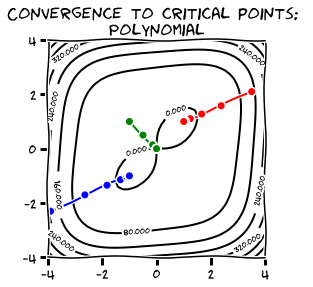
\includegraphics[width=0.45\linewidth]{convergenceNewton.png} &
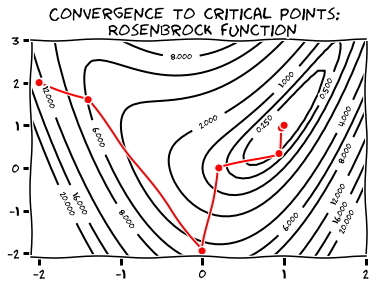
\includegraphics[width=0.55\linewidth]{convergenceNewtonRosenbrock.png} 
\end{tabular}
\caption{Newton method}
\label{figure:NewtonConvergence}
\end{figure}

%!TEX root = notes.tex

\section{Newton's Method}
\begin{example}[The Newton-Raphson method]
In order to find a good estimation of $\sqrt{2}$ with mani decimal places, we allow a computer to find better and better approximations of the solution of the equation $f(x)=x^2-2$.  We start with an initial guess, say $x_0=3$.  We construct a sequence $\{ x_n \}_{n\in\field{N}}$ that converges to $\sqrt{2}$ as follows:
\begin{enumerate}
\item Find the tangent line to the graph of $f$ at $x_0$, 
\begin{equation*}
y-f(x_0)=f'(x_0)(x-x_0)
\end{equation*}
\item Provided this line is not horizontal ($f'(x_0)\neq 0$), report the intersection of this line with the $x$--axis.  Call this intersection $x_1$
\begin{equation*}
x_1=x_0-\frac{f(x_0)}{f'(x_0)}
\end{equation*}
\item Repeat this process, to get the sequence 
\begin{equation*}
x_{n+1} = x_n - \frac{f(x_n)}{f'(x_n)}
\end{equation*}
\end{enumerate}
\begin{figure}[ht!]
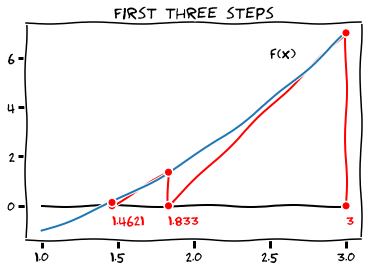
\includegraphics[width=0.65\linewidth]{newton1.png}
\caption{Newton-Raphson iterative method}
\label{figure:Newton-Raphson}
\end{figure}
Note the result of applying this process a few times:

\begin{table}[ht!]
\begin{tabular}{|c|c|r|} \hline 
$n$ & $x_n$ & $f(x_n)$ \\ \hline \hline 
$0$ & $3.000000000000000$ & $7.0000E+00$ \\ \hline 
$1$ & $1.833333333333333$ & $1.3611E+00$ \\ \hline 
$2$ & $1.462121212121212$ & $1.3780E-01$ \\ \hline 
$3$ & $1.414998429894803$ & $2.2206E-03$ \\ \hline 
$4$ & $1.414213780047198$ & $6.1568E-07$ \\ \hline 
$5$ & $1.414213562373112$ & $4.7518E-14$ \\ \hline 
$6$ & $1.414213562373095$ & $-4.4409E-16$ \\ \hline 
$7$ & $1.414213562373095$ & $4.4409E-16$ \\ \hline 
\end{tabular}
\caption{Convergence to $\sqrt{2}$ with 15-digit accuracy in 6 steps}
\label{table:Newton-Raphson}
\end{table}
\end{example}

\begin{example}\label{example:NewtonRaphsonChoice}
Consider now the function $f(x) = 1-\tfrac{1}{x}$ over $(0, \infty)$, which has the obvious root $x=1$. The Newton-Raphson method gives the following iterates for any $x_0 \in (0,\infty)$:
\begin{align*}
x_{n+1} = x_n - \frac{f(x_n)}{f'(x_n)} = x_n \big( 2- x_n \big).
\end{align*}
Notice the two factors in the right-hand side of that expression: $x_n$, and $2-x_n$.  If the initial guess does not satisfy $0<x_0<2$, then the next iteration gives a non-positive value (see Figure \ref{figure:NewtonRaphsonChoice}).  The method will not work on those instances: convergence to a solution is not guaranteed.
\begin{figure}[ht!]
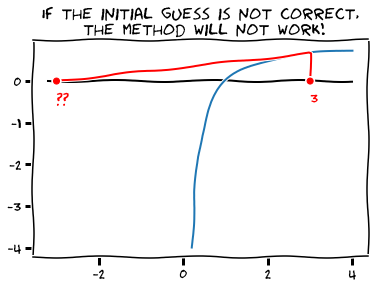
\includegraphics[width=0.65\linewidth]{badNewton.png}
\caption{Initial guess must carefully be chosen in Newton-Raphson}
\label{figure:NewtonRaphsonChoice}
\end{figure}
\end{example}

\begin{example}\label{example:NewtonRaphsonloop}
Consider now $f(x) = \sign(x)\sqrt{\lvert x \rvert}$ over $\field{R}$, with root at $x=0$.  The Newton-Raphson method fails miserably with this function: for any $x_0 \neq 0$
\begin{align*}
x_1 = x_0 - \frac{f(x_0)}{f'(x_0)} = x_0 - \frac{\sign(x_0)\lvert x_0 \rvert^{1/2}}{\tfrac{1}{2}\lvert x_0 \rvert^{-1/2}} = -x_0.
\end{align*}
This sequence turns into a loop: $x_{2n}=x_0$, $x_{2n+1}=-x_0$ for all $n\in \field{N}$ (see Figure \ref{figure:NewtonRaphsonloop}).
\begin{figure}[ht!]
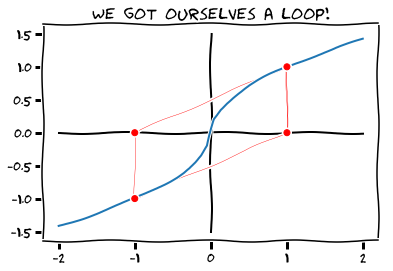
\includegraphics[width=0.65\linewidth]{loop.png}
\caption{Newton-Raphson fails for some functions}
\label{figure:NewtonRaphsonloop}
\end{figure}
\end{example}

Let's proceed to extend this process to functions $\boldsymbol{g} \colon \field{R}^d \to \field{R}^d$ as follows.  
\begin{itemize}
	\item Any function $\boldsymbol{g} \colon \field{R}^d \to \field{R}^d$ can be described in the form $\boldsymbol{g}(\x) = \big[ g_1(\x), g_2(\x), \dotsc, g_d(\x) \big]$ for $d$ real-valued functions $g_k\colon \field{R}^d \to \field{R}$ ($1\leq k \leq d$).
	\item For such a function $\boldsymbol{g}$, we may express its gradient as a $d\times d$ matrix in the form
	\begin{equation*}
	\gradient{\boldsymbol{g}} = \begin{bmatrix}
	\frac{\partial g_1}{\partial x_1} & \frac{\partial g_1}{\partial x_2} & \dotsb & \frac{\partial g_1}{\partial x_d} \\ \\
	\frac{\partial g_2}{\partial x_1} & \frac{\partial g_2}{\partial x_2} & \dotsb & \frac{\partial g_2}{\partial x_d} \\ \\
	\vdots & \vdots & \ddots & \vdots \\ \\
	\frac{\partial g_d}{\partial x_1} & \frac{\partial g_d}{\partial x_2} & \dotsb & \frac{\partial g_d}{\partial x_d} \\
	\end{bmatrix}
	\end{equation*}
\end{itemize}
Start with a guess for the solution, $\x_0$, and on the $n$--th step of the algorithm compute the $(n+1)$--th term of the sequence by
\begin{equation}\label{equation:NewtonMethod}
\x_{n+1} = \x_n - \big[ \gradient{\boldsymbol{g}}(\x_n) \big]^{-1} \boldsymbol{g}(\x_n),
\end{equation}
where $\big[ \gradient{\boldsymbol{g}}(\x_n) \big]^{-1}$ represents the inverse matrix of the gradient at $\x_n$.  This is equivalent to selecting in the tangent hyperplane to the graph of $\boldsymbol{g}$ at $\boldsymbol{g}(\x_n)$, the one line in the direction with the most rapid increase/decrease.  The computation of $\x_{n+1}$ is therefore the intersection of that line with the hyperplane $x_d=0$.  We refer to $\big[ \gradient{\boldsymbol{g}}(\x_n) \big]^{-1} \boldsymbol{g}(\x_n)$ as the \emph{Newton direction} for $\boldsymbol{g}$ at $\x_n$.

\begin{example}\label{example:preNewton4poly4}
Consider the function $\boldsymbol{g}\colon \field{R}^2 \to \field{R}^2$ given by
\begin{equation*}
\boldsymbol{g}(x,y,z) = \big[ x^3-y, y^3-x \big]
\end{equation*}
Its gradient at each $(x,y)$ is given by
\begin{equation*}
\gradient{\boldsymbol{g}}(x,y) = \begin{bmatrix} 3x^2 & -1 \\ -1 & 3y^2 \end{bmatrix}
\end{equation*}
Note the determinant of this matrix is $\det \gradient{\boldsymbol{g}}(x,y) = 9x^2y^2-1 = (3xy-1)(3xy+1)$.  For any point $(x,y)$ that does not make this expression zero, this is an invertible matrix with 
\begin{equation*}
\big[ \gradient{\boldsymbol{g}}(x,y)\big]^{-1} = \frac{1}{9x^2y^2-1}\begin{bmatrix} 3y^2 & 1 \\ 1 & 3x^2 \end{bmatrix}
\end{equation*}
For an initial guess $(x_0, y_0)$, the sequence computed by the Newton method is then given by
\begin{align*}
\begin{bmatrix} x_{n+1} \\ y_{n+1} \end{bmatrix} &= \begin{bmatrix} x_n \\ y_n \end{bmatrix} -\frac{1}{9 x_n^2 y_n^2-1}\begin{bmatrix} 3y_n^2 & 1 \\ 1 & 3x_n^2 \end{bmatrix} \begin{bmatrix} x_n^3-y_n \\ y_n^3-x_n \end{bmatrix} \\
% &= \begin{bmatrix}
% x_n - \frac{3x_n^3 y_n^2-2 y_n^3-x_n}{9x_n^2  y_n^2-1} \\  y_n - \frac{3x_n^2 y_n^3+-2x_n^3- y_n}{9x_n^2 y_n^2-1}
% \end{bmatrix}
\end{align*}
Let's run this process with three different initial guesses:
\begin{enumerate}
	\item Starting at $(x_0, y_0) = (-1.0,1.0)$, the sequence converges to $(0,0)$.  %See Table \ref{table:00}.
	\begin{table}[ht!]
	\begin{tabular}{|c|c|c|} \hline 
	$n$ & $x_n$ & $y_n$ \\ \hline \hline 
	$0$ & $-1.00000000$ & $1.00000000$ \\ \hline 
	$1$ & $-0.50000000$ & $0.50000000$ \\ \hline 
	$2$ & $-0.14285714$ & $0.14285714$ \\ \hline 
	$3$ & $-0.00549451$ & $0.00549451$ \\ \hline 
	$4$ & $-0.00000033$ & $0.00000033$ \\ \hline 
	$5$ & $-0.00000000$ & $0.00000000$ \\ \hline 
	$6$ & $-0.00000000$ & $0.00000000$ \\ \hline 
	\end{tabular}
	\caption{Convergence to $(0,0)$ with 8-digit accuracy in 5 steps}
	\label{table:00}
	\end{table}
	\item Starting at $(x_0,y_0) = (3.5, 2.1)$, the sequence converges to $(1,1)$.  %See Table \ref{table:11}.
	\begin{table}[ht!]
	\begin{tabular}{|c|c|c|} \hline 
	$n$ & $x_n$ & $y_n$ \\ \hline \hline 
	$0$ & $3.50000000$ & $2.10000000$ \\ \hline 
	$1$ & $2.37631607$ & $1.57961573$ \\ \hline 
	$2$ & $1.65945969$ & $1.27476534$ \\ \hline 
	$3$ & $1.23996276$ & $1.10419072$ \\ \hline 
	$4$ & $1.04837462$ & $1.02274752$ \\ \hline 
	$5$ & $1.00260153$ & $1.00133122$ \\ \hline 
	$6$ & $1.00000824$ & $1.00000451$ \\ \hline 
	$7$ & $1.00000000$ & $1.00000000$ \\ \hline 
	$8$ & $1.00000000$ & $1.00000000$ \\ \hline 
	\end{tabular}
	\caption{Convergence to $(1,1)$ with 8-digit accuracy in 7 steps}
	\label{table:11}
	\end{table}
	\item Starting at $(x_0, y_0) = (-13.5, -7.3)$, the sequence converges to $(-1,-1)$.  %See Table \ref{table:-1-1}.
	\begin{table}[ht!]
	\begin{tabular}{|c|c|c|} \hline 
	$n$ & $x_n$ & $y_n$ \\ \hline \hline 
	$0$ & $-13.50000000$ & $-7.30000000$ \\ \hline 
	$1$ & $-9.00900415$ & $-4.92301873$ \\ \hline 
	$2$ & $-6.01982204$ & $-3.36480659$ \\ \hline 
	$3$ & $-4.03494126$ & $-2.36199873$ \\ \hline 
	$4$ & $-2.72553474$ & $-1.73750959$ \\ \hline 
	$5$ & $-1.87830623$ & $-1.36573112$ \\ \hline 
	$6$ & $-1.36121191$ & $-1.15374930$ \\ \hline 
	\end{tabular}
	\begin{tabular}{|c|c|c|} \hline 
	$n$ & $x_n$ & $y_n$ \\ \hline \hline 
	$7$ & $-1.09518303$ & $-1.04341362$ \\ \hline 
	$8$ & $-1.00932090$ & $-1.00463507$ \\ \hline 
	$9$ & $-1.00010404$ & $-1.00005571$ \\ \hline 
	$10$ & $-1.00000001$ & $-1.00000001$ \\ \hline 
	$11$ & $-1.00000000$ & $-1.00000000$ \\ \hline 
	$12$ & $-1.00000000$ & $-1.00000000$ \\ \hline 
	$13$ & $-1.00000000$ & $-1.00000000$ \\ \hline 
	\end{tabular}
	\caption{Convergence to $(-1,-1)$ with 8-digit accuracy in 11 steps}
	\label{table:-1-1}
	\end{table}
\end{enumerate}
\end{example}

We can readily see how this process aids in the computation of critical points of twice continuously differentiable real-valued function $f\colon \field{R}^d \to \field{R}$:
\begin{enumerate}
	\item Set $\boldsymbol{g}(\x) = \gradient{f}(\x) = \big[ \frac{\partial f}{\partial x_1}, \dotsc, \frac{\partial f}{\partial x_d} \big]$
	\item It is then $\gradient{\boldsymbol{g}}(\x) = \Hess{f}(\x)$
	\item Perform a Newton method (with initial guess $\x_0$) on $\boldsymbol{g}=\gradient{f}$ to obtain the recurrence formula
	\begin{equation}\label{equation:Newton4Crit}
	\x_{n+1} = \x_n - \big[ \Hess{f}(\x_n) \big]^{-1} \cdot \gradient{f}(\x_n)
	\end{equation}
\end{enumerate}

\begin{example}
Consider the polynomial $p_4(x,y) = x^4-4xy+y^4$. Notice $\gradient{p_4}(x,y) = \big[ x^3-y, y^3-x \big]$---this is function $\boldsymbol{g}$ in Example \ref{example:preNewton4poly4}.  The critical points we found were $(0,0)$, $(-1,-1)$ and $(1,1)$.  See Figure \ref{figure:NewtonConvergence}.
\end{example}
\begin{example}
A similar process for the Rosenbrock function 
\begin{equation*}
\mathcal{R}_{1,1}(x,y) = (1-x)^2 + (y-x^2)^2
\end{equation*}
gives the following recurrence formula:
\begin{align*}
\begin{bmatrix} x_{n+1} \\ y_{n+1} \end{bmatrix} &=
\begin{bmatrix} x_{n} \\ y_{n} \end{bmatrix} - \big[ \Hess{\mathcal{R}_{1,1}}(x_n,y_n) \big]^{-1} \cdot \gradient{\mathcal{R}_{1,1}}(x_n, y_n) \\
% &= \begin{bmatrix} x_{n} \\ y_{n} \end{bmatrix} - \tfrac{2}{2x^2-2y+1} \begin{bmatrix}
% 1/2 & x_n \\ x_n & 6x_n^2-2y_n+1
% \end{bmatrix} \begin{bmatrix}
% 2x_n^3-2x_n y_n +x_n -1 \\ y_n -x_n^2
% \end{bmatrix} \\
&= \frac{1}{2x_n^2-2y_n+1} \begin{bmatrix}
2x_n^3-2x_n y_n+1 \\ x_n(2x_n^3-2x_n y_n-x_n+2)
\end{bmatrix}
\end{align*}
For instance, starting with the initial guess $(x_0, y_0) = (-2,2)$, the sequence converges to the critical point $(1,1)$.  See Figure \ref{figure:NewtonConvergence}.
\end{example}
\begin{figure}[ht!]
\begin{tabular}{cc}
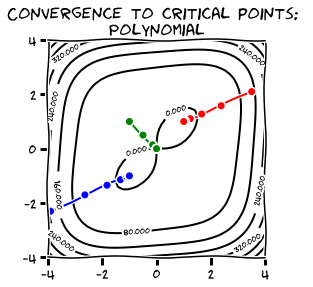
\includegraphics[width=0.45\linewidth]{convergenceNewton.png} &
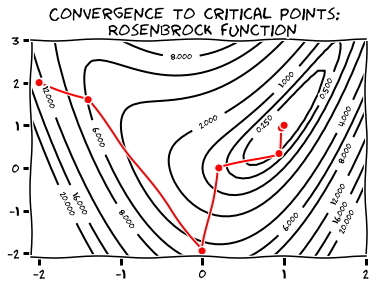
\includegraphics[width=0.55\linewidth]{convergenceNewtonRosenbrock.png} 
\end{tabular}
\caption{Newton method}
\label{figure:NewtonConvergence}
\end{figure}

\begin{remark}
Newton's Method to solve $\boldsymbol{g}=\boldsymbol{0}$, as given by the recurrence formula in equation \eqref{equation:NewtonMethod} in page \pageref{equation:NewtonMethod}, is very convenient to provide explicit descriptions of the different iterations.  However, it is hardly suitable for practical purposes, due to the computational issues involving matrix inversion.

To avoid dealing with matrix inversion, we consider the following equivalent formula:
\begin{equation}
\gradient{\boldsymbol{g}}(\x_n) \cdot \big( \x_{n+1} - \x_n \big) = -\boldsymbol{g}(\x_n)
\end{equation}
This is a simple system of linear equations, and thus much faster to solve.  

The equivalent recurrence formula to search for critical points of a twice continuously differentiable real-valued function $f \colon \field{R}^d \to \field{R}$ is thus
\begin{equation}
\Hess{f}(\x_n) \cdot (\x_{n+1}-\x_n) = -\gradient{f}(\x_n).
\end{equation}
\end{remark}

\begin{example}
The equivalent recurrence formula to the one we obtained in example \ref{example:preNewton4poly4} is as follows:
\begin{equation*}
\begin{bmatrix} 3x_n^2 & -1 \\ -1 & 3y_n^2 \end{bmatrix} \begin{bmatrix} x_{n+1}-x_n \\ y_{n+1}-y_n \end{bmatrix} = \begin{bmatrix} x_n^3 - y_n \\ y_n^3 - x_n \end{bmatrix}
\end{equation*}
All we need to do is, at each step $n$, solve for $X$ and $Y$ the system of linear equations
\begin{equation*}
\begin{cases}
3x_n^2 (X-x_n) - (Y-y_n)  = x_n^3 - y_n \\
-(X-x_n) + 3y_n^2 (Y-y_n) = y_n^2 - x_n
\end{cases}
\end{equation*}
or equivalently,
\begin{equation*}
\begin{cases}
3x_n^2 X - Y = 4x_n^3 - 2y_n \\
-X + 3y_n^2 Y = 4y_n^2 - 2x_n
\end{cases}
\end{equation*}
\end{example}

There are some theoretical results that aid in the search for a \emph{good} initial guess.  The following states a simple set of conditions on $f$ and $\x_0$ to guarantee \emph{quadratic convergence}\footnote{See Appendix \ref{appendix:convergence}} of the corresponding sequences $\{ \x_n \}_{n \in \field{N}}$ to a critical point $\xstar$.

\begin{theorem}[Quadratic Convergence Theorem]\label{theorem:QuadraticConvergence}
Suppose $f\colon \field{R}^d \to \field{R}$ is a twice continuously differentiable real-valued function, and $\xstar$ is a critical point of $f$. Let $\mathcal{N}(\x) = \x - \big[ \Hess{f}(\x) \big]^{-1} \cdot \gradient{f}(\x)$. If there exists 
\begin{enumerate}
	\item $h>0$ so that\footnote{Recall the \emph{norm} of a matrix $M$, defined by $\norm{M} = \max\{ \norm{M\cdot \x} : \norm{\x}=1 \}$.} $\big\lVert \big[ \Hess{f}(\xstar)\big]^{-1} \big\rVert \leq \tfrac{1}{h}$,
	\item $\beta>0$, $L>0$ for which $\norm{\Hess{f}(\x) - \Hess{f}(\xstar)} \leq L \norm{ \x - \xstar }$ provided $\norm{ \x - \xstar }\leq \beta$.
\end{enumerate}
In that case, for all $\x \in \field{R}^d$ satisfying $\norm{ \x - \xstar }\leq \min \{\beta, \tfrac{2h}{3L} \}$,
\begin{equation*}
\frac{\norm{ \mathcal{N}(\x) - \xstar }}{\norm{\x - \xstar}^2} \leq \frac{3L}{2h}
\end{equation*}
\end{theorem}

\begin{example}
Consider the function $f(x)=x-\log x$ on $(0,\infty)$, which has a global minimum at $x^\star=1$.  Its gradient is $f'(x)=1-\tfrac{1}{x}$, the function we studied in Example \ref{example:NewtonRaphsonChoice} in page \pageref{example:NewtonRaphsonChoice}.  We did establish then any initial guess $x_0$ should belong in the interval $(0,2)$.  We want to use Theorem \ref{theorem:QuadraticConvergence} to improve the search, so we may guarantee \emph{quadratic convergence} to the critical point.  
\begin{itemize}
	\item The Hessian is $f''(x)=x^{-2}$, and thus $\big\lVert \big[ \Hess{f}(x^\star) \big]^{-1} \big\rVert = 1$. 
	\item Notice that for all $0<x<2$,
	\begin{equation*}
	\norm{\Hess{f}(x) - \Hess{f}(x^\star)} = \big\lvert \tfrac{1}{x^2}  - 1 \big\rvert =\frac{1+x}{x^2}\abs{x-1}
	\end{equation*}
	Choosing e.g.~$\beta=\tfrac{1}{2}$, we readily obtain that $\frac{10}{9} \leq \frac{1+x}{x^2}\leq 6$;
	therefore, $\norm{\Hess{f}(x) - \Hess{f}(x^\star)} \leq 6 \abs{x-1}$, and we may choose $L=6$ for $\beta=\tfrac{1}{2}$.
\end{itemize}
Theorem \ref{theorem:QuadraticConvergence} guarantees that any initial guess $\x_0 \in \big(\tfrac{8}{9}, \tfrac{10}{9}\big)$ will give us good results.  

\begin{figure}[ht!]
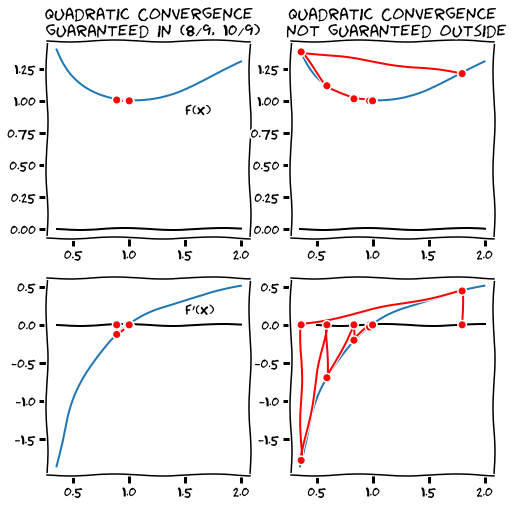
\includegraphics[width=0.75\linewidth]{quadraticConv.png}
\caption{Quadratic Convergence of the Newton-Raphson method}
\label{figure:QuadraticConvergence}
\end{figure}
\end{example}
%!TEX root = main.tex

\section{Broyden's Secant Method}
Both Newton-Raphson and Steepest descent are sound methods, with their pros and their cons.  Steepest descent always converges to a local minimum, yet slowly.  Newton has a faster convergence, but we cannot always guarantee convergence.  Another drawback of both methods is the fact that we do need expressions for both the function itself and its derivative.  The \emph{Broydent Secant method} offers an improvement to some of these issues.

\subsection{A secant method to search for roots of univariate functions}
To explain how it works, let's once again try to find an accurate value of $\sqrt{2}$ as the root of the polynomial $p(x) = x^2-2$.
\begin{enumerate}
	\item Consider two initial guesses $x_0=3$, $x_1=2.8$.  Notice $f(3)= 7 \neq 5.84 = f(2.8)$.
	\item The line that joins the points $(3, 7)$ and $( 2,8, 5.84)$ has equation
	\begin{align*}
	y - 7 &= \frac{5.84-7}{2.8-3}(x-3), \\ 
	y &= 5.8x-10.4
	\end{align*}
	and intersects the $x$--axis at
	\begin{equation*}
	x_2 = \frac{10.4}{5.8} \approx 1.7931034483
	\end{equation*}
	\item Repeat this process to get a sequence $x_n$.
\end{enumerate}
\begin{example}
Observe the result of applying this recursive process, and compare with the similar experiment we conducted using the Newton-Raphson method in page \pageref{table:Newton-Raphson}.
\begin{center}
\begin{tabular}{|r|r|r|} \hline
$n$ & $x_n$ & $f(x_n)$ \\ \hline \hline
$0$ & $3.000000000000000$ & $7.0000E+00$ \\ \hline
$1$ & $2.800000000000000$ & $5.8400E+00$ \\ \hline
$2$ & $1.793103448275862$ & $1.2152E+00$ \\ \hline
$3$ & $1.528528528528528$ & $3.3640E-01$ \\ \hline
$4$ & $1.427253172054743$ & $3.7052E-02$ \\ \hline
$5$ & $1.414717869757887$ & $1.4267E-03$ \\ \hline
$6$ & $1.414215876250105$ & $6.5446E-06$ \\ \hline
$7$ & $1.414213562785585$ & $1.1667E-09$ \\ \hline
$8$ & $1.414213562373095$ & $8.8818E-16$ \\ \hline
\end{tabular}
\end{center}
\begin{figure}[ht!]
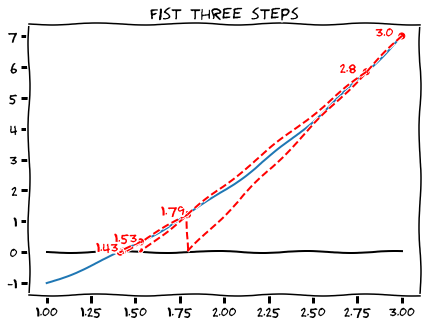
\includegraphics[width=0.6\linewidth]{images/secant.png}
\caption{Secant iterative method}\label{figure:SecantMethod}
\end{figure}
\end{example}

\begin{definition}\label{def:SecantMethod}\index{Secant method}\index{Secant method!iteration}\index{Secant method!recursive formula}
Given a function $f \colon \field{R} \to \field{R}$ and two initial guesses $x_0 \neq x_1$ satisfying $f(x_0) \neq f(x_1)$, we define the \emph{Secant method iteration} to be the sequence given by the following recursive formula
\begin{equation*}\label{equation:SecantMethod}\index{Secant method!iteration}
	x_{n+1} = x_{n-1} - \frac{x_n - x_{n-1}}{f(x_n) - f(x_{n-1})}f(x_{n-1})
\end{equation*}
The \emph{Secant method} refers to employing this sequence to search and approximate roots of the equation $f(x)=0$.
\end{definition}
%!TEX root = main.tex

\section{The Method of Steepest Descent}\index{Steepest descent}\index{Gradient!descent|see {Steepest descent}}

The method of \emph{Steepest Descent} (also known as the method of \emph{Gradient Descent}) is based upon the following property of gradients that we learned in Vector Calculus:

\begin{theorem}
If $f \colon \field{R}^d \to \field{R}$ is continuously differentiable, then at any point $\x \in \field{R}^d$, the vector $-\gradient{f}(\x)$ points in the direction of most rapid decrease for $f$ at $\x$.  The rate of decrease of $f$ at $\x$ in this direction is precisely $-\norm{\gradient{f}(\x)}$.
\end{theorem}

\begin{remark}\index{Steepest descent!direction of}\index{Direction!of steepest descent}
For this reason, the vector $-\gradient{f}(\x)/\norm{\gradient{f}(\x)}$ is called the \emph{direction of steepest descent} of $f$ at $\x$.
\end{remark}

\separator

In order to search for a local minimum for a twice continuously differentiable function $f\colon \field{R}^d \to \field{R}$, we start by choosing an initial guess $\x_0$.  
\begin{enumerate}
	\item Restrict the function $f$ over the line through $\x_0$ in the direction of $-\gradient{f}(\x_0)$:
	\begin{equation*}
	\varphi_0(t) = f\big( \x_0 - t \gradient{f}(\x_0) \big), \quad t\geq 0
	\end{equation*}
	\item \emph{Line-search}: Search for the value of $t_0 \geq 0$ that minimizes $\varphi_0$, and set\index{Line-search}
	\begin{equation*}
	\x_1 = \x_0 - t_0\gradient{f}(\x_0)
	\end{equation*}
	\item Repeat this process to get the sequence
	\begin{gather}\label{equation:SteepestDescent}
	\begin{split}
	&\x_{n+1} = \x_n - t_n \gradient{f}(\x_n), \\ &t_n = \argmin_{t\geq 0} \varphi_n(t) = \argmin_{t\geq 0} f\big(\x_n - t\gradient{f}(\x_n)\big)
	\end{split}
	\end{gather}
\end{enumerate}

\begin{remark}\index{Steepest descent!sequence of}
Sequences constructed following the formula in \eqref{equation:SteepestDescent} are said to be \emph{sequences of Steepest Descent} for $f$.

Unlike Newton-Raphson or the secant methods, this algorithm guarantees that these sequences are non-increasing: $f(\x_{n+1}) \leq f(\x_n)$ for all $n \in \field{N}$.  And even better: if there is convergence, their limit must be a critical point of $f$.  These results are formalized in Theorems \ref{theorem:SteepestDescentDescends} and \ref{theorem:SteepestDescentConvergesToCritical}  below.

Steepest descent sequences have another interesting property: on each step $n$, the direction of steepest descent is perpendicular to the direction of steepest descent of step $n+1$ (!!)  We state and prove this result in Theorem \ref{theorem:SteepestDescentPerpSteps}.
\end{remark}

\begin{theorem}\label{theorem:SteepestDescentDescends}
Let $f\colon \field{R}^d \to \field{R}$ be a continuously differentiable real-valued function, and let $\{ \x_n \}_{n\in\field{N}}$ be a sequence of steepest descent for $f$.  If $\gradient{f}(\x_N) \neq 0$, then $f(\x_{N+1}) < f(\x_N)$.
\end{theorem}

\begin{theorem}\label{theorem:SteepestDescentConvergesToCritical}
Let $f\colon \field{R}^d \to \field{R}$ be a real-valued function, let $\x_0 \in \field{R}^d$ be an initial guess.  Assume $S = \{ \x \in \field{R}^d :  f(\x) \leq f(\x_0) \}$ is a compact set and $f$ is continuously differentiable in $S$.  Under these conditions, the limit of any convergent subsequence of the associated sequence of steepest descent $\{ \x_n \}_{n\in \field{N}}$ is a critical point of $f$.
\end{theorem}

\begin{theorem}\label{theorem:SteepestDescentPerpSteps}
Let $f \colon \field{R}^d \to \field{R}$ be a continuously differentiable real-valued function, and $\{ \x_n \}_{n\in\field{N}}$ a sequence of steepest descent for $f$.  For any $n \in \field{N}$, $\langle \x_{n+2} - \x_{n+1}, \x_{n+1} - \x_n \rangle = 0$.
\end{theorem}
\begin{proof}
Consider for each $n \in \field{N}$ the function $\varphi_n(t) = f\big(\x_n -t \gradient{f}(\x_x)\big)$, with a global minimum at $t_n \geq 0$.  It must then be
\begin{equation*}
0 = \varphi_n'(t_n) = \langle \gradient{f}(\x_n), -\gradient{f}\big( \x_n - t_n \gradient{f}(\x_n)\big) \rangle = - \langle \gradient{f}(\x_{n+1}), \gradient{f}(\x_n) \rangle,
\end{equation*}
which proves that the gradient of consecutive terms of the sequence of steepest descent for $f$ are perpendicular.  Now, by virtue of the recurrence formula \eqref{equation:SteepestDescent},
\begin{align*}
\langle \x_{n+2} - \x_{n+1}, &\,\x_{n+1} - \x_n \rangle = \langle t_{n+1}\gradient{f}(\x_{n+1}), t_n \gradient{f}(\x_n) \rangle \\
&= t_{n+1}t_n \langle \gradient{f}(\x_{n+1}), \gradient{f}(\x_n) \rangle = 0, 
\end{align*}
which proves the statement.
\end{proof}

\begin{example}
For the polynomial function $p_4(x,y) = x^4-4xy+y^4$ from Example \ref{example:NewtonPoly4}, using the same initial guesses as in Example \ref{example:preNewton4poly4}, we find the following behavior:
\begin{itemize}
	\item Starting at $(x_0, y_0) = (-1.0,1.0)$, the sequence jumps to $(0,0)$ in one step.  At that point, since the gradient of the function is zero, the method of Steepest descent ceases to work.
	% \begin{table}[ht!]
	\begin{center}
	\begin{tabular}{|r|r|r|r|} \hline 
	$n$ & $x_n$ & $y_n$ & $f(x_n,y_n)$ \\ \hline \hline 
	$0$ & $-1.000000$ & $1.000000$ & $6.000000$ \\ \hline 
	$1$ & $0.000000$ & $0.000000$ & $0.000000$ \\ \hline 
	$2$ & \texttt{nan} & \texttt{nan} & \texttt{nan} \\ \hline 
	\end{tabular}
	% \caption{Steepest Descent: Convergence to $(0,0)$ accurately in exactly one step.}
	% \label{table:SD00}
	% \end{table}
	\end{center}
	\item Starting at $(x_0,y_0) = (3.5, 2.1)$, the sequence converges to $(1,1)$.
	% \begin{table}[ht!]
	\begin{center}
	\begin{tabular}{|r|r|r|r|} \hline 
	$n$ & $x_n$ & $y_n$ & $f(x_n,y_n)$ \\ \hline \hline 
	$0$ & $3.500000$ & $2.100000$ & $140.110600$ \\ \hline 
	$1$ & $1.044472$ & $1.753064$ & $3.310777$ \\ \hline 
	$2$ & $1.141931$ & $1.063276$ & $-1.878163$ \\ \hline 
	$3$ & $1.008581$ & $1.044435$ & $-1.988879$ \\ \hline 
	$4$ & $1.013966$ & $1.006319$ & $-1.998931$ \\ \hline 
	$5$ & $1.000898$ & $1.004472$ & $-1.999891$ \\ \hline 
	$6$ & $1.001437$ & $1.000651$ & $-1.999989$ \\ \hline 
	$7$ & $1.000093$ & $1.000461$ & $-1.999999$ \\ \hline 
	% \end{tabular}~\begin{tabular}{|r|r|r|r|} \hline 
	% $n$ & $x_n$ & $y_n$ & $f(x_n,y_n)$ \\ \hline \hline 
	$8$ & $1.000149$ & $1.000067$ & $-2.000000$ \\ \hline 
	$9$ & $1.000010$ & $1.000048$ & $-2.000000$ \\ \hline 
	$10$ & $1.000015$ & $1.000007$ & $-2.000000$ \\ \hline 
	$11$ & $1.000001$ & $1.000005$ & $-2.000000$ \\ \hline 
	$12$ & $1.000002$ & $1.000001$ & $-2.000000$ \\ \hline 
	$13$ & $1.000000$ & $1.000001$ & $-2.000000$ \\ \hline 
	$14$ & $1.000000$ & $1.000000$ & $-2.000000$ \\ \hline 
	$15$ & $1.000000$ & $1.000000$ & $-2.000000$ \\ \hline 
	\end{tabular}
	% \caption{Steepest Descent: Convergence to $(1,1)$ with 6-digit accuracy in 13 steps.}
	% \label{table:SD11}
	% \end{table}
	\end{center}
	\item Starting at $(x_0, y_0) = (-13.5, -7.3)$, the sequence converges to $(1,1)$ as well.
	% \begin{table}[ht!]
	\begin{center}
	\begin{tabular}{|r|r|r|r|} \hline 
	$n$ & $x_n$ & $y_n$ & $f(x_n,y_n)$ \\ \hline \hline 
	$0$ & $-13.500000$ & $-7.300000$ & $35660.686600$ \\ \hline 
	$1$ & $2.362722$ & $-4.871733$ & $640.498302$ \\ \hline 
	$2$ & $1.434154$ & $1.194162$ & $-0.586492$ \\ \hline 
	$3$ & $1.021502$ & $1.130993$ & $-1.896212$ \\ \hline 
	$4$ & $1.038817$ & $1.017881$ & $-1.991558$ \\ \hline 
	$5$ & $1.002305$ & $1.012291$ & $-1.999167$ \\ \hline 
	$6$ & $1.003909$ & $1.001808$ & $-1.999917$ \\ \hline 
	$7$ & $1.000236$ & $1.001246$ & $-1.999992$ \\ \hline 
	% \end{tabular}~\begin{tabular}{|r|r|r|r|} \hline 
	% $n$ & $x_n$ & $y_n$ & $f(x_n,y_n)$ \\ \hline \hline 
	$8$ & $1.000399$ & $1.000185$ & $-1.999999$ \\ \hline 
	$9$ & $1.000024$ & $1.000127$ & $-2.000000$ \\ \hline 
	$10$ & $1.000041$ & $1.000019$ & $-2.000000$ \\ \hline 
	$11$ & $1.000002$ & $1.000013$ & $-2.000000$ \\ \hline 
	$12$ & $1.000004$ & $1.000002$ & $-2.000000$ \\ \hline 
	$13$ & $1.000000$ & $1.000001$ & $-2.000000$ \\ \hline 
	$14$ & $1.000000$ & $1.000000$ & $-2.000000$ \\ \hline 
	$15$ & $1.000000$ & $1.000000$ & $-2.000000$ \\ \hline 
	\end{tabular}
	% \caption{Steepest Descent: Convergence to $(1,1)$ with 6-digit accuracy in 14 steps.}
	% \label{table:SD-1-1}
	% \end{table}
	\end{center}
\end{itemize}
\begin{figure}[ht!]
% \begin{tabular}{c}
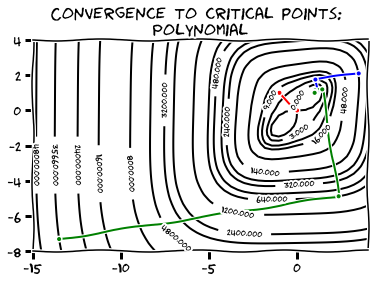
\includegraphics[width=0.7\linewidth]{images/convergenceSteepest.png}
% 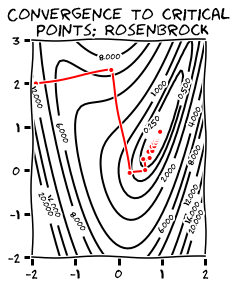
\includegraphics[width=0.65\linewidth]{images/SDR3.png}
% \end{tabular}
\caption{The Method of Steepest Descent: Polynomial function}
\label{figure:SteepestConvergenceP}
\end{figure}
\end{example}

\begin{example}\label{example:SDR}\index{Function!Rosenbrock}
Notice what happens when we try to implement the same process on the Rosenbrock function $\mathcal{R}_{1,1}(x,y) = (1-x)^2 + (y-x^2)^2$, with the initial guess $(x_0, y_0) = (-2,2)$.  The sequence does converge to the minimum $(1,1)$, albeit very slowly.
\begin{center}
\begin{tabular}{|r|r|r|r|} \hline 
 $n$ & $x_n$ & $y_n$ & $f(x_n,y_n)$ \\ \hline \hline 
$0$ & $-2.000000$ & $2.000000$ & $13.000000$ \\ \hline 
$1$ & $-0.166290$ & $2.309522$ & $6.567163$ \\ \hline 
$2$ & $0.256054$ & $-0.056128$ & $0.568264$ \\ \hline 
$3$ & $0.613477$ & $0.007683$ & $0.285318$ \\ \hline 
$4$ & $0.568566$ & $0.259241$ & $0.190235$ \\ \hline 
$5$ & $0.715784$ & $0.285524$ & $0.132227$ \\ \hline 
$6$ & $0.689755$ & $0.431319$ & $0.098227$ \\ \hline 
$7$ & $0.779264$ & $0.447299$ & $0.074310$ \\ \hline 
$8$ & $0.761554$ & $0.546496$ & $0.057977$ \\ \hline 
$9$ & $0.823325$ & $0.557524$ & $0.045696$ \\ \hline 
$10$ & $0.810322$ & $0.630358$ & $0.036667$ \\ \hline 
$11$ & $0.855862$ & $0.638488$ & $0.029614$ \\ \hline 
$12$ & $0.845883$ & $0.694385$ & $0.024199$ \\ \hline 
$13$ & $0.880846$ & $0.700627$ & $0.019862$ \\ \hline 
$14$ & $0.872964$ & $0.744776$ & $0.016437$ \\ \hline 
$15$ & $0.900551$ & $0.749702$ & $0.013647$ \\ \hline 
$16$ & $0.894200$ & $0.785276$ & $0.011399$ \\ \hline 
\end{tabular}~\begin{tabular}{|r|r|r|r|} \hline
 $n$ & $x_n$ & $y_n$ & $f(x_n,y_n)$ \\ \hline \hline 
$17$ & $0.916394$ & $0.789239$ & $0.009544$ \\ \hline 
$18$ & $0.911201$ & $0.818326$ & $0.008028$ \\ \hline 
$19$ & $0.929317$ & $0.821560$ & $0.006766$ \\ \hline 
$20$ & $0.925024$ & $0.845608$ & $0.005723$ \\ \hline 
$21$ & $0.939976$ & $0.848277$ & $0.004847$ \\ \hline 
$22$ & $0.936397$ & $0.868329$ & $0.004118$ \\ \hline 
$23$ & $0.948845$ & $0.870551$ & $0.003502$ \\ \hline 
$24$ & $0.945840$ & $0.887385$ & $0.002986$ \\ \hline 
$25$ & $0.956276$ & $0.889248$ & $0.002548$ \\ \hline 
$26$ & $0.953739$ & $0.903457$ & $0.002178$ \\ \hline 
$27$ & $0.962537$ & $0.905028$ & $0.001864$ \\ \hline 
$28$ & $0.960386$ & $0.917075$ & $0.001597$ \\ \hline 
$29$ & $0.967837$ & $0.918405$ & $0.001369$ \\ \hline 
$30$ & $0.966007$ & $0.928657$ & $0.001176$ \\ \hline 
$31$ & $0.972342$ & $0.929788$ & $0.001010$ \\ \hline 
$32$ & $0.970780$ & $0.938539$ & $0.000869$ \\ \hline 
$33$ & $0.976182$ & $0.939503$ & $0.000748$ \\ \hline 
\end{tabular}
\end{center}
\end{example}

\begin{figure}[ht!]
% \begin{tabular}{c}
% 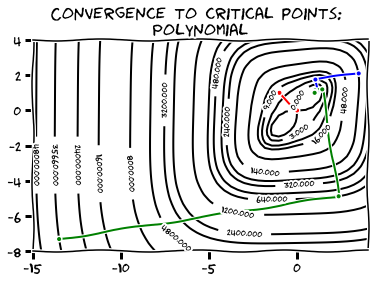
\includegraphics[width=0.65\linewidth]{images/convergenceSteepest.png} \\
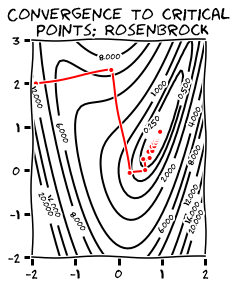
\includegraphics[width=0.6\linewidth]{images/SDR3.png}
% \end{tabular}
\caption{The Method of Steepest Descent: Rosenbrock Function}
\label{figure:SteepestConvergenceR}
\end{figure}

\subsection{Efficiency of Steepest Descent Method}

The analysis of efficiency of the method of Steepest descent is quite involved, but it boils down to studying the efficiency of Steepest descent for quadratic functions---since any function can be approximated using a Taylor's polynomial of degree two.  We will study that easier case in these notes.

\begin{theorem}[Taylor's Formula]\index{Theorem!Taylor's formula}
If $f\colon \field{R}^d \to \field{R}$ is a real-valued function of $d$ variables with continuous first and second partial derivatives on $\field{R}^d$, then for any choice $\x, \y \in \field{R}^d$, there exists a point $\boldsymbol{\xi} = \boldsymbol{\xi}(\x, \y)$ in the segment joining $\x$ and $\y$ so that
\begin{equation*}
f(\x) = f(\y) + \langle \gradient{f}(\y), \x - \y \rangle + \tfrac{1}{2} \quadratic{\Hess{f}(\boldsymbol{\xi})}(\x - \y)
\end{equation*}
\end{theorem}

\separator

Assume we have a quadratic function $p\colon \field{R}^d \to \field{R}$ satisfying $p(\boldsymbol{0}) = 0$.  There exist a $d$-dimensional vector $D = \big[q_1, \dotsc, q_d\big]$ and a symmetric matrix $Q = \big[ q_{jk} \big]_{j,k=1}^d$ (with $q_{jk}=q_{kj}$ for all $1\leq j,k \leq d$) so that
\begin{equation*}
p(\x) = \langle D, \x \rangle + \tfrac{1}{2}\quadratic{Q}(\x) = \sum_{k=1}^d \big( \tfrac{1}{2}q_{kk}x_k^2 + q_k x_k\big) + \sum_{1\leq j<k \leq d} q_{jk} x_j x_k
\end{equation*}
The gradient of this function is thus $\gradient{p}(\x) = x \cdot Q + D$.  It has one unique critical point $\xstar = -D Q^{-1}$ (Why?).  At that point, it is 
\begin{align}
p(\xstar) &= \tfrac{1}{2} \big( -D Q^{-1} \big)  Q \transpose{\big( -D Q^{-1} \big)} + D \transpose{\big( -D Q^{-1} \big)} \nonumber \\ 
&= \tfrac{1}{2} D Q^{-1} \transpose{D} - D Q^{-1} \transpose{D} \nonumber \\
&= -\tfrac{1}{2} D Q^{-1} \transpose{D} = -\tfrac{1}{2}\quadratic{(Q^{-1})}(D). \label{equation:pstarSD}
\end{align}
If $\x_n$ is a term in a sequence of steepest descent, then to compute $\x_{n+1}$ we proceed as follows:
\begin{enumerate}
	\item The direction of steepest descent at $\x_n$ is 
	\begin{equation*}\v_n = -\gradient{p}(\x_n) = -(x_n Q + D).
	\end{equation*}
	\item The restriction $\varphi\colon (0,\infty) \to \field{R}$ of the quadratic function $p$ over the half-line through $\x_n$ in the direction $\v_n$ is given by
	\begin{align*}
	\varphi(t) &= p( \x_n + t \v_n ) \\
	&= \tfrac{1}{2}(\x_n + t\v_n ) Q \transpose{(\x_n + t\v_n )} + D\transpose{(\x_n + t\v_n )} \\
	&= \tfrac{1}{2} \x_n Q \transpose{(\x_n + t\v_n )} + \tfrac{1}{2}t\v_n Q \transpose{(\x_n + t\v_n )} \\
	&\quad+D \transpose{\x}_n + tD \transpose{\v}_n \\
	&= \tfrac{1}{2}\x_n Q \transpose{\x}_n + \tfrac{1}{2} t\x_n Q \transpose{\v}_n + \tfrac{1}{2} t \v_n Q \transpose{\x}_n + \tfrac{1}{2} t^2 \v_n Q \transpose{\v}_n \\
	&\quad + D \transpose{\x}_n + t D \transpose{\v}_n \\
	&= \tfrac{1}{2} \underbrace{\v_n Q \transpose{\v}_n}_{\quadratic{Q}(\v_n)} t^2 + \underbrace{\tfrac{1}{2}\x_n Q \transpose{\x}_n + D \transpose{\x}_n}_{p(\x_n)} + tD\transpose{\v}_n + t \x_n Q \transpose{\v}_n \\
	&= \tfrac{1}{2} \quadratic{Q}(\v_n) t^2  + p(\x_n) + t \underbrace{\big( x_n Q + D \big)}_{-\v_n} \transpose{\v}_n \\
	&= \tfrac{1}{2}t^2 \v_n Q \transpose{\v}_n -  t \v_n \transpose{\v}_n + p(\x_n) \\
	&= \tfrac{1}{2} \quadratic{Q}(\v_n)t^2 - \norm{\v_n}^2 t + p(\x_n)
	\end{align*}
	\item The restriction function has its global minimum at
	\begin{equation*}
	t_n = \frac{\norm{\v_n}^2}{\quadratic{Q}(\v_n)};
	\end{equation*}
	therefore, the next iteration occurs at
	\begin{equation*}
	x_{n+1} = x_n + t_n \v_n = x_n + \frac{\norm{\v_n}^2}{\quadratic{Q}(\v_n)} \v_n 
	\end{equation*}
\end{enumerate}

\separator

We want to observe the convergence behavior of the sequence of evaluations $\{ p(\x_n) \}_{n \in \field{N}}$ to $p(\xstar)$.  We have
\begin{align*}
p(\x_{n+1}) &= p(\x_n + \tfrac{\norm{\v_n}^2}{\quadratic{Q}(\v_n)} \v_n) \\
&= \tfrac{1}{2} \quadratic{Q}(\v_n) \big( \tfrac{\norm{\v_n}^2}{\quadratic{Q}(\v_n)} \big)^2 - \norm{\v_n}^2 \tfrac{\norm{\v_n}^2}{\quadratic{Q}(\v_n)} + p(\x_n) \\
&= p(\x_n) - \frac{\norm{\v_n}^4}{2\quadratic{Q}(\v_n)}; 
\intertext{therefore,}
\frac{p(\x_{n+1}) - p(\xstar)}{p(\x_n)- p(\xstar)} &= \frac{p(\x_n) - p(\xstar) - \frac{\norm{\v_n}^4}{2\quadratic{Q}(\v_n)}}{p(\x_n) - p(\xstar)} \\
&= 1 - \frac{\norm{\v_n}^4}{ 2\quadratic{Q}(\v_n) \big( p(\x_n) - p(\xstar) \big)} \\
&= 1 - \frac{\norm{\v_n}^4}{2\quadratic{Q}(\v_n) \big( \tfrac{1}{2}\x_n Q \transpose{\x}_n + D \transpose{\x}_n + \tfrac{1}{2} DQ^{-1}\transpose{D} \big)} \\
&= 1 - \frac{\norm{\v_n}^4}{ \quadratic{Q}(\v_n) \big( \x_n Q \transpose{\x}_n+ 2D\transpose{\x}_n + DQ^{-1}\transpose{D} \big) }.
\end{align*}
Note in the denominator we may rewrite some of the terms:
\begin{align*}
\x_n Q \transpose{\x}_n &= \x_n Q (Q^{-1}Q) \transpose{\x}_n = (\x_n Q) Q^{-1} \transpose{(\x_n Q)}, \\
2D \transpose{\x}_n &= D\transpose{\x}_n + D\transpose{\x}_n = \x_n \transpose{D} + D (Q^{-1}Q) \transpose{\x}_n \\
&= \x_n (QQ^{-1}) \transpose{D} + D Q^{-1} \transpose{(\x_n Q)} \\
&= (\x_n Q) Q^{-1} \transpose{D} + D Q^{-1} \transpose{(\x_n Q)}.
\end{align*} 
This allows us to rewrite in the following convenient form 
\begin{align*}
\frac{p(\x_{n+1}) - p(\xstar)}{p(\x_n)- p(\xstar)} &= 1 - \frac{\norm{\v_n}^4}{ \quadratic{Q}(\v_n) (\x_n Q + D) Q^{-1} \transpose{(\x_nQ + D)} } \\
&= 1 - \frac{\norm{\v_n}^4}{\quadratic{Q}(\v_n) \quadratic{(Q^{-1})}(\v_n)}.
\end{align*}

We are ready to state the main result of this subsection:
\begin{theorem}\label{theorem:KantorovichEstimate}\index{Steepest descent!error}
Given a $d$-dimensional vector $D$, and a positive definite symmetric matrix $Q$ of size $d \times d$, consider the quadratic function $p(\x) = \tfrac{1}{2}\quadratic{Q}(\x) + \langle D , \x \rangle$.  Any sequence $\{ \x_n \}_{n \in \field{N}}$ of steepest descent converges to the global minimum $\xstar = -DQ^{-1}$.  The sequence of evaluations $\{ p(\x_n) \}_{n \in \field{N}}$ converges linearly to $p(\xstar) = -\tfrac{1}{2}\quadratic{(Q^{-1})}(D)$.  In particular, if $0 < \lambda_1 \leq \lambda_2 \leq \dotsb \leq \lambda_d$ are the eigenvalues of $Q$, then 
\begin{equation*}
\frac{p(\x_{n+1}) - p(\xstar)}{p(\x_n)- p(\xstar)} \leq \bigg( \frac{\lambda_d -\lambda_1}{\lambda_d + \lambda_1} \bigg)^2
\end{equation*}
\end{theorem}
\begin{proof}
We start by offering the following lower bound estimate\footnote{This is left as and advanced exercise. It is not too tricky; if you are stuck, see e.g.~\cite[section 1.3.1]{bertsekas1999nonlinear} for a proof.} involving the associated directions of steepest descent $\v_n$ in terms of the largest and smallest eigenvalues of $Q$.  For all $n \in \field{N}$,
\begin{equation}\label{equation:KantorovichEstimate}\index{Theorem!Kantorovich estimate}
\frac{\norm{\v_n}^4}{\quadratic{Q}(\v_n) \quadratic{(Q^{-1})}(\v_n)} \geq \frac{4\lambda_0\lambda_d}{(\lambda_0 + \lambda_d)^2}
\end{equation}
We have then
\begin{align*}
\frac{p(\x_{n+1}) - p(\xstar)}{p(\x_n)- p(\xstar)} &= 1 - \frac{\norm{\v_n}^4}{ \quadratic{Q}(\v_n) \quadratic{(Q^{-1})}(\v_n) } \\
&\leq 1 - \frac{4\lambda_1 \lambda_d}{(\lambda_1 + \lambda_d)^2} = \bigg( \frac{\lambda_d - \lambda_1}{\lambda_d + \lambda_1} \bigg)^2 \qedhere
\end{align*}
\end{proof}

\begin{example}\label{example:SDconvergenceRate}
The global minimum value of the quadratic function $p(x,y) = 5x^2 + 5y^2 -xy -11x +11y +11$ is zero, and found at $(1,-1)$.  Notice that we may write this function in the form $p(x,y) = \tfrac{1}{2}\quadratic{Q}(x,y) + \langle D, [x,y] \rangle + 11$, where
\begin{equation*}
D = [ -11, 11], \qquad Q = \begin{bmatrix} 10 & -1 \\ 10 & -1 \end{bmatrix}.
\end{equation*}
The symmetric matrix $Q$ has eigenvalues $\lambda_1 = 9 >0$, $\lambda_2 = 11 > 0$ and is therefore positive definite.  Theorem \ref{theorem:KantorovichEstimate} states that sequences of steepest descent exhibit linear convergence with a rate of convergence not larger than $\delta = \big( \tfrac{11-9}{11+9} \big)^2 = 0.01$.

Observe the computations of the first six iterations for values of the ratios $\frac{p(\x_n)}{p(\x_{n-1})}$ when we use $(1.5,3.5)$ as our initial guess.
\begin{center}
\begin{tabular}{|r|r|r|r|r|} \hline 
 $n$ & $x_n$ & $y_n$ & $p(x_n,y_n)$ & $\boldsymbol{\frac{p(x_n,y_n)}{p(x_{n-1},y_{n-1})}}$ \\ \hline \hline 
$0$ & $1.5000000000$ & $3.5000000000$ & $100.2500000000$ &  \\ \hline 
$1$ & $1.4498874016$ & $-0.9600212545$ & $1.0019989373$ & $\boldsymbol{0.0099950019}$ \\ \hline 
$2$ & $1.0049975009$ & $-0.9550224916$ & $0.0100149812$ & $\boldsymbol{0.0099950019}$ \\ \hline 
$3$ & $1.0044966254$ & $-0.9996004124$ & $0.0001000998$ & $\boldsymbol{0.0099950019}$ \\ \hline 
$4$ & $1.0000499500$ & $-0.9995504497$ & $0.0000010005$ & $\boldsymbol{0.0099950019}$ \\ \hline 
$5$ & $1.0000449438$ & $-0.9999960061$ & $0.0000000100$ & $\boldsymbol{0.0099950042}$ \\ \hline 
$6$ & $1.0000004993$ & $-0.9999955067$ & $0.0000000001$ & $\boldsymbol{0.0099950528}$ \\ \hline 
\end{tabular}
\end{center}
\end{example}

%!TEX root = main.tex

\section{Effective Algorithms for Unconstrained Optimization}
All of the methods we have explored so far (Newton-Raphson, Secant methods, Steepest descent) offer sound algorithms to compute local extrema of real-valued functions $f \colon \field{R}^d \to \field{R}$. The do have some pros and cons.  
\begin{itemize}
	\item The method of Steepest descent always converges to a local minimum, yet slowly.  In order to obtain new approximations, we have to solve many different one-dimensional optimizations, each of them offering their own computational issues. 
	\item Both Newton-Raphson and Secant methods offers faster sequences, but we cannot always guarantee convergence.  
	\item Another drawback of both Newton-Raphson and Steepest descent is the fact that we do need expressions for function itself, its gradient and Hessian matrix.  
\end{itemize}

%!TEX root = notes.tex

\section{Exercises}

\begin{problem}
Consider the function 
\begin{equation*}
f(x) = 9x -4\log(x-7)
\end{equation*}
\begin{enumerate}
	\item Find the domain $D$ of $f$.
	\item Compute an exact formula for the Newton-Raphson iterate $x_{n+1}$ for an initial guess $x_0 \in D$.
	\item Compute five iterations of the Newton-Raphson method starting at each of the following initial guesses:
	\begin{enumerate}
		\item $x_0 = 7.4$.
		\item $x_0 = 7.2$.
		\item $x_0 = 7.01$.
		\item $x_0 = 7.8$.
		\item $x_0 = 7.88$.
	\end{enumerate}
	\item Prove that the Newton-Raphson method converges to the optimal solution for all initial guesses $x_0 \in (7,7.8888)$.
	\item What is the behavior of the Newton-Raphson method if the initial guess is not in the interval $(7,7.8888)$?
\end{enumerate}
\end{problem}

\begin{problem}
Consider the function 
\begin{equation*}
f(x) = 6x -4\log(x-2) -3\log(25-x)
\end{equation*}
\begin{enumerate}
	\item Find the domain $D$ of $f$.
	\item Compute an exact formula for the Newton-Raphson iterate $x_{n+1}$ for an initial guess $x_0 \in D$.
	\item Compute five iterations of the Newton-Raphson method starting at each of the following initial guesses:
	\begin{enumerate}
		\item $x_0 = 2.6$.
		\item $x_0 = 2.7$.
		\item $x_0 = 2.4$.
		\item $x_0 = 2.8$.
		\item $x_0 = 3$.
	\end{enumerate}
	\item Prove that the Newton-Raphson method converges to the optimal solution for all initial guesses $x_0 \in (2,3.05)$.
	\item What is the behavior of the Newton-Raphson method if the initial guess is not in the interval $(2,3.05)$?
\end{enumerate}
\end{problem}

%%%%% chapter 4
\chapter[Constrained Optimization]{Existence and Characterization of Extrema for Constrained Optimization}
\label{chapter:ConstrainedExistenceCharacterization}
%!TEX root = main.tex

\chapter[Constrained Optimization]{Existence and Characterization of Extrema for Constrained Optimization}
\label{chapter:ConstrainedExistenceCharacterization}
%!TEX root = main.tex

\section{Necessary Conditions}
We begin with two results that focus on the structure of the equality constraints.
\begin{theorem}[Geometric Necessary Condition for Linear Equality Constraints]\index{Theorem!Geometric necessary condition}
If $(P)$ is a consistent program with linear equality constraints $h_k(\x) = \langle \boldsymbol{a}_k, \x \rangle + b_k$ ($\boldsymbol{a}_k \in \field{R}^d$, $b_k \in \field{R}$) for all $1 \leq k \leq \ell$, then for all feasible local minima $\x \in S$,
\begin{equation*}
\mathcal{F}_0(\x) \cap \mathcal{G}_0(\x) \cap \mathcal{H}_0(\x) = \emptyset.
\end{equation*}
\end{theorem}

\begin{theorem}[Geometric Necessary Condition for Linearly Independent Equality Constraints]\index{Theorem!Geometric necessary condition}
If $\x \in S$ is a feasible local minimum for the consistent program $(P)$, and the gradient vectors $\{ \gradient{h_k}(\x) : 1 \leq k \leq \ell \}$ are linearly independent, then $\mathcal{F}_0(\x) \cap \mathcal{G}_0(\x) \cap \mathcal{H}_0(\x) = \emptyset$.
\end{theorem}

\separator

As a consequence, an algebraic version of this geometric necessary condition gives the following result.

\begin{theorem}[Fritz John Necessary Conditions]\index{Theorem!Fritz John necessary conditions}
If $\x \in S$ is a feasible local minimum of the consistent program $(P)$, then there exist $u_k \geq 0$ for $0\leq k \leq m$, and $v_1, \dots, v_\ell \in \field{R}$ so that
\begin{enumerate}
 	\item $[u_0, u_1, \dotsc, u_m, v_1 \dotsc, v_\ell ] \neq \boldsymbol{0}$,
 	\item $u_k g_k(\x) = 0$ for all $1 \leq k \leq m$.
 	\item $u_0 \gradient{f}(\x) + \sum_{k=1}^m u_k \gradient{g_k}(\x) + \sum_{k=1}^\ell v_k \gradient{h_k}(\x) = 0$.
 \end{enumerate}
\end{theorem}

\begin{theorem}[Karush-Kuhn-Tucker Necessary Conditions]\index{Theorem!Karush-Kuhn-Tucker}\index{Theorem!KKT necessary conditions}\label{theorem:KKTnecessary}
If $\x \in S$ is a feasible local minimum of the consistent program $(P)$ for which all the vectors $\{ \gradient{h_k}(\x), \gradient{g_j}(\x) : 1 \leq k \leq \ell, j \in \mathcal{I}(\x) \}$ are linearly independent, then there exist $u_k \geq 0$ for $1\leq k \leq m$, and $v_1, \dots, v_\ell \in \field{R}$ so that
\begin{enumerate}
 	\item\label{item:KKTnecessary1} $[u_1, \dotsc, u_m, v_1 \dotsc, v_\ell ] \neq \boldsymbol{0}$,
 	\item\label{item:KKTnecessary2} $u_k g_k(\x) = 0$ for all $1 \leq k \leq m$.
 	\item\label{item:KKTnecessary3} $\gradient{f}(\x) + \sum_{k=1}^m u_k \gradient{g_k}(\x) + \sum_{k=1}^\ell v_k \gradient{h_k}(\x) = 0$.
 \end{enumerate}
\end{theorem}

\begin{remark}\index{KKT conditions}
The conditions \ref{item:KKTnecessary1}, \ref{item:KKTnecessary2} and \ref{item:KKTnecessary3} of Theorem \ref{theorem:KKTnecessary} are called \emph{the KKT conditions} of the program $(P)$ in the literature.
\end{remark}

\begin{example}
Continuing with example \ref{example:feasibleP1}, let's check if the point $(0,0)$ is a candidate to optimal solution of this program.  Let's use Theorem \ref{theorem:KKTnecessary} to verify this claim:
\begin{align*}
\gradient{f}(x,y) &= [ 4x^3, 4y^3 ] &\gradient{f}(0,0) &= [0,0], \\
\gradient{g_1}(x,y) &= [ 2x, 0 ] &\gradient{g_1}(0,0) &= [0,0], \\
\gradient{g_2}(x,y) &= [0, 2y] &\gradient{g_2}(0,0) &= [0,0], \\
\gradient{g_3}(x,y) &= \big[e^{x+y}, e^{x+y} \big] &\gradient{g_3}(0,0) &= [1,1].
\end{align*}
Notice how the gradients \emph{line up} nicely---can we find $u_k \geq 0$ (not all of them simultaneously equal to zero) so that the following linear combination is equal to $[0,0]$?
\begin{gather*}
\gradient{f}(0,0) + u_1 \gradient{g_1}(0,0) + u_2 \gradient{g_2}(0,0) + u_3 \gradient{g_3}(0,0) = [0,0], \\
[0,0] + u_1[0,0] + u_2[0,0] +u_3[1,1] = [0,0],
\end{gather*}
We may select, for instance $u_1=u_2=1$, $u_3=0$, which proves that the point $(0,0)$ is indeed a candidate for optimal solution of $(P)$.
\end{example}

\begin{example}\label{example:feasibleP3}
Set $f(x,y)=(x-12)^2+(y+6)^2$.  Consider the program $(P)$ designed to find the global minimum of this function on the set $S=\{ (x,y) \in \field{R}^2 : x^2+3x+y^2-4.5y \leq 6.5, (x-9)^2 +y^2 \leq 64, 8x+4y=20 \}$.  We want to prove that the point $(2,1)$ is a good candidate for optimal solution of $(P)$.
The point $(2,1)$ is feasible.  To see this, set 
\begin{align*}
g_1(x,y) &=x^2+3x+y^2-4.5y-6.5, \\
g_2(x,y) &=(x-9)^2+y^2-64, \\
h_1(x,y) &=8x+4y-20,
\end{align*}
(or simpler equivalent constraints), and notice that
\begin{equation*}
g_1(2,1)=-12, \quad g_2(2,1)=-14, \quad h_1(2,1)=0.
\end{equation*}
\begin{figure}[ht!]
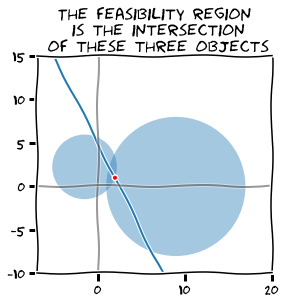
\includegraphics[width=0.5\linewidth]{images/feasibleP3.png}
\caption{Feasibility region for $(P)$ in example \ref{example:feasibleP3}}
\label{figure:feasibleP3}
\end{figure}
We have concluded that $(P)$ is consistent.  To verify that $(2,1)$ is candidate for optimal solution of $(P)$, we may now use Theorem \ref{theorem:KKTnecessary} and check if the gradients line up nicely for this point:
\begin{align*}
\gradient{f}(x,y)   &= [ 2(x-12), 2(y+6) ] &\gradient{f}(2,1)   &= [-20, 14], \\
\gradient{g_1}(x,y) &= [ 2x+3, 2y-4.5 ]    &\gradient{g_1}(2,1) &= [  7, -2.5], \\
\gradient{g_2}(x,y) &= [ 2(x-9), 2y ]      &\gradient{g_2}(2,1) &= [-14, 2], \\
\gradient{h_1}(x,y) &= [ 8, 4]             &\gradient{h_1}(2,1) &= [  8, 4], 
\end{align*}
Looking for $u_k \geq 0, v_1 \in \field{R}$ (not all of them simultaneously equal to zero) so that the following linear combination is equal to $[0,0]$.
\begin{align*}
\gradient{f}(2,1) + u_1 \gradient{g_1}(2,1) + u_2 \gradient{g_2}(2,1) + v_1 \gradient{h_1}(2,1) &= [0,0], \\
[-20,14] + u_1 [7,-2.5] + u_2 [-14,2] + v_1 [8,4] = [0,0]
\end{align*}
or equivalently
\begin{equation*}
\begin{bmatrix} 7 & -14 \\ -2.5 & 2 \end{bmatrix} \begin{bmatrix} u_1 \\ u_2 \end{bmatrix} = \begin{bmatrix} 20 - 8v_1 \\ -14-4v_1 \end{bmatrix}
\end{equation*}
Among all possible solutions, pick for instance $u_1=4$, $u_2=0$ and $v_1=-1$ to prove that the point $(2,1)$ is indeed a good candidate for the optimal solution of $(P)$.
\end{example}

\separator

Let's examine a different situation.

\begin{theorem}[Slater Necessary Condition]\label{theorem:Slater}\index{Theorem!Slater condition}
Suppose that the inequality constraints $g_k$ of a super-consistent program $(P)$ are pseudo-convex ($1\leq k \leq m$), the equality constraints $h_k$ are linear ($1\leq k \leq \ell$), and the vectors $\gradient{h_k}$ are linearly independent, then the KKT conditions \ref{item:KKTnecessary1}, \ref{item:KKTnecessary2} and \ref{item:KKTnecessary3} of Theorem \ref{theorem:KKTnecessary} are necessary to characterize optimal solutions of $(P)$.
\end{theorem}

\begin{theorem}
If all constraints of a consistent program $(P)$ are linear, then the KKT conditions \ref{item:KKTnecessary1}, \ref{item:KKTnecessary2} and \ref{item:KKTnecessary3} of Theorem \ref{theorem:KKTnecessary} are necessary to characterize optimal solutions of $(P)$.
\end{theorem}
%!TEX root = main.tex

\section{Sufficient Conditions}

It all boils down to a single result.

\begin{theorem}[KKT Sufficient Conditions]\label{theorem:KKTsufficient}\index{Theorem!KKT sufficient conditions}\index{Theorem!Karush-Kuhn-Tucker}
Let $\x \in S$ be a feasible point of the consistent program $(P)$ for which there are multipliers $\lambda_k \geq 0$ ($1\leq k \leq m)$ and $\mu_k \in \field{R}$ ($1\leq k \leq \ell$) satisfying the conditions \ref{item:KKTnecessary1} and \ref{item:KKTnecessary2} of Theorem \ref{theorem:KKTnecessary}. If $f$ is pseudo-convex, $g_k$ is quasi-convex for all $1\leq k \leq m$, and $h_k$ is linear for all $1\leq k \leq \ell$, then $\x$ is a global optimal solution of $(P)$.
\end{theorem}

\begin{example}
We saw that the point $(0,0)$ satisfies the KKT conditions for the super-consistent convex program $(P)$ in Example \ref{example:feasibleP1}.  As a consequence of Theorems \ref{theorem:FritzJohn} and \ref{theorem:KKTsufficient}, this point must be the optimal global minimum of $(P)$.

We also saw that the point $(2,1)$ satisfies the KKT conditions for the program $(P)$ in Example \ref{example:feasibleP3}.  It is not hard to see that this program is super-consistent, $f$ is pseudo-convex, $g_1$ and $g_2$ are quasi-convex, and $h_1$ is linear.  By virtue of Theorems \ref{theorem:KKTnecessary} and \ref{theorem:KKTsufficient}, the point $(2,1)$ must be the optimal solution of $(P)$.
\end{example}

\section*{Key Examples}
In the following section we are going to use the KKT conditions to address the characterization of optimal solutions of generic programs. 

\begin{example}
Let $\boldsymbol{Q}$ be a symmetric $d \times d$ square matrix.  Consider the associated quadratic form $\quadratic{Q}(\x)$.  We wish to find the global \emph{maximum} over all points of this function in the unit ball $\field{B}_d = \{ \x \in \field{R}^d : \norm{\x} \leq 1 \}$.

An equivalent program $(P)$ is thus defined with $f(\x) = -\quadratic{Q}(\x)$ as its objective function, and a single inequality constraint $g_1(\x) = \norm{\x}^2-1$. This is trivially a super-consistent program with a convex inequality constraint.  Checking the KKT conditions to look for the optimal solution is thus justified under the hypothesis of Theorem \ref{theorem:Slater}.  Notice that
\begin{align*}
\transpose{\gradient{f}(\x)} &= -2 \boldsymbol{Q} \transpose{\x}, \\
\gradient{g_1}(\x) &= 2\x;
\end{align*}
therefore, the KKT conditions request the search for $\x \in \field{B}_d$ and $\lambda \geq 0$ so that $\lambda \big(1-\norm{\x}^2 \big)=0$ and $-2\boldsymbol{Q} \transpose{\x} + 2\lambda\transpose{\x} = \transpose{\boldsymbol{0}}$.  

It must be $\norm{\x}=1$ by the first condition.  The second condition states that $\x$ must be an eigenvector of $\boldsymbol{Q}$ with eigenvalue $\lambda$: $\boldsymbol{Q} \transpose{\x} = \lambda \transpose{\x}$.  The value of the objective function in this case is $f(\x) = -\quadratic{Q}(\x) = -\x \boldsymbol{Q} \transpose{\x} = -\lambda \norm{\x}^2= -\lambda$.  In order to obtain the requested global minimum value (different than zero), $\lambda$ has to be the largest non-negative eigenvalue of $\boldsymbol{Q}$, and $\x$ its corresponding normalized eigenvector.
\end{example}

\begin{example}
A simple case of the previous example: Set $\boldsymbol{Q} = \big[ \begin{smallmatrix} 1 & 3 \\ 3 & 1 \end{smallmatrix}\big]$.  The eigenvalues of $\boldsymbol{Q}$ are $-2$ and $4$, and therefore the maximum of the associated quadratic form $\quadratic{Q}(x,y) = x^2+y^2+6xy$ over the ball $x^2+y^2\leq 1$ happens at the (normalized) solution of the system
\begin{equation*}
\begin{bmatrix} 1 & 3 \\ 3 & 1 \end{bmatrix} \begin{bmatrix} x \\ y \end{bmatrix} = 4\begin{bmatrix} x \\ y \end{bmatrix}.
\end{equation*}
This gives the points $\pm(\sqrt{2}/2, \sqrt{2}/2)$.
\end{example}

\begin{example}
Let $\x_0 \in \field{R}^d\setminus\{\boldsymbol{0}\}$ and $r>0$.  Find the point on the sphere of radius $r$, $\field{S}_d=\{ \x \in \field{R}^d: \norm{\x}=r \}$ that is closer to $\x_0$. 

We may write a super-consistent convex program to solve this optimization problem by using $f(\x)=\norm{\x-\x_0}$ as objective function, and one equality constraint $h_1(\x)=\norm{\x}-r^2$.  With this choice, we are well within the hypothesis of Theorems \ref{theorem:KKTnecessary} and \ref{theorem:KKTsufficient}.  The KKT conditions request $\mu \in \field{R}$ and a point $\x \in \field{R}^d$ with $\norm{\x} = r$ so that
\begin{equation*} 
\gradient{f}(\x) + \mu\gradient{h_1}(\x) = \boldsymbol{0},
\end{equation*}
This gives $2(\x-\x_0)+2\mu\x = \boldsymbol{0}$, or equivalently, $(1+\mu)\x = \x_0$.

It must be $\mu = -1+\norm{\x_0}/r$.  We have then two cases:
\begin{enumerate}
	\item If $\norm{\x_0}=r$, then $\mu=0$ and $\x=\x_0$ is the only solution.
	\item If $\norm{\x_0} \neq r$ (the point $\x_0$ is not on the sphere), then $\x = r\x_0/\norm{\x_0}$.
\end{enumerate}
\end{example}

\begin{example}\index{Linear map}
Find the minimum value of a (real-valued) linear map over the unit ball.

Given $\boldsymbol{a} \in \field{R}^d\setminus\{ \boldsymbol{0}\}$, consider the corresponding linear map $\boldsymbol{L}(\x) = \langle \boldsymbol{a}, \x \rangle$.  We wish to find the minimum value of $\boldsymbol{L}$ over all points in the unit ball $\field{B}_d = \{ \x \in \field{R}^d : \norm{\x} \leq 1 \}$.

An equivalent program $(P)$ is defined with $\boldsymbol{L}$ as its objective function and $g_1(\x) = \norm{\x}^2-1$. This is a super-consistent convex program.  Checking the KKT conditions is justified under the hypothesis of Theorem \ref{theorem:KKTnecessary}. Notice that
\begin{align*}
\gradient{\boldsymbol{L}}(\x) &= \boldsymbol{a}, \\
\gradient{g_1}(\x) &= 2\x;
\end{align*}
therefore, the KKT conditions request the search for $\x \in \field{B}_d$ and $\lambda \geq 0$ so that $\lambda \big( \norm{\x}^2-1 \big)=0$ and $\boldsymbol{a}+2\lambda\x=\boldsymbol{0}$.

This first condition imposes $\norm{\x}=1$.  The second condition requires $\x = -\boldsymbol{a}/(2\lambda)$.  These two put together imply that it must be $\lambda = -\norm{\boldsymbol{a}}/2$, and hence $\x = -\boldsymbol{a}/\norm{\boldsymbol{a}}$.
\end{example}
%!TEX root = main.tex

\section*{Exercises}

\begin{problem}[Basic]
Consider the following problem: Find the global minimum of the function $f(x,y) = 6(x-10)^2+4(y-12.5)^2$ on the set $S = \{ (x,y) \in \field{R}^2 : x^2+(y-5)^2 \leq 50, x^2+3y^2\leq 200, (x-6)^2+y^2 \leq 37 \}$.
\begin{enumerate}
	\item Write the statement of this problem as a program with the notation from equation \ref{equation:programP}.  Label the objective function, as well as the inequality constraints accordingly.
	\item Is the objective function $f$ pseudo-convex? Why or why not?
	\item Are the inequality constraints quasi-convex?  Why or why not?
	\item Sketch the feasibility region.  Label all relevant objects involved.
	\item Is the point $(7,6)$ feasible?  Why or why not?
	\item Employ Theorem \ref{theorem:KKTnecessary} to write a necessary condition for optimality and verify that is satisfied by the point $(7,6)$.
	\item Employ Theorem \ref{theorem:KKTsufficient} to decide whether this point is an optimal solution of $(P)$.
\end{enumerate}
\end{problem}
% The point $(7,6)$ is feasible.  To see this, set $g_1(x,y)=x^2+(y-5)^2-50$, $g_2(x,y)=x^2+3y^2-200$, $g_3(x,y)=(x-6)^2+y^2-37$, and notice that
% \begin{equation*}
% g_1(7,6) = 0, g_2(7,6) = -43, g_3(7,6) = 0.
% \end{equation*}
% We need to check if the gradients line up nicely for this point:
% \begin{align*}
% \gradient{f}(x,y)   &= [ 12(x-10), 8(y-12.5) ] &\gradient{f}(7,6)   &= [-36, -52], \\
% \gradient{g_1}(x,y) &= [ 2x, 2(y-5) ]          &\gradient{g_1}(7,6) &= [ 14,   2], \\
% \gradient{g_2}(x,y) &= [ 2x, 6y ]              &\gradient{g_2}(7,6) &= [ 14,  36], \\
% \gradient{g_3}(x,y) &= [ 2(x-6), 2y ]          &\gradient{g_3}(7,6) &= [  2,  12],
% \end{align*}
% Looking for $u_k \geq 0$ (not all of them equal to zero) so that the following linear combination is equal to $[0,0]$.
% \begin{align*}
% \gradient{f}(0,0) + u_1 \gradient{g_1}(0,0) + u_2 \gradient{g_2}(0,0) + u_3 \gradient{g_3}(0,0) &= [0,0], \\
% [-36,-52] + u_1[14,2] + u_2[14,36] +u_3[2,12] &= [0,0],
% \end{align*}
% or equivalently
% \begin{equation*}
% \begin{cases}
% 7 u_1 +  7 u_2 = -18 - u_3 \\
%   u_1 + 18 u_2 = -26 - 6 u_3
% \end{cases}
% \end{equation*}
% Among all possible solutions, pick for instance $u_1=2$, $u_2=0$ and $u_3=4$ to prove that the point $(7,6)$ is indeed a good candidate for the optimal solution of $(P)$.

\begin{problem}[Basic]\cite[lec6\_constr\_opt, 10]{Freund2004nonlinear}
Let $f(x,y)=(x-4)^2+(y-6)^2$.  Consider the program $(P)$ to find the global minimum of $f$ on the set $S = \{ (x,y) \in \field{R}^2 : y-x^2\geq 0, y\leq 4 \}$.
\begin{enumerate}
	\item Write the statement of this problem as a program with the notation from equation \ref{equation:programP}.  Label the objective function, as well as the inequality constraints accordingly.
	\item Is the objective function $f$ pseudo-convex? Why or why not?
	\item Are the inequality constraints quasi-convex?  Why or why not?
	\item Sketch the feasibility region.  Label all relevant objects involved.
	\item Is the point $(7,6)$ feasible?  Why or why not?
	\item Employ Theorem \ref{theorem:KKTnecessary} to write a necessary condition for optimality and verify that is satisfied by the point $(7,6)$.
	\item Employ Theorem \ref{theorem:KKTsufficient} to decide whether this point is an optimal solution of $(P)$.
\end{enumerate}
\end{problem}




\chapter{Numerical Approximation for Constrained Optimization}
\label{chapter:ConstrainedNumerical}
%!TEX root = main.tex

\section{Projection Methods for Linear Equality constrained programs}

Consider the minimization of a function $f\colon \field{R}^d \to \field{R}$ subject to $m$ linear constraints $h_k(\x) = 0$, where $h_k(\x) = \langle \boldsymbol{a}_k , \x \rangle - b_k$ for vectors $\boldsymbol{a}_k=[a_{k1}, \dotsc, a_{kd}] \in \field{R}^d$, and real values $b_k \in \field{R}$ ($1\leq k \leq m$).  If we set 
\begin{equation*}
\boldsymbol{A} = \begin{bmatrix} a_{11} & \dotsb & a_{1d} \\ \vdots & \ddots & \vdots \\ a_{m1} & \dotsb & a_{md} \end{bmatrix}
\end{equation*}
and $\boldsymbol{b} = [b_1, \dotsc, b_m]$ we may write these linear constraints as $\boldsymbol{A}\x=\boldsymbol{b}$.

The corresponding program with $f$ as objective function and linear equality constraints $h_k\colon \field{R}^d \to \field{R}$ as defined above.  By virtue of Theorem 
%!TEX root = main.tex

\section{Linear Programing: The simplex method}\index{Simplex method}\index{Linear programming}

A general linear program $(LP)$ is usually expressed in the following standard form:
\begin{equation*}
(LP): \begin{cases}
\displaystyle{\max_{\x \in \field{R}^d} \langle \boldsymbol{c}, \x \rangle} \\
\langle \boldsymbol{a}_j, \x \rangle = b_j &(1 \leq k \leq \ell) \\
x_k \geq 0 &(1 \leq k \leq d) 
\end{cases}
\end{equation*}
for a given $\boldsymbol{c}=[c_1, \dotsc, c_d], \boldsymbol{a}_k = [a_{k1}, \dots, a_{kd} ] \in \field{R}^d$, $b_k \in \field{R}$ for $1 \leq k \leq \ell$.  We accomplish this by performing the following operations, where necessary:
\begin{description}
	\item[Objective function] If the original program requests $\min f(\x)$, convert it to $\max \big( -f(\x) \big)$.
	\item [Slack variables] If the original program contains an inequality constraint of the form $\langle \boldsymbol{a}, \x \rangle \leq b$ with $\boldsymbol{a} = [a_1, \dotsc, a_d]$, convert it to an equality constraint by adding a non-negative \emph{slack variable}\index{Simplex method!slack variable} $s$. The resulting constraint is 
	\begin{equation*}
	a_1 x_1 + \dotsb + a_d x_d + s = b, \quad s \geq 0.
	\end{equation*}
	\item [Surplus variables] If the original program contains an inequality constraint of the form $\langle \boldsymbol{a}, \x \rangle \geq b$, convert it to an equality constraint by subtracting a non-negative \emph{surplus variable}\index{Simplex method!surplus variable} $s$.  The resulting constraint is
	\begin{equation*}
	a_1 x_1 + \dotsb + a_d x_d - s = b, \quad s \geq 0.
	\end{equation*}
	\item[Unrestricted variables in sign]\index{Simplex method!Unrestricted variables in sign} If some variable $x_k$ is unrestricted in sign, replace it every where in the formulation by $x_k^+ - x_k^-$, where $x_k^+ \geq 0$ and $x_k^- \geq 0$.
\end{description}

\separator 

Once in standard form, we usually represent a linear program by its corresponding \emph{tableau}:\index{Simplex method!tableau}\index{tableau}
\begin{equation*}
\begin{bmatrix} 1 & -\boldsymbol{c} & 0 \\ \transpose{\boldsymbol{0}} & \boldsymbol{A} & \transpose{\boldsymbol{b}} \end{bmatrix},
\end{equation*}
where
\begin{equation*}
\boldsymbol{A} = \begin{bmatrix} a_{11} & \dotsb & a_{1d} \\ \vdots & \ddots & \vdots \\ a_{\ell 1} & \dotsb & a_{\ell d} \end{bmatrix}
\end{equation*}
and $\boldsymbol{b} = [b_1, \dotsc, b_\ell]$.

\begin{example}\label{example:FirstLinearProgram}
Consider the linear program $(LP)$ given by the no-standard formulation
\begin{equation*}
(LP): \begin{cases}
\displaystyle{\min_{(x,y,z) \in \field{R}^3} \big( 3y-2x \big)} \\
x - 3y + 2z \leq 3, \\
2y-x \geq 2, \\
y \geq 0, z \geq 0 \\
\end{cases}
\end{equation*}
We can easily convert the objective function to a maximum, and the first two inequality constraints into equality constraints by introducing a slack variable $s_1 \geq 0$ and a surplus variable $s_2 \geq 0$.  Notice that the variable $x$ is unrestricted in sign.  We convert it into two non-negative variables $x^+ - x^-$:
\begin{equation*}
\left\{
\begin{matrix}
\displaystyle{\max_{(x,y,z) \in \field{R}^3}} & \big( 2x^+ & -2x^- &-3y \big) \\
& x^+ & -x_- & -3y & +2z & +s_1 & & = 3, \\
& -x^+ & +x^- & +2y & & &-s_2 &= 2, \\
&x^+ \geq 0, &x^- \geq 0, &y \geq 0, &z \geq 0, &s_1 \geq 0, &s_2 \geq 0 
\end{matrix}
\right.
\end{equation*}
The corresponding tableau is as follows:
\begin{equation*}
\begin{bmatrix}
1 & -2 & 2  & 3  & 0 & 0 & 0  & 0\\
0 & 1  & -1 & -3 & 2 & 1 & 0  & 3 \\
0 & -1 &  1 & 2  & 0 & 0 & -1 & 2
\end{bmatrix}
\end{equation*}
\end{example}

\separator

The \emph{Simplex method} to find the optimal solution of a linear program in standard form is based on the following two rules:
\begin{description}
	\item[Rule 1] If all variables have a nonnegative coefficient on the first row, the current basic solution (the last column) is optimal.  Otherwise, pick a variable $x_k$ with a negative coefficient $(-c_k)$ in the first row---the \emph{entering variable}\index{Simplex method!entering variable}---and \emph{pivot} it with another row.

	\item[Rule 2] The selection of row to perform the pivot for the entering variable $x_k$ is performed by choosing among the rows $j$ for which $a_{jk} > 0$, the one with the minimum ratio $b_j/a_{jk}$.
\end{description}

\begin{example}
Let's illustrate this process with the following linear program
\begin{equation*}
(LP): \begin{cases}
\displaystyle{\max_{(x,y) \in \field{R}^2} \big( x+y \big)} \\
2x+y \leq 4 \\
x+2y \leq 3 \\
x \geq 0, y \geq 0
\end{cases}
\end{equation*}
We start by converting to standard.  For ease of computations below, we first rename $x=x_1$ and $y=x_2$.  We introduce the slack variables $x_3$ and $x_4$ as they are needed.  We finish the preparation step by finding the tableau of this program.
\begin{equation*}
(LP): \left\{
\begin{matrix}
\displaystyle{\max_{(x,y) \in \field{R}^2}} &\big( x_1   & +x_2 \big) \\
                                            &2x_1        & +x_2        & +x_3        &          &= 4 \\
                                            &x_1         & +2x_2       &             & +x_4     &= 3 \\
                                            &x_1 \geq 0, & x_2 \geq 0, & x_3 \geq 0, &x_4 \geq 0
\end{matrix}
\right.
\end{equation*}
\begin{equation*}
\begin{bmatrix}
1 & \boldsymbol{-1}  & -1  & 0   & 0   & 0\\
0 & 2                & 1   & 1   & 0   & 4 \\
0 & 1                & 2   & 0   & 1   & 3 \\ \hline
z & x_1              & x_2 & x_3 & x_4 
\end{bmatrix}
\end{equation*}
At this stage, we have the following initial situation:
\begin{equation*}
z=0 \qquad \underbrace{x_3=4, \quad x_4=3}_{\text{basic solutions}} \qquad \underbrace{x_1=x_2=0}_{\text{non-basic solutions}}
\end{equation*}
The first entering variable is $x_1$.  We have two choices to pivot.  Rule 2 indicates that we must use the second row, since for this row, we have the ratio $4/2 = 2$, while the third row offers a bigger ratio: $3/1=3$.
\begin{equation*}
\begin{bmatrix}
1 & -1  & -1  & 0   & 0   & 0\\
0 & 1   & 1/2 & 1/2 & 0   & 2 \\
0 & 1   & 2   & 0   & 1   & 3 \\ \hline
z & x_1 & x_2 & x_3 & x_4 
\end{bmatrix} \to 
\begin{bmatrix}
1 & 0   & \boldsymbol{-1/2} & 1/2  & 0   & 2\\
0 & 1   & 1/2               & 1/2  & 0   & 2 \\
0 & 0   & 3/2               & -1/2 & 1   & 1 \\ \hline
z & x_1 & x_2               & x_3 & x_4 
\end{bmatrix}
\end{equation*}
At this stage, we have the following situation:
\begin{equation*}
z = 2 \qquad \underbrace{x_1 = 2, \quad x_4 =1}_{\text{basic solution}} \qquad \underbrace{x_2=x_3=0}_{\text{non-basic solution}}
\end{equation*}
The second entering variable is $x_2$.  We again have two choices to pivot.  Rule 2 indicates that we must use the third row, since for this row the ratio is $1/(3/2)=2/3$.  For the second row, the ratio is larger: $2/(1/2)=4$.
\begin{equation*}
\begin{bmatrix}
1 & 0   & -1/2 & 1/2  & 0   & 2\\
0 & 1   & 1/2  & 1/2  & 0   & 2 \\
0 & 0   & 1    & -1/3 & 2/3 & 2/3 \\ \hline
z & x_1 & x_2  & x_3  & x_4 
\end{bmatrix} \to 
\begin{bmatrix}
1 & 0   & 0   & 1/3  & 1/3  & 7/3 \\
0 & 1   & 0   & 2/3  & -1/3 & 5/3 \\
0 & 0   & 1   & -1/3 & 2/3  & 2/3 \\ \hline
z & x_1 & x_2 & x_3  & x_4 
\end{bmatrix}
\end{equation*}
There are no more negative coefficients on the first row.  This leads to an solution of the tableau given by $z=7/3$, $x_1=5/3$. $x_2=2/3$, $x_3=x_4=0$.  The global maximum of the function $f(x,y)=x+y$ on the set $S = \{ (x,y) \in \field{R}^2: x\geq 0, y \geq 0, 2x+y \leq 4, x+2y \leq 3 \}$ is attained at the point $(5/3, 2/3)$.  The corresponding maximum value is thus $7/3$.  An illustration of the three steps carried in these computations can be observed in Figure \ref{figure:simplexmethod}.
\begin{figure}[ht!]
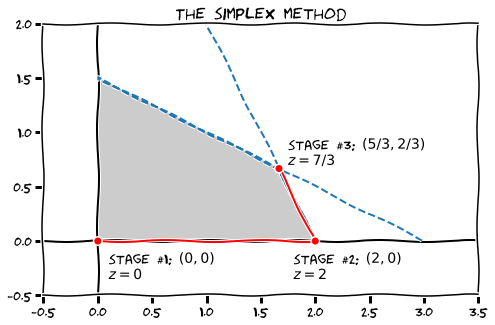
\includegraphics[width=0.75\linewidth]{images/simplex.png}
\caption{Illustration of the simplex method for Example \ref{example:FirstLinearProgram}}
\label{figure:simplexmethod}
\end{figure}
\end{example}

\begin{example}
What happens if the program does not have a unique solution?  Can the simplex method offer this information? Consider for $f(x,y)=x+\tfrac{1}{2}y$ the program
\begin{equation*}
(LP): \begin{cases} 
\displaystyle{\max_{(x,y)\in\field{R}^s} f(x,y)} \\
2x+y \leq 4 \\
x+2y \leq 3 \\
x \geq 0, y \geq 0
\end{cases}
\end{equation*}
Once in standard form, this program has the tableau
\begin{equation*}
\begin{bmatrix} 
1 & -1  & -1/2 & 0   & 0   & 0 \\
0 & 2   & 1    & 1   & 0   & 4 \\
0 & 1   & 2    & 0   & 1   & 3 \\ \hline
z & x_1 & x_2  & x_3 & x_4
\end{bmatrix}
\end{equation*}
The initial solution gives 
\begin{equation*}
z=0 \qquad \underbrace{x_3=4, \quad x_4=3}_{\text{basic solutions}} \qquad \underbrace{x_1=x_2=0}_{\text{non-basic solutions}}
\end{equation*}
There is an entering variable at $x_1$, that has to be pivoted with the second row:
\begin{equation*}
\begin{bmatrix} 
1 & -1  & -1/2 & 0   & 0   & 0 \\
0 & 1   & 1/2  & 1/2 & 0   & 2 \\
0 & 1   & 2    & 0   & 1   & 3 \\ \hline
z & x_1 & x_2  & x_3 & x_4
\end{bmatrix} \to 
\begin{bmatrix} 
1 & 0   & 0    & 1/2  & 0   & 2 \\
0 & 1   & 1/2  & 1/2  & 0   & 2 \\
0 & 0   & 3/2  & -1/2 & 1   & 1 \\ \hline
z & x_1 & x_2  & x_3  & x_4
\end{bmatrix}
\end{equation*}
The solution at this stage---which already offers an optimal solution of the program $(LP)$---gives
\begin{equation*}
z=2 \qquad \underbrace{x_1=2, \quad x_4=1}_{\text{basic solutions}} \qquad \underbrace{x_2=x_3=0}_{\text{non-basic solutions}}
\end{equation*}
Notice now that at this point we could increase the value of the coefficient of the variable $x_2$ without changing the value of $z$.
\begin{equation*}
\begin{bmatrix} 
1 & 0   & 0    & 1/2  & 0   & 2 \\
0 & 1   & 1/2  & 1/2  & 0   & 2 \\
0 & 0   & 1    & -1/3 & 2/3 & 2/3 \\ \hline
z & x_1 & x_2  & x_3  & x_4
\end{bmatrix} \to 
\begin{bmatrix} 
1 & 0   & 0    & 1/2  & 0    & 2 \\
0 & 1   & 0    & 2/3  & -1/3 & 5/3 \\
0 & 0   & 1    & -1/3 & 2/3  & 2/3 \\ \hline
z & x_1 & x_2  & x_3  & x_4
\end{bmatrix}
\end{equation*}
The solution at this stage gives
\begin{equation*}
z=2 \qquad \underbrace{x_1=5/3, \quad x_2=2/3}_{\text{basic solutions}} \qquad \underbrace{x_3=x_4=0}_{\text{non-basic solutions}}
\end{equation*}
We have found two different optimal solutions of the program $(LP)$ using the simplex method: $(2,0)$ and $(5/3, 2/3)$.  Notice that in this case, any other point in the segment joining those two points, must also be a solution.  Namely: for any $t \in [0,1]$, the point $\big(2-\tfrac{1}{3}t, \tfrac{2}{3}t \big)$ satisfies
\begin{align*}
&f\big(2-\tfrac{1}{3}t, \tfrac{2}{3}t \big) = 2 - \tfrac{1}{3}t + 2\tfrac{1}{3}t = 2. &&\text{(The value is always 4)} \\
&2\big( 2-\tfrac{1}{3}t \big) + \tfrac{2}{3}t = 4 &&(\text{The first constraint is satisfied}) \\
&2-\tfrac{1}{3}t + 2 \tfrac{2}{3}t = 2 + t \leq 3 &&(\text{The second constraint is satisfied}) \\
&2 - \tfrac{1}{3}t \geq \tfrac{5}{3} > 0 &&(\text{The third constraint is satisfied}) \\
&\tfrac{2}{3}t \geq 0 &&  (\text{The fourth constraint is satisfied})
\end{align*}
\end{example}


\begin{example}
What happens if we are unable to employ Rule 1 from the simplex method?  This situation arises on the program from Example \ref{example:FirstLinearProgram}:
\begin{equation*}
\begin{bmatrix}
1 & \boldsymbol{-2} & 2  & 3  & 0 & 0 & 0 & 0\\
0 & 1  & -1 & -3 & 2 & 1 & 0  & 3 \\
0 & -1 &  1 & 2  & 0 & 0 & -1 & 2 \\ \hline
z & x_1 & x_2 & x_3 & x_4 & x_5 & x_6
\end{bmatrix}
\end{equation*}
The first entering variable is $x_1$.  The only row we may use to pivot is the second:
\begin{equation*}
\begin{bmatrix}
1 & 0  & 0  & \boldsymbol{-3} & 4 & 2 & 0 & 6\\
0 & 1  & -1 & -3 & 2 & 1 & 0  & 3 \\
0 & 0  & 0  & -1 & 2 & 1 & -1 & 5 \\ \hline
z & x_1 & x_2 & x_3 & x_4 & x_5 & x_6
\end{bmatrix}
\end{equation*}
The next entering variable is $x_3$, but there are no possible rows to pivot.  The program is \emph{unbounded}\index{Program!unbounded}: if we increase the value of $x_3$, the value of $z$ increases (on the first row), and so do the values of the basic variables (on the other rows).
\end{example}

%!TEX root = main.tex

\section{The Frank-Wolfe Method}\index{Frank-Wolfe method}\index{Conditional-Gradient method|see {Frank-Wolfe method}}

Also known as the \emph{Conditional-Gradient method}, it is widely used to solve programs where the feasibility region $S$ is described by a system of linear inequalities.
\begin{equation*}
(P): \begin{cases} \displaystyle{\min_{\x\in S}f(\x)} \\ S=\{ \x \in \field{R}^d:  \langle \boldsymbol{a}_k, \x \rangle \leq b_k \text{ with } \boldsymbol{a}_k \in \field{R}^d, b_k \in \field{R}, 1\leq k \leq \ell  \}
\end{cases}
\end{equation*}

This is an iterative method that, at any feasible initial guess $\x_0 \in S$, considers an associated linear program $(LP_0)$ that minimizes the linear approximation $L_0(\x) = f(\x_0) + \langle \gradient{f}(\x_0), \x - \x_0 \rangle$ on the same feasible region $S$.
\begin{equation*}
(LP_0): \begin{cases} \displaystyle{\min_{\x \in S} \langle \gradient{f}(\x_0), \x-\x_0 \rangle} \\
 S =\{ \x \in \field{R}^d:  \langle \boldsymbol{a}_k, \x \rangle \leq b_k \text{ with } \boldsymbol{a}_k \in \field{R}^d, b_k \in \field{R}, 1\leq k \leq \ell  \}
 \end{cases}
\end{equation*}
Once an optimal solution $\bar{\x}_0$ of $(LP_0)$ has been obtained, a line-search\index{Line-search} is performed on the segment joining $\x_0$ with $\bar{\x}_0$ (which by hypothesis is contained in the feasibility region $S$). 
\begin{equation*}
t_0 = \argmin_{0\leq t \leq 1} f\big(\x_0 + t(\bar{\x}_0-\x_0) \big).
\end{equation*}
Set then $x_1 = \x_0 + t_0 (\bar{\x}_0-\x_0)$.  We repeat this process to obtain a sequence $\{\x_n\}_{n\in\field{N}}$ of feasible points.

We usually devise a \emph{stopping criteria} (given a fixed tolerance $\varepsilon>0$) to guarantee that we are close enough to the optimal solution of $(P)$.  An example of such a process is illustrated below:\index{Frank-Wolfe method!stopping criteria}\index{Frank-Wolfe method!lower bound}\index{Frank-Wolfe method!upper bound}
\begin{description}
\item [Initialization] Let $\x_0 \in S$ be an initial feasible guess, and set $LB=-\infty$, $UB=f(\x_0)$---the \emph{lower} and \emph{upper} bounds (respectively) for the stopping criteria.
\item [Iteration] Assume we have $\x_n$, $LB$, $UB$.  Set 
\begin{equation*}
L_n(\x) = f(\x_n) + \langle \gradient{f}(\x_n), \x-\x_n \rangle. 
\end{equation*}
Find
\begin{align*}
\bar{\x}_n &= \argmin_{\x \in S} L_n(\x) = \argmin_{\x \in S} \langle \gradient{f}(\x_n), \x-\x_n \rangle,\\
\xi_n &= \min_{\x \in S} L_n(\x) = L_n(\bar{\x}_n),\\
t_n &= \argmin_{0 \leq t \leq 1} f\big(\x_n + t(\x_n - \bar{\x}_n)\big), \\
\x_{n+1} &= \x_n + t_n (\x_n - \bar{\x}_n), \\
LB &= \max(LB, \xi_n)
\end{align*}
\item [Stopping Criteria] If $\lvert UB-LB \rvert \leq \varepsilon$, then stop. Otherwise, update the upper bound, $UB = f(\x_{n+1})$, and perform the next \textbf{Iteration}.
\end{description}

\begin{example}\label{example:FrankWolfe}
Let us use this technique to try and find the minimum value of the function $f(x,y)=(x-3)^2+(y-2)^2$ over the square with vertices at $(-3/2, 0)$, $(0, 3/2)$, $(3/2, 0)$ and $(0, -3/2)$. We start by defining the inequality constraints:
\begin{align*}
g_1(x,y) &= x+y-\tfrac{3}{2} = \langle [1,1], [x,y] \rangle - \tfrac{3}{2} \\
g_2(x,y) &= x-y-\tfrac{3}{2} = \langle [1,-1], [x,y] \rangle - \tfrac{3}{2} \\
g_3(x,y) &= -x-y-\tfrac{3}{2} = \langle [-1,-1], [x,y] \rangle - \tfrac{3}{2} \\
g_4(x,y) &= -x+y-\tfrac{3}{2} = \langle [-1,1], [x,y] \rangle - \tfrac{3}{2}
\end{align*}
\begin{figure}[ht!]
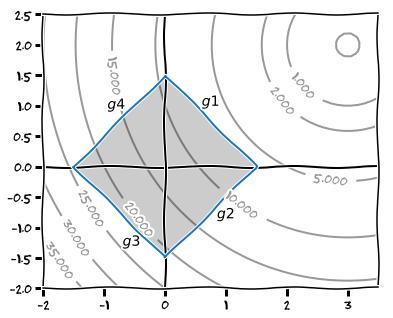
\includegraphics[width=0.75\linewidth]{images/frankwolfesetup.png}
\caption{Set up for example \ref{example:FrankWolfe}}\label{figure:FrankWolfesetup}
\end{figure}
We also need the gradient of $f$: $\gradient{f}(x,y) = \big[ 2(x-3), 2(y-2) \big]$. At any point $(x_0,y_0)$, the linear approximation needed for this method is given by
\begin{align*}
L_0(x,y) &= f(x_0,y_0) + \langle \gradient{f}(x_0, y_0), (x-x_0,y-y_0) \rangle \\
&= (x_0-3)^2 + (y_0-2)^2 + 2(x_0-3)(x-x_0) + 2(y_0-2)(y-y_0).
\end{align*}
Let's assume that the initial guess is $(0,0)$.  At this point, we set up $LB=-\infty$, and $UB=f(0,0)=13$.  According to our description of Frank-Wolfe, we have to solve at this step the program
\begin{equation*}
(LP_0): \begin{cases} \min_{(x,y) \in S} \big( -6x-4y \big) \\ S = \{ (x,y) \in \field{R}^2 : g_k(x,y) \leq 0, 1 \leq k \leq 4 \} \end{cases}
\end{equation*}
The KKT conditions request a point $(x,y) \in S$, and multipliers $\lambda_k \geq 0$ so that $\lambda_k g_k(x,y) = 0$ for $1\leq k \leq 4$, and
\begin{equation}\label{equation:secondKKTcondition}
[-6,-4] + \lambda_1 [1,1] + \lambda_2 [1,-1] + \lambda_3 [-1,-1] + \lambda_4 [-1,1] = [0,0].
\end{equation}
A quick inspection shows that there are no optimal solutions on the interior of $S$.  It must be located on one of the borders. 
\begin{description}
\item[Case 1] The four corners of $S$ are always candidates.  Notice that
\begin{align*}
f\big(\tfrac{3}{2}, 0\big) &= \tfrac{9}{4}, & f\big(-\tfrac{3}{2}, 0\big) &= \tfrac{81}{4}, &
f\big(0, \tfrac{3}{2}\big) &= \tfrac{1}{4}, & f\big(0, -\tfrac{3}{2}\big) &= \tfrac{49}{4}. 
\end{align*}
\item[Case 2] If the point is not a corner, and belongs in the border associated to $g_1$, it must be $\lambda_2=\lambda_3=\lambda_4=0$.  In this case, the second KKT condition \eqref{equation:secondKKTcondition} will never be satisfied. 
\item[Cases 3,4,5] Similarly, we infer that there are no valid solutions in any of the single borders of $S$, except on the corners.
\end{description}
We have shown that the optimal solution of $(P'_0)$ is attained at the point $(\bar{x}_0, \bar{y}_0) = (0, 3/2)$, with $\xi_0 = -6$. We proceed to perform a line-search on the segment joining $(0,0)$ and $(0,3/2)$:
\begin{equation*}
t_0 = \argmin_{0 \leq t \leq 1} f\big(0, \tfrac{3}{2}t \big) = \argmin_{0 \leq t \leq 1} \big[ 9 + \big(\tfrac{3}{2}t-2 \big)^2 \big] = \tfrac{4}{3}.
\end{equation*}



\end{example}
%!TEX root = main.tex

\section*{Exercises}

\begin{problem}[Basic]
Solve the following linear program by the simplex method:
\begin{equation*}
(LP): \begin{cases}
\displaystyle{\max_{(x,y,z) \in \field{R}^3} \big( 4x+y-z \big)} \\
x+3z \leq 6 \\
3x+y+3z \leq 9 \\
x \geq 0, y\geq 0, z\geq 0
\end{cases}
\end{equation*}
\end{problem}

\begin{problem}[Basic]
The following tableaux were obtained in the course of solving linear programs with two non-negative variables $x_1$ and $x_2$, two inequality constraints for which slack or surplus variables $x_3$ and $x_4$ were needed.  In each case, indicate whether the corresponding linear program has a unique optimum solution, has several optimum solutions (and in that case find them all), it is unbounded, or degenerate.
\begin{enumerate}
\item $\displaystyle{%
\begin{bmatrix}
1 &   0 &   3 &   2 &   0 & 20 \\
0 &   1 &  -2 &  -1 &   0 &  4 \\
0 &   0 &  -1 &   0 &   1 &  2 \\ \hline
z & x_1 & x_2 & x_3 & x_4
\end{bmatrix}
}$\smallskip
\item $\displaystyle{%
\begin{bmatrix}
1 &   0 &  -1 &   0 &   2 & 20 \\
0 &   0 &   0 &   1 &  -2 &  5 \\
0 &   1 &  -2 &   0 &   3 &  6 \\ \hline
z & x_1 & x_2 & x_3 & x_4
\end{bmatrix}
}$\smallskip
\item $\displaystyle{%
\begin{bmatrix}
1 &   2 &   0 &   0 &   1 &  8 \\
0 &   3 &   1 &   0 &  -2 &  4 \\
0 &  -2 &   0 &   1 &   1 &  0 \\ \hline
z & x_1 & x_2 & x_3 & x_4
\end{bmatrix}
}$\smallskip
\item $\displaystyle{%
\begin{bmatrix}
1 &   0 &   0 &   2 &   0 &  5 \\
0 &   0 &  -1 &   1 &   1 &  4 \\
0 &   1 &   1 &  -1 &   0 &  4 \\ \hline
z & x_1 & x_2 & x_3 & x_4
\end{bmatrix}
}$
\end{enumerate}
\end{problem}

\begin{problem}[Intermediate]
Consider the following linear program
\begin{equation*}
(LP): \begin{cases}
\displaystyle{\max_{(x,y,z) \in \field{R}^3} \big( 5x+3y+z \big)} \\
x+y+z \leq 6 \\
5x+3y+6z \leq 15 \\
x \geq 0, y \geq 0, z \geq 0
\end{cases}
\end{equation*}
Assume the following is an associated tableau:
\begin{equation*}
\begin{bmatrix}
1 &   0 &   0 &    5 &   0 &   1  & 15 \\
0 &   0 & 0.4 & -0.2 &   1 & -0.2 &  3 \\
0 &   1 & 0.6 &  1.2 &   0 &  0.2 &  3 \\ \hline
z & x_1 & x_2 &  x_3 & x_4 &  x_5  
\end{bmatrix}
\end{equation*}
\begin{enumerate}
\item What basic solution does this tableau represent? Is this solution optimal? Explain why or why not.
\item Does this tableau represent a unique optimal solution? If not, find at least three alternative optimal solutions.
\end{enumerate}
\end{problem}

% backmatter
\printindex
%!TEX root = main.tex

\bibliography{bib}
\bibliographystyle{plain}

% \nocite{peressini1988mathematics}
\nocite{finney2001thomas}
% \nocite{bertsekas1999nonlinear}
% \nocite{gautschi2011numerical}
\nocite{rudin1964principles}
\nocite{blanco2015mastering}
% \nocite{Freund2004nonlinear}
\nocite{Hunter:2007}
\nocite{dantzig1963linear}

\appendix
%!TEX root = notes.tex

\chapter{Rates of Convergence}\label{appendix:convergence}

\begin{definition}
Consider a convergent sequence $\{ \x_n \}_{n\in\field{N}} \subset \field{R}^d$ with $\xstar=\lim_n \x_n$.  We say that this sequence exhibits
\begin{description}
	\item [Linear Convergence] If there exists $0<\delta<1$ so that 
	\begin{equation*}
	\lim_n \frac{\norm{\x_{n+1} - \xstar}}{\norm{\x_n - \xstar}}=\delta.
	\end{equation*}
	We refer to $\delta$ as the \emph{rate of convergence}.
	\item [Superlinear Convergence] If 
	\begin{equation*}
	\lim_n \frac{\norm{\x_{n+1} - \xstar}}{\norm{\x_n - \xstar}}=0.
	\end{equation*}
	\item [Sublinear Convergence] If
	\begin{equation*}
	\lim_n \frac{\norm{\x_{n+1} - \xstar}}{\norm{\x_n - \xstar}}=1.
	\end{equation*}
	If, additionally, 
	\begin{equation*}
	\lim_n \frac{\norm{\x_{n+2} - \x_{n+1}}}{\norm{\x_{n+1} - \x_n}}=1,
	\end{equation*}
	we say the the sequence exhibits \emph{logarithmic convergence} to $\xstar$.
	\item [Convergence of order $q>1$] If $\x_n$ is exhibits superlinear convergence, and there exists $q>1$, $0<\delta<1$ so that 
	\begin{equation*}
	\lim_n \frac{\norm{\x_{n+1} - \xstar}}{\norm{\x_n - \xstar}^q}=\delta.
	\end{equation*}
	In particular, 
	\begin{itemize}
		\item Convergence with $q=2$ is said to be \emph{quadratic}.
		\item Convergence with $q=2$ is said to be \emph{cubic}.
		\item etc.
	\end{itemize}
\end{description}
\end{definition}

A practical method to calculate the rate of convergence of a sequence is to calculate the following sequence, which converges to $q$:
\begin{equation}\label{equation:estimateQ}
q \approx \frac{\log\big\lvert \frac{x_{n+1}-x_n}{x_n-x_{n-1}} \big\rvert}{\log\big\lvert \frac{x_n-x_{n-1}}{x_{n-1}-x_{n-2}} \big\rvert}
\end{equation}

\begin{example}
The sequence $x_n = 1/n!$ exhibits superlinear convergence, since $\lim_n \frac{1}{n!}=0$ and 
\begin{equation*}
\lim_n \frac{x_{n+1}}{x_n} = \lim_n \frac{1}{n+1} = 0.
\end{equation*}
\end{example}

\begin{example}
Given $a \in \field{R}$, $0<r<1$, the geometric sequence $\x_n = ar^n$ exhibits linear convergence, since $\lim_n ar^n = 0$ and
\begin{equation*}
\lim_n \frac{x_{n+1}}{x_n} = r < 1.
\end{equation*}
The rate of convergence is precisely $r$.
\end{example}

\begin{example}
The sequence $x_n = 2^{-2^n}$ converges to zero and is superlinear:
\begin{equation*}
\lim_n \frac{x_{n+1}}{x_n} = \lim_n 2^{-2^n} = 0
\end{equation*}
Using the estimation for $q$ given by the formula in \eqref{equation:estimateQ}, we obtain that this sequence exhibits quadratic convergence.
\end{example}

\begin{example}
The sequence $x_n = 1/n$ converges to zero and is sublinear, since
\begin{equation*}
\lim_n \frac{x_{n+1}}{x_n} = \lim_n \frac{n}{n+1} = 1.
\end{equation*}
Notice 
\begin{equation*}
\lim_n \frac{\abs{\x_{n+2} - \x_{n+1}}}{\abs{\x_{n+1} - \x_n}} = \lim_n \frac{n}{n+2} = 1;
\end{equation*}
therefore, this sequence exhibits logarithmic convergence.
\end{example}

%!TEX root = main.tex

\chapter{Basic \sympy\ commands for Calculus}\label{appendix:sympy}

A typical \sympy\ session usually starts by loading the \emph{symbols} we need, some basic functions, and basic constructors.  After that, we proceed to the description of the functions we require.

\begin{minted}[frame=single, fontsize=\footnotesize, linenos, mathescape]{python}
# Symbols, including one for infinity, $\pi$ and $e$
from sympy.abc import x,y,t,h
from sympy import oo, pi, E
# Symbols with conditions
from sympy import var
a,b = var('a,b', positive=True)

# Basic functions we may need
from sympy import sqrt, sin, cos, tan, exp, log

# Some basic symbolic manipulations may be needed
from sympy import solve, factor, expand, simplify, limit

# To do vector calculus, we need these two as well
from sympy import Matrix
from sympy.tensor.array import derive_by_array

# If in a jupyter notebook, we may want to render output as LaTeX
from sympy import init_printing
init_printing()

# Description of f
f = sin(x)/x

# A generic Rosenbrock function
# Note the symbols a, b act as parameters, while x and y act as variables
R = (a-x)**2 + b*(y-x**2)**2
\end{minted}

We are going to use these functions to perform several common operations in Calculus.

\section{Function operations}
Observe how easily we can perform all of the following:
\begin{description}
	\item[Function evaluation] with the method 
	\begin{verbatim}.subs({variable1: value1, variable2: value2, ...})\end{verbatim}
	\item[Limits] with the function \texttt{limit(object, variable, value)}.
	\item[Basic operations] with the usual operators for addition, subtraction, multiplication and division.
	\item[Composition] again with the method \texttt{.subs()}.
\end{description}

\begin{minted}[frame=single,fontsize=\footnotesize, mathescape]{python}
>>> f.subs({x: pi}) # $f(\pi)$
	0
>>> f.subs({x: 0})  # $f(0)$ --- returns "not a number"
	nan
>>> limit(f, x, 0)  # Compute $\lim_{x\to 0}f(x)$ instead
	1
>>> (f.subs({x: x+h}) - f)/h  # A divided quotient...
	(sin(h + x)/(h + x) - sin(x)/x)/h
>>> limit( (f.subs({x: x+h}) - f)/h, h, 0) # ... and its limit as $h\to 0$
	(x*cos(x) - sin(x))/x**2
\end{minted}

Notice how smart \sympy\ is in regard to the properties of symbols
\begin{minted}[frame=single,fontsize=\footnotesize, mathescape]{python}
>>> sqrt(x**2) # Square root of the square of a variable without conditions
	sqrt(x**2)
>>> sqrt(a**2) # Square root of the square of a positive variable
	a
\end{minted}

Directional limits are also possible
\begin{minted}[frame=single,fontsize=\footnotesize, mathescape]{python}
>>> limit(1/x, x, 0, dir="+")
	oo
>>> limit(1/x, x, 0, dir="-")
	-oo
\end{minted}

\section{Derivatives, Gradients, Hessians}
For functions of one variable, to obtain the symbolic derivative of a function (of any order), we usually employ the method 
\begin{verbatim} .diff(variable, order) \end{verbatim}
For functions of several variables, we employ instead 
\begin{verbatim}derive_by_array(function, list-of-variables) \end{verbatim}
If necessary, we may arrange our outputs as matrices, so we can employ proper matrix operations with them.

\begin{minted}[frame=single,fontsize=\footnotesize, mathescape]{python}
>>> f.diff(x) # $f'(x)$ without the need to mess with limits
	cos(x)/x - sin(x)/x**2
>>> f.diff(x, 2)  # $f''(x)$
	(-sin(x) - 2*cos(x)/x + 2*sin(x)/x**2)/x
>>> derive_by_array(R, [x,y]) # The gradient of R, $\gradient{R}$
	[-2*a - 4*b*x*(-x**2 + y) + 2*x, b*(-2*x**2 + 2*y)]
>>> gradient = _   # Store that in the variable 'gradient'
>>> derive_by_array(gradient, [x,y]) # The Hessian of R, $\Hess{R}$
	[[8*b*x**2 - 4*b*(-x**2 + y) + 2, -4*b*x], [-4*b*x, 2*b]]
>>> hessian = Matrix(2,2, _) # Store that as a matrix, call it 'hessian'
>>> hessian[0,0] # If we want to access the first entry of the matrix
	8*b*x**2 - 4*b*(-x**2 + y) + 2
>>> simplify(_) # Simplify that expression
	12*b*x**2 - 4*b*y + 2
>>> Delta1 = _  # Store that value as 'Delta1'
>>> hessian.det()  # Compute the determinant of the Hessian
	-16*b**2*x**2 + 2*b*(8*b*x**2 - 4*b*(-x**2 + y) + 2)
>>> Delta2 = simplify(_) # Store that value as 'Delta2'
\end{minted}

It is then a simple task (in some cases) to search for critical points by solving symbolically $\gradient{f}=0$, and checking whether they are local maxima, local minima or saddle points.
\begin{minted}[frame=single,fontsize=\footnotesize, mathescape]{python}
>>> solve(gradient, [x,y]) # Critical points of R
	[(a, a**2)]
>>> crit_points = _ # This is a list.  We call it 'crit_points' 
>>> for point in crit_points:
...     x0,y0 = point
...     print(point)
...     print("Delta1 = ", Delta1.subs({x:x0, y:y0}))
...     print("Delta2 = ", Delta2.subs({x:x0, y:y0}))
...
	(a, a**2)
	Delta1 =  8*a**2*b + 2
	Delta2 =  4*b
>>> 8*a**2*b + 2 > 0  # Is Delta1 > 0? (remember a,b>0)
	True
>>> 4*b > 0 # Is Delta2 > 0?
	True
\end{minted}
The conclusion after this small session is that any Rosenbrock function $R(x,y) = (a-x)^2 + b(y-x^2)^2$ has a global minimum at the point $(a,a^2)$.

A word of warning.  Symbolic differentiation and manipulation of expressions may not work in certain cases.  For those, numerical approximation is more suited (and incidentally, \emph{that} is the reason you are taking this course).

\begin{minted}[frame=single,fontsize=\footnotesize, mathescape]{python}
>>> solve(f.diff(x))
NotImplementedError: multiple generators [x, tan(x/2)]
No algorithms are implemented to solve equation 
x**2*(-tan(x/2)**2 + 1)/(tan(x/2)**2 + 1) - 2*x*tan(x/2)/(tan(x/2)**2 + 1)
\end{minted}

\section{Integration}

Symbolic integration for the computation of antiderivatives is also possible.  Definite integrals, while the symbolic setting allows it in many cases, it is preferably done in a numerical setting.

\begin{minted}[frame=single,fontsize=\footnotesize, mathescape]{python}
>>> R.integrate(x) # $\int R(x,y)\, dx$
	-a*x**2 + b*x**5/5 + x**3*(-2*b*y/3 + 1/3) + x*(a**2 + b*y**2)
>>> R.integrate(y) # $\int R(x,y)\, dy$
	-b*x**2*y**2 + b*y**3/3 + y*(a**2 - 2*a*x + b*x**4 + x**2)
>>> R.integrate(x, (x, 0, 1)).integrate(y, (y, 0, 1)) # $\int_0^1 \int_0^1 R(x,y)\, dx\, dy$
	a**2/4 - a/6 + 11*b/360 + 1/24
>>> f.integrate(x) # $\int \frac{\sin(x)}{x}\, dx$
	Si(x)
>>> f.integrate(x, (x, 0, pi)) # $\int_0^\pi \frac{\sin(x)}{x}\, dx$
	-2 + pi*Si(pi)
>>> _.evalf() # How much is that, actually?
	3.81803183741885
\end{minted}

\section{Sequences, series}

\begin{minted}[frame=single,fontsize=\footnotesize, mathescape]{python}
>>> 
\end{minted}

\section{Power series, series expansions}
\begin{minted}[frame=single,fontsize=\footnotesize, mathescape]{python}
>>> 
\end{minted}
%!TEX root = main.tex

\chapter{Basic graphing in Python}\label{appendix:matplotlib}

One of the advantages of doing scientific computing with Python is the wealth of different libraries we may use to represent data and functions graphically.  In this appendix we are going to do a quick overview of some of the most widely used:

\begin{enumerate}
	\item \matplotlib
	\item \texttt{bokeh}
	\item \texttt{plotly}
\end{enumerate}

\section{\matplotlib}

The \matplotlib libraries are fundamentally focused on 2D plotting.  They are open source with license based on the \emph{Python Software Foundation} (PSF) license.  If you are planning to use them for your scientific production, it is customary to cite John Hunter's 2007 seminal paper \cite{Hunter:2007}.   

In this section we are going to explore just a handful of utilities:
\begin{itemize}
 	\item The module \pyplot\, that allows us to use a similar syntax and interface as in \texttt{matlab} or \texttt{octave}
 	\item The toolkit \texttt{mplot3d} to extend \matplotlib\ for simple 3D plotting.
 	\item The toolkits \texttt{basemap} and \texttt{cartopy} to extend \matplotlib\ for projection and Geographic mapping.
 	\item The toolkit \texttt{ggplot} for those of you familiar with the \texttt{R} plotting system.
 \end{itemize} 

Let's start with a simple example or usage of the module \pyplot\.  We are going to use exclusively the Rosenbrock function $\mathcal{R}_{1,1}$.

\begin{minted}[frame=single, fontsize=\footnotesize, linenos, mathescape]{python}
import numpy as np, matplotlib.pyplot as plt 

def R(x,y): return (1.0-x)**2 + (y - x**2)**2
\end{minted}

For each plot, we usually indicate in our session the intent to create a \emph{figure}.  At that point it is customary to impose the size of the figure, number of subplots (if more than one), kind of axis, usage of grid, etc.  This is what we call the \emph{layout} of our diagrams.  For instance, to create a simple plot (with size $5 \times 10.5$) of the graph of $f(x) = \mathcal{R}(x,1)$ for $-2 \leq x \leq 2$, but focusing only in the window $[-2.5,2.5] \times [-0.5, 10]$, we issue the following commands:

\begin{minted}[frame=single,fontsize=\footnotesize, mathescape]{python}
>>> x = np.linspace(-2, 2)         # $-2 \leq x \leq 2$

>>> plt.figure(figsize=(5,10.5));  # Create a figure of requested size
... plt.axes(aspect='equal');      # I want x's and y's to be the same size
... plt.grid();                    # I want a grid
... plt.xlim(-2.5, 2.5);           # Set my window
... plt.ylim(-0.5, 10);
... plt.plot(x, R(x,1.0));         # Just plot it...
... plt.show()                     # ...and request it shows in screen
\end{minted}

See Figure \ref{figure:basicplt}, left.

It is possible to combine several plots on the same figure:

\begin{minted}[frame=single,fontsize=\footnotesize, mathescape]{python}
>>> plt.figure(figsize=(5,10.5));
... plt.axes(aspect='equal');  
... plt.grid();
... plt.xlim(-2.5, 2.5);
... plt.ylim(-0.5, 10);
... for section in range(1,6):     # Do 5 plots: R(x,n)
...     plt.plot(x,R(x,section))   # where n=1,2,3,4,5
...
... plt.show()
\end{minted}

See Figure \ref{figure:basicplt}, center.

It is hard to see which graph corresponds to which function, in spite of the different chosen colors.  We solve this issue this by allowing each graph to be labeled, and placing a legend in the diagram:

\begin{minted}[frame=single,fontsize=\footnotesize, mathescape]{python}
>>> plt.figure(figsize=(5,10.5));
... plt.axes(aspect='equal');  
... plt.grid();
... plt.xlim(-2.5, 2.5);
... plt.ylim(-0.5, 10);
... for section in range(1,6):     # The labels go here
...     plt.plot(x,R(x,section), label=section)  
...
... plt.legend()                   # The legend is requested here
... plt.show()
\end{minted}

See Figure \ref{figure:basicplt}, right.

\begin{figure}[ht!]
\begin{tabular}{ccc}
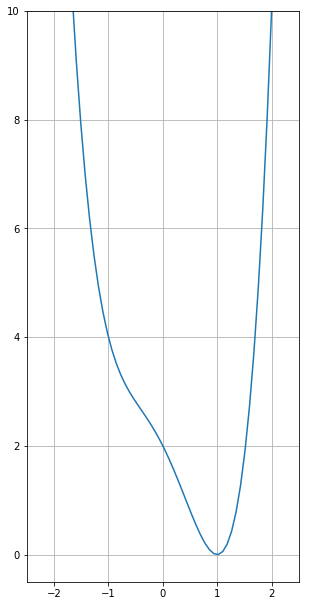
\includegraphics[width=0.33\linewidth]{images/basicplt.png} &
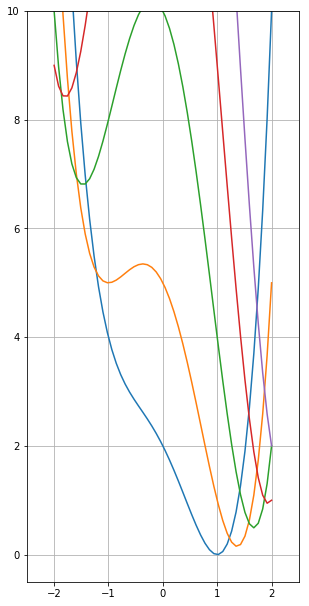
\includegraphics[width=0.33\linewidth]{images/4plotsplt.png} &
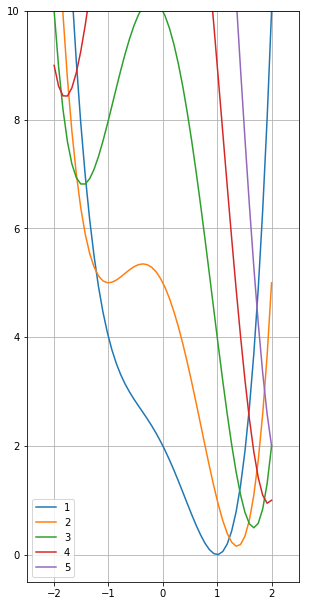
\includegraphics[width=0.33\linewidth]{images/4plotslegendplt.png}
\end{tabular}
\caption{Basic rendering of functions with \pyplot}
\label{figure:basicplt}
\end{figure}

It is possible to control more detail of your plots.  See for example how we modify line width, type, color, etc.  As an exercise, try to comment each line indicating what modifications have been performed on the corresponding graphs.

\begin{minted}[frame=single,fontsize=\footnotesize, mathescape]{python}
>>> plt.figure();                  # Let pyplot choose size and layout
... plt.plot(x, R(x,1), 'r-', lw=0.5);
... plt.plot(x, R(x,2), 'b--',lw=2);
... plt.plot(x, R(x,3), 'go');
... plt.plot(x, R(x,4), 'y-.');
... plt.show()
\end{minted}

\begin{figure}[ht!]
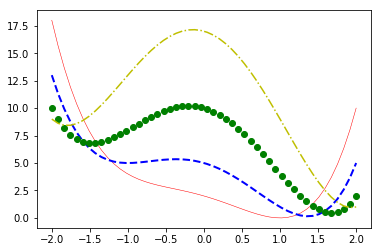
\includegraphics[width=0.75\linewidth]{images/intermediateplt.png}
\caption{Tinkering with color, style and width of lines in \pyplot}
\label{figure:intermediateplt}
\end{figure}

To plot a set of level lines (a countour plot), we can either do that manually, or request \pyplot\ to do it for us.  For instance to render the level lines $\mathcal{R}_{1,1}(x,y)=c$ for $c=1,2,3,5,10,15,20$ over the window $[-2,2] \times [-2,3]$, we could issue the following commands:

\begin{minted}[frame=single,fontsize=\footnotesize, mathescape]{python}
>>> y = np.linspace(-2,3)          # $-2 \leq y \leq 3$
>>> X,Y = np.meshgrid(x,y)         # generate the window

>>> plt.figure();                  # Let pyplot choose size and layout
... plt.contour(X, Y, R(X,Y), levels=[1,2,3,5,10,15,20]);
... plt.show()
\end{minted}

See Figure \ref{figure:contourplt}, left.

Although each level line has been rendered with a different color, it is hard to see which one is which.  Placing a legend on an already cluttered diagram may not be the best option.  Fortunately, there is a neat method to display relevant information of top of each level line:

\begin{minted}[frame=single,fontsize=\footnotesize, mathescape]{python}
>>> plt.figure();                  # Let pyplot choose size and layout
... CS = plt.contour(X, Y, R(X,Y), levels=[1,2,3,5,10,15,20]);
... plt.clabel(CS, fontsize=9, inline=1);
... plt.show()
\end{minted}

See Figure \ref{figure:contourplt}, right.

\begin{figure}[ht!]
\begin{tabular}{cc}
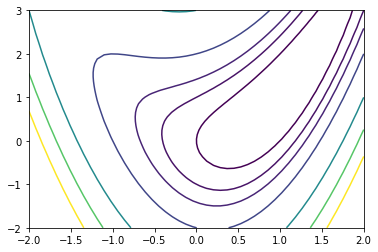
\includegraphics[width=0.5\linewidth]{images/contourplt.png} &
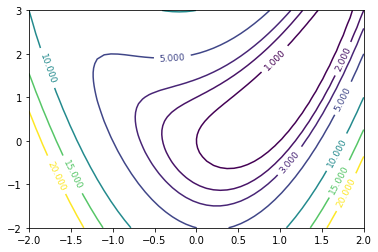
\includegraphics[width=0.5\linewidth]{images/contourplusplt.png}
\end{tabular}
\caption{Contour plots with \pyplot}
\label{figure:contourplt}
\end{figure}

\end{document}